\documentclass[letterpaper, 10 pt, conference]{ieeeconf}

\IEEEoverridecommandlockouts                              % This command is only needed if 
% you want to use the \thanks command

\overrideIEEEmargins 




\usepackage{setspace}
\usepackage{epsfig}  % for figures
\usepackage{epstopdf}
\usepackage{hyperref}

\usepackage{amssymb,amsmath, mathtools}
\usepackage{mathrsfs} 

\let\labelindent\relax
\usepackage{enumitem}
\usepackage{subfiles}

\usepackage{caption}
\usepackage{subcaption}
\captionsetup{font=footnotesize}



\makeatletter
\newcommand{\removelatexerror}{\let\@latex@error\@gobble}
\makeatother
\usepackage{xcolor}
\usepackage[ruled, vlined]{algorithm2e}
\newcommand\mycommfont[1]{\footnotesize\em\textcolor{blue}{#1}}
\SetCommentSty{mycommfont}

\SetAlFnt{\small}

\usepackage{lipsum}
\usepackage{cite}
\usepackage{thmtools,thm-restate}
\usepackage{multicol}
\usepackage{multirow}
\usepackage{bm}
%\theoremstyle{definition}
\newtheorem{definition}{Definition}[section]
\newtheorem{proposition}{Proposition}[section]
\newtheorem{lemma}{Lemma}[section]
\newtheorem{example}{Example}[section]
\newtheorem{theorem}{Theorem}[section]
\newtheorem{alg}{Algorithm}[section]
\newtheorem{corollary}{Corollary}[section]
%\theoremstyle{remark}
\newtheorem{remark}{Remark}[section]
\newtheorem{assumption}{Assumption}[section]
\newtheorem{conjecture}{Conjecture}[section]
\newtheorem{claim}{Claim}[section]
\newtheorem{property}{Property}[section]
\newtheorem{condition}{Condition}[section]
\newcommand{\vect}[1]{\boldsymbol{#1}}

\renewcommand\thetheorem{\arabic{section}.\arabic{theorem}}
\renewcommand\theproposition{\arabic{section}.\arabic{proposition}}
\renewcommand\thelemma{\arabic{section}.\arabic{lemma}}
\renewcommand\thecorollary{\arabic{section}.\arabic{corollary}}
\renewcommand\theconjecture{\arabic{section}.\arabic{conjecture}}
\renewcommand\thedefinition{\arabic{section}.\arabic{definition}}
\renewcommand\thecondition{\arabic{section}.\arabic{condition}}
\renewcommand\theassumption{\arabic{section}.\arabic{assumption}}
\renewcommand\thealg{\arabic{section}.\arabic{alg}}

\newcommand{\conv}{\textup{conv}}
\newcommand{\specificthanks}[1]{\@fnsymbol{#1}}% Inserts a specific \thanks symbol
\newcommand{\vertiii}[1]{{\left\vert\kern-0.25ex\left\vert\kern-0.25ex\left\vert #1 
    \right\vert\kern-0.25ex\right\vert\kern-0.25ex\right\vert}}

\DeclareMathOperator*{\argmin}{arg\,min}
\DeclareMathOperator*{\argmax}{arg\,max}


% SETH'S MATH
\providecommand{\sW}{\mathcal{W}}
\providecommand{\sF}{F}
\providecommand{\sP}{\mathcal{P}}
\providecommand{\sL}{\mathcal{L}}
\providecommand{\sN}{\widetilde{\mathcal{N}}}
\providecommand{\Tcs}{T^{\textup{cc}}}
\providecommand{\Tc}{\widetilde{T}^{\textup{cc}}}
\providecommand{\lyap}{\mathcal{L}}
\providecommand{\Tdl}{T^{\textup{dl}}}
\providecommand{\Tdlk}{T^{\textup{rd}}}
\newcommand{\diam}{\textup{diam}}
\newcommand{\M}{\bm{M}}
\newcommand{\A}{\bm{A}}
\newcommand{\HM}{\bm{H}}
\renewcommand{\thefootnote}{\arabic{footnote}}

%% NEW NOTATIONS!

\newcommand{\identity}{\bm{I}}
\newcommand{\barI}{\overline{I}}
%\newcommand{\barX}{\overline{x}}
\newcommand{\barX}{\overline{\bm{x}}}
\newcommand{\barG}{\overline{\mathcal{G}}}
\newcommand{\barV}{\overline{\mathcal{V}}}
\newcommand{\barE}{\overline{\mathcal{E}}}
\newcommand{\barN}{\overline{\mathcal{N}}_i}
\newcommand{\barn}{\overline{n}}
\newcommand{\nfmax}{\widetilde{n}_{f_i}}
\newcommand{\nfi}{{n}_{f_i}}
\newcommand{\gcup}{\widetilde{\mathcal{G}}}
\newcommand{\Ram}[1]{{\normalsize{\textbf{({\color{green}Ram:\ }#1)}}}}


\newcommand{\HJ}[1]{{\color{black}{#1}}}
%\renewcommand{\HJ}[1]{}
\newcommand{\rood}[1]{{\color{red}{[#1]}}}

\newcommand{\HJP}[1]{{\normalsize{\textbf{({\color{blue}Hyongju:\ }#1)}}}}

%\renewcommand{\Ram}[1]{} %uncomment this line to remove all \Ram{} tags.

% correct bad hyphenation here
\hyphenation{op-tical net-works semi-conduc-tor}


\begin{document}
	
	

%
% paper title
% Titles are generally capitalized except for words such as a, an, and, as,
% at, but, by, for, in, nor, of, on, or, the, to and up, which are usually
% not capitalized unless they are the first or last word of the title.
% Linebreaks \\ can be used within to get better formatting as desired.
% Do not put math or special symbols in the title.
\title{\LARGE \bf
	 Robust Environmental Mapping by Mobile Sensor Networks
}
%
%
% author names and IEEE memberships
% note positions of commas and nonbreaking spaces ( ~ ) LaTeX will not break
% a structure at a ~ so this keeps an author's name from being broken across
% two lines.
% use \thanks{} to gain access to the first footnote area
% a separate \thanks must be used for each paragraph as LaTeX2e's \thanks
% was not built to handle multiple paragraphs
%

\author{Hyongju~Park${}^1$, Jinsun~Liu${}^2$, Matthew~Johnson-Roberson${}^3$ and Ram~Vasudevan${}^1$
\thanks{${}^1$Hyongju Park and Ram Vasudevan are with the Department
	of Mechanical Engineering, University of Michigan, Ann Arbor,
	MI, 48109 USA {\tt\small hjcpark,ramv@umich.edu}.}% <-this % stops a space
\thanks{${}^2$Jinsun Liu is with the Robotics Institute, University of Michigan, Ann Arbor,
	MI, 48109 USA {\tt\small jinsunl@umich.edu}.}% <-this % stops a space
\thanks{${}^3$Matthew Johnson-Roberson is with the Department of Naval Architecture and Marine Engineering, University of Michigan, Ann Arbor,
	MI, 48109 USA {\tt\small mattjr@umich.edu}.}% <-this % stops a space        
}% <-this % stops a space



%\thanks{Hyongju Park is with the Department
%		of Mechanical Science and Engineering, University of Illinois at Urbana-Champaign, Urbana,
%		IL, 61801 USA {\tt\small park334@illinois.edu}.}% <-this % stops a space

%\thanks{Seth A. Hutchinson is with the Department
%of Electrical and Computer Engineering, University of Illinois at Urbana-Champaign, Urbana,
%IL, 61801 USA {\tt\small seth@illinois.edu}.}% <-this % stops a space
%\thanks{Manuscript received August 19, 2015; revised September 17, 2015.}}

% note the % following the last \IEEEmembership and also \thanks - 
% these prevent an unwanted space from occurring between the last author name
% and the end of the author line. i.e., if you had this:
% 
% \author{....lastname \thanks{...} \thanks{...} }
%                     ^------------^------------^----Do not want these spaces!
%
% a space would be appended to the last name and could cause every name on that
% line to be shifted left slightly. This is one of those "LaTeX things". For
% instance, "\textbf{A} \textbf{D}" will typeset as "A B" not "AB". To get
% "AB" then you have to do: "\textbf{A}\textbf{D}"
% \thanks is no different in this regard, so shield the last } of each \thanks
% that ends a line with a % and do not let a space in before the next \thanks.
% Spaces after \IEEEmembership other than the last one are OK (and needed) as
% you are supposed to have spaces between the names. For what it is worth,
% this is a minor point as most people would not even notice if the said evil
% space somehow managed to creep in.



% The paper headers
%\markboth{Journal of \LaTeX\ Class Files,~Vol.~13, No.~9, September~2015}%
%{Shell \MakeLowercase{\textit{et al.}}: Bare Demo of IEEEtran.cls for Journals}
% The only time the second header will appear is for the odd numbered pages
% after the title page when using the twoside option.
% 
% *** Note that you probably will NOT want to include the author's ***
% *** name in the headers of peer review papers.                   ***
% You can use \ifCLASSOPTIONpeerreview for conditional compilation here if
% you desire.




% If you want to put a publisher's ID mark on the page you can do it like
% this:
%\IEEEpubid{0000--0000/00\$00.00~\copyright~2014 IEEE}
% Remember, if you use this you must call \IEEEpubidadjcol in the second
% column for its text to clear the IEEEpubid mark.



% use for special paper notices
%\IEEEspecialpapernotice{(Invited Paper)}




% make the title area
\maketitle

% As a general rule, do not put math, special symbols or citations
% in the abstract or keywords.
\begin{abstract}
%%The Fukushima Daiichi Nuclear Power Plant (NPP) incident resulted in a heavy radiation which has hampered recovery operations for years. 
%%Real-time mapping of the spatial distribution of radioactivity near and around reactors will assist safe and cost effective restoration and prevent further contamination, which aligns with the IAEA's continuous technical support on radiation monitoring. 
%%\Ram{need just one sentence that describes what environmental mapping is and why its important.}
%%\HJ{Environment mapping is a task to build a map of spatially distributed quantity over a 2D or 3D environment, which establishes trends in environmental parameters, which can be used to prevent risks of harmful outcomes (e.g., hazardous chemical leakage, forest fire spreading, radiation contamination, flash-flooding, etc).}
%Constructing a spatially distributed map of environmental parameters such as hazardous chemical leakage, forest fires, or rain is a critical first step to effectively deploying intervention.
%Though such environmental mapping tasks could potentially be done efficiently via dispatching a group of autonomous agents, it is typically undertaken by humans due to the lack of formal methods that are able to guarantee satisfactory convergence to the true distribution.
%This paper presents a Bayesian approach to estimating spatially distributed target maps by deploying a group of mobile robots.
%The topological (locations) and spatial properties (e.g., radiation level, magnetic field strength, temperature levels, etc), which constitute the target state are unknown and are characterized by prior probability distribution over bounded domain.
%%This paper considers a continuous target domain, and robots that are equipped with noisy range sensors whose ability to detect the target varies probabilistically as a function of the distance between the robot and target.
%This paper proposes a deterministic motion model wherein robots move to maximize the observation likelihood based on their noisy sensor measurements and prior beliefs on target state. 
%In addition, a decentralized counterpart, suitable for short range sensors, is presented wherein the workspace is partitioned into multiple disjoint regions, and each robot detects target only in its associated region.
%%Belief on target state is evolved by a variant of a classical Recursive Bayesian Filter. 
%%Computing the belief propagation is generally intractable for an arbitrary target distribution due to its non-modal characteristics. 
%%An approximation scheme are developed that exploits a standardized particle filtering method.
%A suite of simulation results is presented to demonstrate the effectiveness of the proposed methods.
Constructing a spatial map of environmental parameters is crucial step to prevent hazardous chemical leakage, forest fires, or to estimate the spatially distributed physical quantities, e.g., terrain elevation/radiation. Although previous methods can do such mapping tasks efficiently via dispatching a group of autonomous agents, the satisfactory convergence to the true distribution is guaranteed only when none of the robots/sensors/agents fail. A broad class of hardware and software failures are, however, commonly found in real-world applications, and will not only undermine overall mapping performance but could be critical to human safety as well.
This paper presents a Bayesian approach for estimating an environmental parameters by deploying a group of mobile robots capable of ad-hoc communication equipped with short-range sensors. The topological (locations) and spatial properties (e.g., radiation level, magnetic field strength, temperature levels, etc), which constitute the target state are unknown and are characterized by a prior probability distribution over bounded domain. To this end, we present a general framework for coordinated multi-agent deployment aimed for good/better mapping performance even when some part of the sensors fail. First, for efficient robot-target assignment, we utilize the higher order Voronoi diagram where workspace is partitioned into disjoint regions and each region is associated with least one robots. Then, robots will be deployed to maximize the likelihood that at least one robot detects every target in their associated region. 
A suite of simulation results is presented to demonstrate the effectiveness and robustness of the proposed method compared to existing methods.

\end{abstract}

% Note that keywords are not normally used for peerreview papers.
%\begin{IEEEkeywords}
%multi-robot system, fault-tolerant algorithm, order$-k$ Voronoi diagram, coverage control, deployment.
%\end{IEEEkeywords}
%




% For peer review papers, you can put extra information on the cover
% page as needed:
% \ifCLASSOPTIONpeerreview
% \begin{center} \bfseries EDICS Category: 3-BBND \end{center}
% \fi
%
% For peerreview papers, this IEEEtran command inserts a page break and
% creates the second title. It will be ignored for other modes.
\IEEEpeerreviewmaketitle


\section{Introduction}
\label{sec:sec1}
%What is the problem?
%Why is it interesting and important?
%Why is it hard? (E.g., why do naive approaches fail?)
%Why hasn't it been solved before? (Or, what's wrong with previous proposed solutions? How does mine differ?)
%What are the key components of my approach and results? Also include any specific limitations.



%\subsection{Objective of this paper}
A team of mobile robots equipped with ad-hoc communication and sensing devices, a \emph{Mobile Sensor Network} (MSN), has a wide range of potential applications, including, exploration, surveillance, search and rescue missions, environmental monitoring for pollution detection and estimation, target tracking, cooperative detection of hazardous materials in contaminated environments, forest fire monitoring, oceanographic modeling, etc. \cite{dhillon2003sensor,cortes_coverage_2004,yu2005real} to name a few.
This paper studies environmental mapping via MSNs where an autonomous fleet with limited sensing/processing capability, trying to estimate some unknown, spatially distributed target of interest given some \textit{a priori} measurement. A few real-world application includes, building precipitation map, DEM, radiation map, heat distribution map, etc, via autonomous UAVs. 
Due to the advantages of utilizing large number of MSNs which is known to be relatively cheaper than other robots, there are considerable efforts to achieve environmental mapping via MSNs, e.g., \cite{connor2016airborne,schwager2017multi,cortez2011information,julian2012distributed,lynch2008decentralized}. To best of our knowledge, there is little to no known method that is scalable to large number of sensors, that is capable of obtaining accurate representation map of a complex environment, e.g., terrain elevation, efficiently and rapidly, and that can provide robustness to sensor failures, e.g., erroneous sensor readings, as well.
%SCALABLE TO LARGE NUMBER OF ROBOTS; AND able to SHOWN TO PROVIDE GOOD MAPPING PERFORMANCE guarantees under \rood{sensor failure, e.g., erroneous sensor readings.}
%In the past decade, estimating the unknown, spatially distributed target of interest (e.g., gas, odor, temperature, radiation, fume, etc) has received much attention from not only environmental scientists \cite{chuvieco1996mapping} but also from roboticists \cite{cortez2008smart,choi2010continuous,ristic2010information}. 
%This finds numerous applications, including environmental monitoring, pollution detection, data collection tasks, etc.
%MSNs have been shown to be ideal for such missions in that each sensors can move together and take measurements in-between or along their motions.
This paper aims to develop a class of cooperative detection model and deployment strategy, that enable for MSNs to autonomously and collectively obtain an accurate representation of an arbitrary environmental map efficiently, which has guaranteed robustness to a bounded number of sensors' failures, under the Bayesian framework.




%\subsection{Related works}
%\subsubsection{Environmental mapping using mutual information gathering}
%[ISSUE \#1: COMPUTATIONAL COMPLEXITY, SCALABILITY TO MSNs ON ENVIRONMENTAL MAPPING TASKS]
%Others have employed a non-Bayesian method to perform target distribution mapping using a single mobile robot

One of the most popular method of addressing the problem of Environmental mapping via deploying MSNs has been defining a mutual information function, and robots are controlled to follow the information gradient.
\cite{cortez2011information} has studied the multi-agent environment mapping problem, where  a mutual information gathering---utilize this idea of maximizing information gain---was used to control multiple robots to build a intensity map in a hazardous environment. Recently, \cite{schwager2017multi} has proposed algorithm utilize the gradient of mutual information to enable MSNs to estimate a map of finite events in the environment while avoiding failures due to unknown hazards. They considered probabilistic robot failure model where probability of failure of each robot depends on the distances between hazard and the robot. They utilized the history of robot failures to avoid hazardous areas. In \cite{pahlajani2014networked}, the authors considered the problem of detecting a time-inhomogeneous Poisson process concealed in the background radiation using MSNs. As was noted previously \cite{schwager2017multi, julian2012distributed}, the computational complexity for computing the \emph{information gradient}, which is used as the key control policy is exponential of the number of robots, sensor measurements and environment discretization cells. 
However, in general the computation of the gradient requires that every robot be omniscient, i.e., to have current knowledge of every other robot’s position and sensor measurements, For the reason, in most cases, mutual information-based methods are limited to small groups of robots with fully connected network. 

Also, there are studies which applied various relaxations techniques for the information gathering by robot teams to avoid the computational complexity. In \cite{julian2012distributed} proposed a fully decentralized approach where the gradient of mutual information was used to drive a network of robots for general environmental mapping tasks. They used sampling technique to reduce the size of the belief matrix for better computational efficiency. At least from the current stand, their approach has not been shown to be able to do mapping of a general complex environment, which is of our problem of interest. Their experimental results presents the case of robot fleets are inferring finite number of cell environment. In \cite{hoffmann2010mobile}, employed particle filters for approximating mutual information which enable them to use nonlinear and non-Gaussian target state and sensor models. Their methods are shown to localize a target efficiently via MSNs which maximize their information gain at each step, to name a few.
We note that all these works still assume existence of a centralized fusion center to collect the information from multiple sensors and to make a global decision.

It is worth mentioning the work of Lynch et al. \cite{lynch2008decentralized}, who devise distributed control law for MSNs to decrease the variance of their state estimate of the environment model where they utilized Average Consensus filter to propagate information among the robots. 
Their presented approach is scalable to large number of agents, fully decentralized, and should work under switching network topology as well as long as the network is connected; however their approach mainly focuses on information diffusion technique via communication among robots, and does not utilize the spatially distributed nature of the MSNs. If configured properly\footnote{One popular example of this is the work of \cite{cortes_coverage_2004} where centroidal Voronoi configuration of MSNs are proven to  achieves optimal coverage.}, MSNs are expected to handle large region environmental mapping task efficiently while maintaining minimal overlapping sensing regions.

%\subsubsection{Approaches maximizing mutual information gain}

%The particle filtering was used in this paper not due to the complexity of our algorithm; but for propagating of belief over a continues target space.


%\textbf{ISSUE \#2: NO ROBUSTNESS GUARANTEE UNDER SENSOR FAILURE}



In this paper, we present a class of computationally efficient, scalable, decentralized deployment strategies that are robust to sensor failures. 
We employ classical higher order Voronoi tessellation \cite{shamos1975closest} to achieve spatially distributed allocation of MSNs for efficient environmental mapping task.  We formulate our cost function based on a particular tessellation, and use gradient descent of the cost as our decentralized deployment strategy for MSNs. By doing so, each robot can compute gradient using merely local informations without the necessity of communicating with central server.
Thus, in our paper, the central entity is only required to fuse and update the information gathered from MSNs, but not to generate control policies for robots, which is often the case for mutual information gathering approach \cite{schwager2017multi,julian2012distributed}. Furthermore, our paper also employed particle filter along with low discrepancy sampling method for the purpose of approximating the belief of the complex, continuously distributed target efficiently, and rapidly.

Also, we present a novel combined sensor model to assign different weights to robots given a targets by taking into account the spatial relationship between robots and the target state. We derive our detection model bases on a classical binary model \cite{viswanathan1997distributed,djuric2008target} that depends on the configuration of robots. To connect the detection model to the measurement model we rely on a nonrestrictive assumption that if a robot fails to discern target from others; it may not provide the correct sensor reading for the target. This type of assumption is not new. \cite{anguelov2004detecting} has adopted similar combined sensor model which has been experimentally verified with the  laser range finder and a panoramic camera measurement. Our proposed sensor model enable us to decouple the information state from the detection tasks, such that computing the gradient is computationally sound whose complexity has turned out to be linear with respect to the number of sensors. 

We provide robustness to our method by adopting higher order Voronoi tessellation \cite{shamos1975closest} where each region from a partition is assigned to multiple robots and such redundant assignment will provide robustness to sensor failures. To best of our knowledge, almost all studies about environmental mapping by MSNs up to date have not take into account such adversarial scenarios, nor presented performance guarantee by showing convergence to ground truth value, either by analysis or by numerical simulation in the case when some part of the sensors will fail, become malicious or compromised. One exception is \cite{schwager2017multi}, who considered probabilistic robot failure model where probability of failure of each robot depends on the distances between hazard and the robot. They utilized the history of robot failures to avoid hazardous areas. The use of mutual information gradient implies that the method could potentially be robust to sensor failures. In our paper, we consider a broader class of sensor failure scenarios than that considered in \cite{schwager2017multi}. In our study, we relaxed their assumption that robot failure should depends on the location of hazards, but it can happen due to many other reasons (e.g., malicious robots, battery depletion, etc). \cite{cortez2011information} use the ordinary Voronoi tessellation for robot-target assignment. Al though these ordinary Voronoi-based approaches are considered to be the most efficient under ideal cases, such performance is not guaranteed even in the case of single sensor failure \cite{hutchinson_robust_2012}.



%\textbf{ISSUE \#3: NO CONSIDERATION OF DETECTABILITY BASED ON SPATIAL RELATIONSHIP BETWEEN ROBOTS \& ENVIRONMENT}

%[Distributed Robotic Sensor Networks--An Information Theoretic Approach]
%
%The approach are not spatially distributed (i.e., each robot has its own region) such that as their results suggest, their deployment end up having large overlapped sensing region.
%In this paper, we present a novel combined sensor model to assign different weights to robots given a targets by taking into account the spatial information. Bases on a classical noisy sensor model that depends on the the configuration of robots. Roughly speaking, if robot is distant from a target; it is more likely that it will fail to detect the target than a robot closer to a target. Intuitively, if a robot fails to discern one target from others; it is not likely to provide the correct sensor reading for the target. This type of analysis is not new, there are flora of work binary detection [REFs]. In particular, [REFs] has adopted similar model to us and experimentally verified LIDAR sensor.
%

%\subsubsection{Other related studies: multi-robot search}
%
%In particular, during mobile robot search and exploration, the Bayesian approach has enabled the construction of tools for the localization of targets \cite{bourgault2003coordinated}, target tracking \cite{stone2013bayesian}, POMDP planning \cite{candido2010exploiting}, and source localization \cite{ristic2010information,valin2007robust} (e.g., aerosol, gas, sound, chemical plume, radiation sources). 
%In this latter instance for example,  the Bayesian approach led to the development of an autonomous search algorithm that maximized information gain to find a diffusive source\cite{ristic2010information}.








The main contributions of this paper are as follows:
We propose a scalable, spatially distributed, computationally efficient, decentralized controller for MSNs which can perform environmental mapping task rapidly without a help of central entity. 
We present a novel sensor model, to remove the computational burden of maintaining mutual information by MSNs by decoupling information gathering and detection, while maintaining a satisfactory mapping performance.
We adopted higher order Voronoi tessellation for optimal robots-target assignment, in order to provide robustness under general class of sensor failures whose number is bounded.
All of which has been extensively validated via a suite of numerical simulations. 

%
%Next, we present a class of computationally efficient decentralized deployment strategies that is scalable MSNs of large size. Recall that  other approaches which requires the computation of information gradient that is, in general, computationally prohibitive. We proposed a sensor model similar to that [REFs] from which we could decouple information gathering (sensor measurement) and detection task, and proposed a cost function to be collective target detectability by MSNs.
%In this paper, we present a novel combined sensor model to assign different weights to robots given a targets by taking into account the spatial information. Bases on a classical noisy sensor model that depends on the the configuration of robots. Roughly speaking, if robot is distant from a target; it is more likely that it will fail to detect the target than a robot closer to a target. Intuitively, if a robot fails to descern target from others; it may not provide the correct sensor reading for the target. This type of analysis is not new, there are flora of work binary detection [REFs]. 
%In particular, [REFs] has adopted similar model to us and experimentally verified LIDAR sensor.
%
%Lastly, we show that our method is robust to a general class of sensor failures.
%In our paper, we consider a broader class of sensor/robot failure scenarios than that considered in \cite{schwager2017multi}. In our study, we relaxed their assumption that robot failure events should depends only on the distribution of environmental parameters, e.g., high radiation level, but not on sensor failure that could happen for many other reasons (e.g., some of the robots may be compromised, battery depletion, to name a few...) 
%
%
%



%
%As a motivating example, consider the following scenario: a team of unmanned vehicles is deployed to monitor the radiation levels over a region of interest. 
%Each vehicle is equipped with a range-limited noisy radiation sensor, to inspect the radiation level over the region of interest. 
%The vehicles must approach the radiation sources close enough to ensure detection of the source while collectively building a radiation map over the entire region.
%To perform the required mission, the group of vehicles must solve two problems: (i) \emph{robust deployment}: the vehicles must be able to distribute themselves to maximize the likelihood that the fleet can detect the target distributed over the bounded region. Thus, the collective measurements can be effectively combined to estimate the true target distribution; and (ii) \emph{map construction}: robots must be able to effectively update their posterior map using the prior believe on the map and new observations retrieved at the current configuration. 
%  it is of the uttermost importance to ensure that robots can build the spatial distribution of the radiation levels over the region of interest. To perform this task efficiently, robots should move to locations which 
% maximize the likelihood that the collective measurements are close to the true values, as well as the likelihood that every region is being monitored by at least one robot, (ii) \emph{map rebuilding}: robots should update the posterior radiation map using the prior belief on the map, and the new observations retrieved at the current configurations. 
% \textit{Problem statement:}
%\emph{The objective of this paper is to design a robust deployment and effective environmental map building strategy for the robotic network}.
%This focuses on a group of homogeneous mobile robots equipped with range sensors tasked with building a environmental map of a bounded domain where the data and the spatial coordinates of the data are correlated (e.g., precipitation map, heat distribution, radiation map, etc).
%This paper presents a novel sensor model along with a class of robust multi-robot deployment strategies under Bayesian framework, and an approximate method via Particle Filtering for efficient environmental map reconstruction.


%\Ram{describe in a single sentence how its done in this paper}

% \textit{Related works:}
%Bayesian inference has guided the development of a variety of tools to recursively estimate the state of a dynamical system and has \rood{, as a result,} provided a powerful statistical tool to manage the  uncertainties in every measurement.
%%For the reason, the method has been used extensively in robotics \cite{thrun2005probabilistic} and computer vision \cite{ponce2011computer} in the past decades. 
%%In particular, the two variants of Bayesian Filters, the Kalman Filter and Particle Filter, find a plethora of uses during Simultaneous Localization And Mapping (SLAM) which has been an extremely popular method for single to multi-robot self-navigation.
%In particular, during mobile robot search and exploration, the Bayesian approach has enabled the construction of tools for the localization of targets \cite{bourgault2003coordinated}, target tracking \cite{stone2013bayesian}, POMDP planning \cite{candido2010exploiting}, and source localization \cite{ristic2010information,valin2007robust} (e.g., aerosol, gas, sound, chemical plume, radiation sources). 
%In this latter instance for example,  the Bayesian approach led to the development of an autonomous search algorithm that maximized information gain to find a diffusive source\cite{ristic2010information}.
%%\Ram{why is this paper in particular relevant and what is the missing gap here between what they are proposing and what you are proposing in this paper??}. 
%\cite{cortez2011information,schwager2017multi} studied the multi-agent environment mapping problem, where  a mutual information gathering---utilize this idea of maximizing information gain---was used to control multiple robots to build a intensity map in a hazardous environment. Especially. \cite{schwager2017multi} considered probabilistic robot failure model where probability of failure of each robot depends on the distances between hazard and the robot. They utilized the history of robot failures to avoid hazardous areas. In our paper, we consider a broader class of sensor/robot failure scenarios than that considered in \cite{schwager2017multi}. In our study, robot failure events do not necessarily depend on the distribution of environmental parameters, e.g., radiation level. 
%\HJ{We found that the key idea of their search algorithm to maximize over the information gain can be to adopted to solve our problem; the multi-agent environmental mapping.}
%\Ram{Does your last sentence mean, that we are using their search algorithm but extending it the multi-agent case? If so, then please say that clearly.}
%\HJP{The multi-robot search problem of finding missing objects is a very different problem from ours. Our approach merely adopted their approach in that we are also maximizing over an information gain [positive detection likelihood] to determine our deployment policy. I edited the previous sentence to make this clear.} 

%Especially,  studies the information-driven autonomous search for a diffusive source where their search algorithm maximizes the information gain (i.e., entropy reduction).

%\Ram{this next paragraph needs to more clearly explain why their method (specifically the one in \cite{lilienthal2009statistical} is deficient. At the moment it seems like a nice method to solve the problem you are proposing.}

%ADD THIS PAPER BY CORTEZ ET AL.,
%\cite{cortez2011information} AND MORE RECENT PAPERS WRITTEN AFTER 2016
%QUOTE FROM REVIEWER: ``Most importantly, it appears the paper by Cortez
%et al. (see citation [C]) shares the motivating problem of
%mapping radiation, also maximizes information gain by
%following a gradient in a distributed team of mobile
%sensors. It is unclear what the novelty of the paper
%compared to [C] is.''

%Others have employed a non-Bayesian method to perform target distribution mapping using a single mobile robot \cite{lilienthal2009statistical}.
%This approach focused on trying to detect and identify gas concentration that was continuously distributed over a space.
%In this instance, the diffusive sensor, which is typically used in environmental mapping, was only able to provide information about a relatively small area compared to their sonar or laser range scan counterparts.
%To overcome the limitation, the authors proposed a novel grid-mapped technique which used a Gaussian kernel to model the decreasing likelihood that a particular reading represents the true concentration with respect to the distance from the point of measurement. 
%Despite the promising results, their method did not scale well in larger environment since it relied upon a single-robot that was deployed using a pre-specified Mowing pattern. 
%%It is worth mentioning the work of Lynch et al. \cite{lynch2008decentralized}, who devise distributed control law for MSN to decrease the variance of their state estimate of the environment where they utilized Average Consensus filter to propagate information among the robots.
%
%%While they used a non-Bayesian method, \cite{lilienthal2009statistical} is the most related work that deals with target distribution mapping---in their work, constructing concentration map---by a mobile robot where the mission is of both detection and identification of gas continuously distributed over a space. 
%%In \cite{lilienthal2009statistical}, Lilienthal and Duckett observed that measurement from diffusive sensor provides information about a relatively smaller area compared to the measurement extracted from sonar, or laser range scans. 
%%To overcome the limitation, they proposed a novel grid-mapped technique which use Gaussian weighing kernel to model the decreasing likelihood that a particular reading represents the true concentration with respect to the distance from the point of measurement. 
%%\HJ{Despite the promising results, their method does not scale well with larger environment since  they merely considers a single-robot navigation using heuristic Mowing patterns.}
%
%Similar to \cite{cortez2011information}, this paper focuses on multi-robot probabilistic search for diffusive source using multi-robot deployment strategies \cite{cortes_coverage_2004}. 
%%Again, given a limited number of robots, our main interest is optimal deployment and simultaneous mapping of spatial distribution by concurrent measurement of the quantitative information acquired from target. 
%While those studies of deployment assume a static, known prior topological target distribution, their goal is to find deployment policies that maximize the collective quantity of interest, e.g., Quality of Service (QoS), Signal-to-Noise Ratio (SNR).
%On the other hand, this presents a general framework for incremental reconstruction of spatially distributed target information map over a bounded region using new measurements made from a MSN, where sensors are dynamically reconfigured to maximize the most recent collective belief on the target distribution. 
%
%%The areas of novelty in the paper include 
%
%% \textit{Contributions:}
%This paper's primary contributions are three fold:
%first, a probabilistic sensor model that incorporates joint target detection and spatial distribution estimation by a group of mobile sensors while capturing a key characteristic of the target detection task--the probability of seeing a target, monotonically decreases as a function of the distance between the sensor and the target, which is a typical characteristic of range sensors.
%%\Ram{I still don't understand what you mean by: atypical property of range sensors. Are you trying to say that people don't typically assume that property for range sensors but it is a property of range sensors?}. 
%%\HJP{My apologies again for not making this clear. I misunderstood the meaning of the word `atypical'. I replaced the word with different one.}
%Second, a class of deployment strategies ranging from decentralized to fully coordinated ones are proposed not only to maximize the information gain but to provides relative robustness as well, which existing methods, e.g., \cite{cortez2011information} are not capable of.
%Also, we minimize the additional sensing effort---required a the cost of robustness---by adopting a general space partitioning method from computational geometry.
%%Each control law is designed to maximize the collective worst-case observation likelihood marginalized over the previous belief of the target distribution. 
%%which is halted when robots' shared belief converges such that the belief no longer changes over time. 
%Lastly, a variation of the Sequential Importance Resampling (SIR) Particle Filter---which uses the joint observations and the updated configuration of the robots---is adopted to update the posterior belief on the target efficiently via approximation.

\textit{Organizations:}
The rest of the paper is organized as follows. 
Section \ref{sec:sec2} presents notation used in the remainder of the paper, formally defines the problem of interest, and reviews a recursive Bayesian filter tailored to the problem.
Section \ref{sec:sec3} presents our combined probabilistic sensor model. 
The deployment strategy is formally presented in Section \ref{sec:sec4}. Section \ref{sec:sec6} discusses an approximate belief update method via particle filters. The robustness of our deployment and effectiveness of the belief update approach is evaluated via numerical simulations in Sections \ref{sec:sec7}. Finally, Section \ref{sec:sec9} concludes the paper and proposes a number of future directions.

%
%In this paper, we propose a class of deployment strategies for MSNs aimed for robust environmental monitoring. 
%Instead of choosing control to be directly maximizing information gain (entropy), which has been known to be notoriously computationally demanding and has no known robustness properties to failures; we pose the a constrained optimization problem and use classical spatial tessellation to derive solution model. Due to complexity of the problem, we propose gradient descent algorithm and show that state propagated by the control will mitigate the effect of unreliable measurement to be equally used to propagate the belief, 
%Deployment through the control law is extremely useful to efficiently consider observations made at different locations using different robots.




%\section{Preliminaries}
\section{Problem description}
\label{sec:sec2}

This section presents the notation used throughout the paper, an illustrative example, and the problem of interest.
%\subsection{Our system}
\subsection{Notations and Our System Definition}
\label{sec:sec21}
Throughout the text, the italic bold font is used to describe random quantities, a subscript $t$ indicates that the value is measured at time step $t$, and $\mathbb{Z}^{+}$ denotes nonnegative integers. %We may also suppress subscript $t$ if it is clear from the context. 
Given a continuous random variable $\bm{x}$, if it is distributed according to a Probability Density Function (PDF), we denote it by $f_{\bm{x}}$.
Given a discrete random variable $\bm{y}$, if it is distributed according to a Probability Mass Function (PMF), we denote it by $p_{\bm{y}}$.
Consider a group of $m$ mobile robots deployed in a workspace, i.e., ambient space, $\mathcal{Q} \subseteq \mathbb{R}^d$ where $d = 2,3$. 
This paper assumes $d=2$ though the presented framework generalizes to $d=3$. 
Let $\mathbb{S}^{d-1} = \lbrace s\in \mathbb{R}^d\mid \left\| s \right\|=1 \rbrace$ be a unit circle/sphere, then the state of $m$ robots is the set of locations and orientations at time $t$, and it is represented as an $m$-tuple $x_t = (x_t^1,\dots,x_t^m)$, where $x_t^i \in \mathcal{Q} \times \mathbb{S}^{d-1}$. We denote by the set ${x}_{0:t}\coloneqq \lbrace {x}_0,\dots,{x}_t \rbrace$ the robot states up to time $t$. 
Given a pair of states $(x_t,x_{t+1})$, robots follow a way-point-based, continuous-time, deterministic motion model with dynamic constraints:
\begin{equation}
\dot{x}_{t+1} = \textup{f}(x(l),\,u(l)), \,\,\, l \in [l_0,\,l_f]
\label{eq:constraint}
\end{equation}
with boundary conditions $x(l_0) = x_t$ and $x(l_f) = x_{t+1}$ where $u(t)$ is a control, $t_0$ is the \emph{initial time}, and $t_f$ is the \emph{final time} which is free. 
Let $u_t^{\star}$ be the \emph{optimal control policy}\footnote{In the current context, the optimal control policy is a sequence of control inputs (in discrete time domain) or control path (in continuous time domain) governed by dynamics of the vehicle. On example of such optimal control policy can be generated by Linear-Quadratic Regulator (LQR) if the dynamics were linear.} which drives robots' state from $x_t$ to $x_{t+1}$ in minimum time under the dynamic (or kinematic) constraints. Similarly, let $u_{0:t}$ be the sequence of control policies up to time $t$.
We define a \emph{target} to be a physical object or some measurable quantity spatially distributed over a bounded domain.
Let $\bm{z}$ be the \emph{target state} which is a random vector. 
The target state consists of location, $\bm{q} \in \mathcal{Q}$, and information state (quantitative information about the target), $\bm{I} \in \mathcal{I} \subseteq \mathbb{R}$.
The Cartesian product $\mathcal{Z} = \mathcal{Q} \times \mathcal{I}$ is the \emph{target state space}.
Let $\bm{y}_{t}=(\bm{y}_{t}^{1},\dots,\bm{y}_{t}^{n})$ be binary random $n$ tuple which indicates the observation made by $m$ robots at time step $t$ where each $\bm{y}_{t}^{i} \in \lbrace 0,\,1 \rbrace$, and $n$ is the dimension of the sensor input.
Let the set $\bm{y}_{1:t}\coloneqq \lbrace \bm{y}_1,\dots,\bm{y}_t \rbrace$ denote observations made by robots up to time $t$. Let $\bm{y}_{D}$ a binary random tuple of size $m$ where each $\bm{y}_{D}^i \in \lbrace 0,\,1 \rbrace$ which denotes the detection by $i$th robot.
Finally, we let $\mathcal{F} \subseteq \lbrace 1,\dots,m \rbrace$ be the index set of robots whose sensor has failed.
%\Ram{it may make sense for the subsequent development for you to mention that $y$ is a function of $z$ and $x$.}
%Note that if target location is unknown, observations made by different sensors are conditionally independent given the target location \Ram{this is missing a citation}.
%\Ram{it may also make sense for you to consider a simple example here just to formalize the notation for the reader}

%To understand this notation, consider the following real-world example.
%Suppose that one is interested in building a real-time precipitation map of a city by utilizing a group of autonomous vehicles' windshield wiper data (which provides high spatial and temporal resolution).
%In this example, the target state is made up of a location in the city and an information state associated with the instantaneous precipitation rate.
%An observation model can capture the relationship between a measured windshield wiper rate and a precipitation rate. 
%The objective of this paper is to design a deployment strategy to maximize the likelihood of rain detections and to develop a Recursive Bayesian Filter to efficiently aggregate the collected observations to generate a precipitation map.
%A proper choice of probabilistic observation model which captures the behavior of windshield wipers reasonably well, and a deployment strategy (where to send those vehicles) which maximizes the likelihood of rain detections, can be used as a sensor model, and motion model, respectively, to design a Recursive Bayesian Filter for estimating the true precipitation map. 
%Such probabilistic method can be approximated, e.g., using Particle filter, for rapid reconstruction of the map.

%\subsection{Notations and terminologies}

%\subsection{Problem Definition}

%\Ram{Is $b_t = p(z \mid x_{0:t},y_{0:t}, b_0)$}. 
%Each belief, $b_t$, depends on initial belief, $b_0$, the robots' initial configuration $x_0$, the set of controls, $u_{0:t}$, and observations up to this point, $\bm{y}_{1:t-1}$.
%\rood{In our context, we say that sensor measurement of a target by a robot is \emph{reliable}, if the target can be detected by the robot and one of its sensors correctly reports a normal reading, and \emph{unreliable} otherwise.}

\subsection{An illustrative Example: Airborne LiDAR for DEM generation}
\label{sec:sec22}
Consider a group of autonomous aerial vehicles trying to acquire an accurate Digital Elevation Model (DEM)\footnote{A digital elevation model (DEM) is a digital model or 3D representation of a terrain's surface — commonly for a planet (including Earth), moon, or asteroid -- created from terrain elevation data [THIS HAS BEEN TAKEN FROM WIKIPEDIA. I WILL NEED TO CHANGE THIS...].} of some bounded region using airborne LIDAR measurements.
The first problem is: given a finite number of vehicles, how to deploy those vehicles such that the probability that robots will fail to targets dispersed over the region of interest stays minimum. Also, it may be possible that LIDAR measurement from some part of the fleet is corrupt or unreliable which could degrade the quality of DEM. Taking such adversarial scenarios into account, it is crucial to design a deployment strategy along given a sensor model capable of fault-detection which guarantees worst-case optimal target detection performance. 
Finally, it is also important to process the measurement to update the belief on target state over time in efficient manner such tat within a reasonable time, the autonomous fleet could obtain an accurate DEM model.


\subsection{Deployment strategy for the worst-case optimal target detection under sensor failures}
\label{sec:sec23}
%Let $\bm{y}_{D}$ a binary random tuple of size $m$ where each $\bm{y}_{D}^i \in \lbrace 0,\,1 \rbrace$ which returns the detection by $i$th robot.
For a given target located at $q \in \mathcal{Q}$, 
$
p(\bm{y}_{D}^i =0 \mid x^i,\bm{q} = q)
$
is the probability that $i$th robot detected target located at $q$, and $\bm{y}_{D}^i = 1$ otherwise.
In a similar manner, the joint event $p(\bm{y}_{D}=\bm{0} \mid x, \bm{q}=q)$ is the probability that $m$ robots failed to detect the target at $q$. 
%WRITE EQUATIONS HERE....
The optimal configuration---for the case when sensors in $\mathcal{F}$ fail to operate---must satisfy:
\begin{equation}
x^{\star} = \arg
\min_{x \in \mathcal{Q}^m} 
p(y_{D} = \bm{0} \mid x, \mathcal{F})
\label{mainprob}
\end{equation}
subject to
\begin{equation}
p(y_D = \bm{0} \mid x,\bm{q}=q,\mathcal{F}) <1\,\,\,\forall q \in \mathcal{Q}.
\label{const}
\end{equation}
In other words given the sensor failure $\mathcal{F}$, for each target, there must be at least one robot that can detect it, which is an essential constraint for the environmental mapping task\footnote{Worst-case optimal (minimax) solution to the problem could lead to too conservative in these type of applications.}.
The target distribution of $\bm{q}$ has been marginalized out. Unfortunately, obtaining the global solution of even the outer minimization problem can be proven to be NP-Hard by reduction from a simpler static locational optimization problem, namely, \emph{$m$-median problem}\footnote{$m$-median problem is one of the popular locational optimization problem where the objective is to locate $m$ facilities to minimize the distance between demands and the facilities given uniform prior. The problem is NP-Hard in general graph (not necessarily a tree).}. To overcome the computational complexity, we will consider a gradient descent (greedy) approach where control policy at each time step minimizes the missed-detection probability of targets by robots at their future locations (one-step lookahead). We will utilize the higher order Voronoi tessellation [REFs] for robot target assignment, and will show that the solution given the assignment solves \eqref{mainprob}.

%We will present a gradient decent method to derive a local solution to the problem given a constant probability of failure for all robots, i.e., $p(i \in \mathcal{F}) = p_{\mathcal{F}}^i$.
%Thus, given a target $q$ distributed over $\mathcal{Q}$, with prior  distribution $f_q$, 



\subsection{Combined sensor model}
\label{sec:sec24}
Here, we make a simple assumption that given a target, a sensor can correctly measure the target only if the sensor can detect target\footnote{Successful detection of a target means that the sensor can discern the target from others.} \emph{a priori}.
Furthermore we assume that, if a sensor can detect a target, a measurement of the target by the sensor is simply corrupted by noise (e.g., Gaussian). On the other hand, of a robot fail to detect a target, the measurement given the target may be unreliable and should not be considered as a correct measurement. In other words, only the sensor measurement provided from a positive detection is considered, but others will be abandoned. These assumptions turned out to be unrestrictive according to the work of \cite{anguelov2004detecting} in which authors has experimentally verified a similar combined sensor model 
on mobile robot using laser range finder and a panoramic camera measurement.

\subsection{Environmental mapping using recursive Bayesian filter}
\label{sec:sec25}
Based on our sensor model, and the deployment strategy, we derive Bayesian filtering equation to recursively update beliefs on a particular unknown environment. 
Let $b_t$ represent a the posterior probability distribution of the target state at time $t \in \mathbb{Z}_{\geq 0}$, the initial belief $b_0$ is assumed to be uniform density if no prior information on the target is available, and let $b^{\star}$ be the \emph{true posterior belief}\footnote{We assume for now that the true posterior target distribution can be obtained, e.g., via exhaustive search and measurements made by a MSN on the target state.} 
To this end, we quantify the difference between the true posterior belief, $b^{\star}$ and an approximation using our method via the Kullback-Leibler (K-L) divergence.
%\footnote{K-L divergence is often used to measure the difference between two probability distributions; given $f_{\bm{x}},f_{\bm{y}}$,		$D_{\text{KL}} \left( \bm{x} \middle\| \bm{y} \right) = \int_{-\infty}^{\infty} f_{\bm{x}}(x)\log\left(\frac{f_{\bm{x}}(x)}{f_{\bm{y}}(y)}\right) $.}.
We demonstrate via our numerical simulation in Section \ref{sec:sec7} that for a given $\epsilon>0$ and $\mathcal{F} \neq \emptyset$, there is reasonably small $T >0$ such that if robots use the proposed deployment strategy, $t>T$ implies $D_{\text{KL}}\left(b_{t} \middle\| b^{\star}\right) < \epsilon$.

%\Ram{How do you in practice solve this problem since we do not know $b_t^*$?}



\section{Probabilistic Range-limited Sensor Model}
\label{sec:sec3}
In this section, we present our combined sensor model. Each mobile robot is equipped with a \emph{range-limited sensor} that can measure quantitative information from afar and a \emph{radio} to communicate with other nodes to share its belief. 
%% MOTIVATION....
Each range sensor measurement is corrupted by noise, and the measurement is valid only if the target is detected.
This combined sensor model joins the generic noisy sensor model with the binary detection model \cite{viswanathan1997distributed,djuric2008target}.
% The probabilistic range sensor model is, in fact, not new. 
%Anguelov et al., \cite{anguelov2004detecting} apply the Expectation Maximization (EM) algorithm to cluster different types of objects from sequences of range data, where they adopted their such combined range sensor model. 
In fact, this combined sensor model has been experimentally validated during an object mapping and detection task using a laser scanner~\cite{anguelov2004detecting}.
%Their framework was validated experimentally on real-world datasets by showing the acquisition of accurate object maps and reliable detection.
%Although the sensor model was shown to follow the actual behavior of the laser scanner well \cite{anguelov2004detecting}, 
We postulate that this model is general enough to model other range-limited sensors as well; as long as the sensor is capable of distinguishing the target from the environment, and has uniform sensing range. 
A few example sensors satisfying these characteristics are 360-degree camera, wireless antenna, Gaussmeter, heat sensor, olfactory receptor, etc.
%to find more sensors with the characteristics, refer to \cite{akyildiz2002survey} and the reference therein).
%When detecting target, we assume that binary information (i.e., detection, no detection) is available. 
%During target detection, we assume that the sensor generates binary information corresponding to a detection.
%The binary detection model is used to capture one of the main characteristic of the atypical range sensors, that is, the chance of successful detection decreases monotonically by the distance between the sensor and the target \Ram{this sentence makes no sense}.
%The method can be also generalized if multi-level detection is possible.  
While performing the detection task, we assume each sensor returns a $1$ if a target is detected or $0$ otherwise. 
The ability to detect a target for each $i^{\textup{th}}$ robot is a binary random variable $\bm{y}_D^i$ with a distribution that depends on the relative distance between the target and robot. 
%In other words, $\bm{y}_{D}^i=1$ is the event that the target is detected by the $i^{\textup{th}}$ sensor and $\bm{y}_{D}^i=0$ is the event that the target is not detected by the $i^{\textup{th}}$ sensor. 
This binary detection model, however, does not account for false positive or negatives.
For example for a given $\mathcal{F}$, the probability of the event that all $m$ sensors with configuration $x_t$ fail to detect the target located at $q \in \mathcal{Q}$ is
\begin{align}
&p_{\bm{y}_{D,t} \mid
	{x}_{t},\bm{z},\mathcal{F}}\left(
\bm{y}_{D,t} = \bm{0} \mid {x}_{t},
\bm{z}=(q,I),\mathcal{F}\right) \nonumber \\
&= \prod_{i \notin \mathcal{F}}
p_{\bm{y}_{D,t}^i \mid
	{x}_{t},\bm{q}}\left(
\bm{y}_{D,t}^i = 0 \mid
{x}_{t},\bm{q}=q\right), \nonumber
\end{align}
where $\bm{0}$ is a $m$-tuple of zeros. For measuring a quantity of interest from a given environment, we consider a generic, noisy sensor model, where each sensor reports
binary output given a target state consists of information and location.
The likelihood function at time $t$ is:
\begin{equation}
p(\bm{y}_t = \bm{1} \mid x_t, \bm{z} = (q,I)),
\label{lhd}
\end{equation}
which is the probability that $i$th robot measured the target 
with intensity value of $I$ at location $q$, i.e., positive measurement.
A general example of the likelihood function is a Gaussian, $\omega\mathcal{N}(I,I^{\star},\sigma_I^2)$ where $I^{\star}$ the ground truth intensity value at $q$, $\sigma_I^2$ is the variance of the intensity at the target located at $q$, and $\omega$ is a normalization constant. Note that since the observations made by $m$ robots are independent,
\[
p(\bm{y}_t = \bm{1} \mid x_t, \bm{z} = (q,I)) =
\prod_{i=1}^m
p(\bm{y}_t^i = 1 \mid x_t, \bm{z} = (q,I)),
\] 
or \eqref{lhd} can be obtained via other distributed sensor fusion techniques (see e.g., \cite{stroupe2001distributed}).
In our sensor model, we assume that the random vector $\bm{y}$ depends on $\bm{y}_D$ which is a random $m$-tuple corresponds to detection by $m$ robots such that $\bm{y}_D = (\bm{y}_D^1,\dots,\bm{y}_D^m)$ where $\bm{y}_D^i \in \lbrace 0,\,1 \rbrace$ for all $i$ when conditioned on $x_t,\bm{z}$, so that the conditional PDF can be computed as:
\begin{align*}
&f_{\bm{y}_t \mid \bm{z},x_{t},\mathcal{F}}(\bm{y_t}=\bm{1} \mid z,x_{t},\mathcal{F}) \\
&=f_{\bm{y}_t \mid \bm{z},x_{t},\bm{y}_{D,t},\mathcal{F}}(\bm{y_t}=\bm{1} \mid z,x_{t},\bm{y}_{D,t} \neq \mathbf{0},\mathcal{F}) \\ 
&\,\,\,\,\,\,\,\times p_{\bm{y}_{D,t} \mid \bm{z},x_{t},\mathcal{F}}(\bm{y}_{D,t} \neq \mathbf{0} \mid z,x_{t},\mathcal{F}) \nonumber\\
&+f_{\bm{y}_t \mid \bm{z},x_{t},\bm{y}_{D,t},\mathcal{F}}(\bm{y_t}=\bm{1} \mid z,x_{t},\bm{y}_{D,t}=\mathbf{0},\mathcal{F}) \\
&\,\,\,\,\,\,\,\times p_{\bm{y}_{D,t} \mid \bm{z},x_{t},\mathcal{F}}(\bm{y}_{D,t} =\mathbf{0} \mid z,x_{t},\mathcal{F}), \nonumber
\end{align*}
where $\bm{y}_D \neq \mathbf{0}$ means there is $j \in \lbrace 1,\dots,m \rbrace$ such that $\bm{y}_D^j = 1$ and $\bm{y}_D = \mathbf{0}$ means $\bm{y}_D^j = 0$ for all $j \in \lbrace 1,\dots,m \rbrace$. 
If target is missed-detected, i.e., $\bm{y}_{D,t} =\bm{0}$, the measurement is random which is modeled by uniform density, i.e.,
\begin{align*}
&f_{\bm{y}_t \mid \bm{z},x_{t},\bm{y}_{D,t},\mathcal{F}}(\bm{y}_t = \bm{1} \mid z,x_{t},\bm{y}_{D,t}=\mathbf{0},\mathcal{F}) \\
&=f_{\bm{y}_t \mid \bm{z},x_{t},\bm{y}_{D,t}}(\bm{y}_t = \bm{1} \mid z,x_{t},\bm{y}_{D,t}=\mathbf{0})= I_{\textup{range}}^{-1}
\end{align*}
where $I_{\textup{range}} := I_{\max} - I_{\min}$. By the law of total probability, we have
%\begin{align*}
%&p_{\bm{y}_{D,t} \mid \bm{z},x_{t-1},u_t,\mathcal{F}}(\bm{y}_{D,t} =\mathbf{0}  \mid z,x_{t-1},u_t,\mathcal{F}) \\
%&= 1-p_{\bm{y}_{D,t} \mid \bm{z},x_{t-1},u_t,\mathcal{F}}(\bm{y}_{D,t} \neq \mathbf{0} \mid z,x_{t-1},u_t,\mathcal{F}).
%\end{align*}
\begin{align}
&f_{\bm{y}_t \mid \bm{z},x_{t},\mathcal{F}}(\bm{y}_t = \bm{1} \mid z,x_{t},\mathcal{F}) \nonumber \\
&=(1-
\underbrace{
p_{\bm{y}_{D,t} \mid \bm{z},x_{t},\mathcal{F}}(\bm{y}_{D,t} = \mathbf{0} \mid z,x_{t},\mathcal{F}))}_{\textup{ }(\star) \textup{ the probability of missded detection}} \nonumber 
\end{align}
\begin{align}
&\,\,\,\,\,\,\,\times \underbrace{f_{\bm{y}_t \mid \bm{z},x_{t}\bm{y}_{D,t},\mathcal{F}}(y_t \mid z,x_{t},\bm{y}_{D,t}\neq \mathbf{0},\mathcal{F})}_{\textup{the likelihood of reliable measurements}}, \nonumber \\
&+I_{\textup{range}}^{-1}p_{\bm{y}_{D,t} \mid \bm{z},x_{t},\mathcal{F}}(\bm{y}_{D,t} = \mathbf{0} \mid z,x_{t},\mathcal{F})
\label{eq10}
\end{align}
By minimizing $(\star)$, one can ensure that only reliable measurements on the target state is considered. 

%We are merely interested in maximizing \rood{marginal} likelihood of reliable measurements \rood{where the target state $z$ has been marginalized out}.

%the first term become dominant when it is more likely that all robots fails to detect a target, and in that case, a randomized measurement will be considered. On the other hand, the second term become dominant when it is more likely that robots are able to detect the target and in that case the measurement will be merely corrupted by noise. Note that $m$ observation distributions can be merged to compute the term, $f_{\bm{y}_t \mid \bm{z},x_{t-1},u_t,\bm{y}_{D,t}}(y_t \mid z,x_{t-1},u_t,\bm{y}_{D,t} \neq \mathbf{0})$ via distributed sensor fusion techniques (see e.g., \cite{stroupe2001distributed}).
%
%Thus, for a given target located at $q \in \mathcal{Q}$,
%\begin{align*}
%&b_t(I\mid\bm{q}=q) \\
%&= \eta_t f_{\bm{y}_t\mid x_t,\bm{z}} \left(
%y_t^i \mid x_t,z \right) b_{t-1}(I \mid \bm{q}=q)\\
%&=\eta_t p_{\bm{y}_D \mid \bm{z},x}(\bm{y}_D = \mathbf{0} \mid z,x)  
%( I_{\textup{range}}^{-1} \\
%&- f_{\bm{y} \mid \bm{z},x,\bm{y}_D^i}(y^i \mid z,x,\bm{y}_D\neq \mathbf{0})) b_{t-1}(I \mid \bm{q}=q)\\
%&+ f_{\bm{y} \mid \bm{z},x,\bm{y}_D^i}(y \mid z,x,\bm{y}_D\neq \mathbf{0})b_{t-1}(I \mid \bm{q}=q).
%\end{align*}
%
%
%

%
%\noindent(WILL BE REMOVED...)
%\begin{equation}
%f_{\bm{y}^i \mid \bm{z},x}(y^i \mid z,x) = p_{\bm{y}_D^i \mid \bm{z},x}(\bm{y}_D^i=y_D^i \mid z,x)f_{\bm{y}_I^i \mid \bm{z},x}(y_I^i \mid z,x)
%\nonumber
%\end{equation}
%where $y_D^i \in \lbrace 0,1 \rbrace$ for all $i \in \lbrace 1,\dots,n \rbrace$.
%Since the set of observations $\bm{y}^1,\dots,\bm{y}^m$ are made independently by $m$ sensors, the joint probability distribution by $m$ sensors, given a target at $z$ becomes:
%
%\begin{align}
%&f_{\bm{y}_t\mid x_t,\bm{z}}
%\left(
%y_t
%\mid x_t,z
%\right) 
%= \prod_{i=1}^m
%f_{\bm{y}_t^i\mid x_t,\bm{z}}
%\left(
%y_t^i \mid x_t,z \right)
%\end{align}
%
%
%\begin{align}
%&f_{\bm{y}_t\mid x_t,\bm{z}}
%\left(
%y_t
% \mid x_t,\bm{z}=z
%\right) 
%= \prod_{i=1}^m
%f_{\bm{y}_t^i\mid x_t,\bm{z}}
%\left(
%y_t^i \mid x_t,\bm{z}=z \right) \nonumber \\
%&= \prod_{i=1}^m p_{\bm{y}_{D,t}^i\mid x_t,\bm{z}}
%\left(
%\bm{y}_{D,t}^i=y_{D,t}^i\mid x_t,\bm{z}=z \right) 
%\times \nonumber \\
%&\,\,\,\,\,\,\,\prod_{i=1}^m 
%f_{\bm{y}_{I,t}^i\mid x_t,\bm{z}}
%\left(
%y_{I,t}^i
%\mid x_t,\bm{z}=z
%\right) \nonumber \\
%&= p_{\bm{y}_{D,t}\mid x_t,\bm{z}}
%\left(
%\bm{y}_{D,t}=y_{D,t}
%\mid x_t,\bm{z}=z
%\right) \times \nonumber \\
%&\,\,\,\,\,\,\,f_{\bm{y}_{I,t}\mid x_t,\bm{z}}
%\left(
%y_{I,t}
%\mid x_t,\bm{z}=z
%\right).
%\end{align}
%where $\bm{y}_t = (\bm{y}_t^1,\dots,\bm{y}_t^m)$.




\section{Deployment strategy}
\label{sec:sec4}
This section presents our class of robust deployment strategies.
At each time, $m$ robots move to new locations so as to minimize the missed-detection probability under sensor failures to promote one-step future observations. Since the set of robots with faulty sensors is unknown, we cannot solve to our problem for arbitrary number of sensor failures. Instead by setting a robot-target assignment rule based on space partitioning technique, we could however, ensure that every target is being detected by at least one robot, and such assignment is optimal in terms of minimizing Euclidean distance between robots and every target in $\mathcal{Q}$. 
%By promoting the probability that at least one sensor can detect the target, one can ensure a worst-case guarantee.
%We consider a partitioned-based strategy where the workspace is partitioned into $m$ disjoint regions, and each robot is assigned to a region where it confines its detections 
%\Ram{just to be clear we are only going to consider the fully partitioned strategy in this paper?}.
%region is assigned to robots which will only attempt to detect targets in their regions, and will simply ignore target in other regions. 
This so called partitioned-based deployment is common to multi-robot coverage problems \cite{cortes_coverage_2004,hutchinson_robust_2012,schwager2009decentralized,park2014robust}. 
The most popular one is based on the Voronoi tessellations (see e.g., \cite{cortes_coverage_2004}, which we call a \emph{non-robust deployment}).
There are, in fact more general methods, which partition the workspace into $p$ regions and assign $k \in \lbrace 1,\dots,m \rbrace$ robots each region (note that if $k=m$, the method becomes \emph{centralized}) \cite{hutchinson_robust_2012}. 
By doing so, one can ensure that each target has a chance to be detected by at least one of the $k$ sensors.
% such that the chance that target is missed detected by $m$ sensors decreases as we increase the value $k$. 
This approach, which we call the \emph{robust deployment}, can provide relative robustness by varying the value of $k$ from $1$ to $m$.
Thus, if each sensor has an effective sensing range long enough to cover the whole workspace, utilizing all $m$ sensors to detect every target in the workspace becomes the most desirable strategy.

%\subsection{Robust detection}
\subsection{The higher-order Voronoi Partition for Robust deployment}
We will utilize the higher order Voronoi Tessellation to achieve robust robot--target assignment.
Given the maximum possible number of sensor failures, let's say $f = \left|\mathcal{F} \right|$, as noted before, we want to ensure that at least one robot can detect a target.
One way to do so is using $k$-coverage method \cite{kumar2004k}, where each target is being covered by at least $k$ sensors. 
Also, we may use the higher order Voronoi tessellation, which, for a given number of sensors (generators), assigned exactly $k$ number of sensors for every region from a partition.
For both approaches if $k \geq f+1$, the constraint is always satisfied. 
Since we have bounded sensors available, the second approach is more desirable, and we will present the method in this study.
Consider $m$ sensors and a workspace partition of $\mathcal{Q}$ into $l$ disjoint regions, $W$ such that $W = (W^1,\dots,W^l)$, where $\cup_i W^i = \mathcal{Q}$, and $W^i \cap W^j = \emptyset$ for all $i,j$ pairs with $i \neq j$. 
Suppose the target location is a random variable $\bm{z}$ with PDF $\phi:\mathcal{Q} \rightarrow \mathbb{R}_{\geq 0}$.
For a given target $q \in \mathcal{Q}$, we define the probability that a sensor located at $x$ can detect target, by using a real-valued function $h(\left\|q - x^i\right\|)$ as a probability measure\footnote{For the numerical simulations purpose, we further assume that $h(\cdot)$ is continuously differentiable function non-increasing on its domain, and the image of $h$ must be in $[0,1]$ for it to be a probability measure.}, which is assumed to decrease monotonically as a function of the distance between the target and the $i^{\textup{th}}$ sensor. 
Consider a bijection ${}^kG$ that maps a region to a set of $k$-points where the pre-superscript $k$ explicitly states that the region is mapped to exactly $k$ points.
%This association is used to decentralize the detection method.
Additionally we make the following definitions:
\begin{definition}[An Order$-k$ Voronoi Partition \cite{shamos1975closest}]
	Let $x$ be a set of $m$ distinct points in $\mathcal{Q}\subseteq \mathbb{R}^d$. 
	The \emph{order-$k$ Voronoi partition of $\mathcal{Q}$ based on $x$}\HJ{, namely ${}^kV$,} is the collection of regions that partitions $\mathcal{Q}$ where each region is associated with the $k$ nearest points in $x$.
	\label{orderk}
\end{definition}
We also define another bijection ${}^kG^{\star}$ that maps a region to a set of $k$ \emph{nearest} points \HJ{(out of $x$) to the region.} 
%\Ram{what set of points?}. 
The total probability that all $m$ sensors fail to detect a target drawn by a distribution $\phi$ from $\mathcal{Q}$ is:
\begin{equation}
\int_{\mathcal{Q}} p_{\bm{y}_{D} \mid x,\bm{q}
}\left(\bm{y}_D = \mathbf{0} \mid x,\bm{q}=q
\right)\phi(q)\,{dq}.
\end{equation}
By substituting $\mathcal{Q}$ with the workspace partition $W$, and 
$p_{\bm{y}_{D} \mid x,\bm{q}
}\left(\bm{y}_D = \mathbf{0} \mid x,\bm{q}=q
\right)$
 with $h$, we have
\begin{align}
&H(x,W,{}^kG) \nonumber \\
&= \sum_{j = 1}^l \int_{W^j} \left( \prod_{x^i \in {}^kG(W^j)} \left(1- h \left(\left\|
q - x^i \right\|  \right) \right) \right)\phi(q)\,dq
\label{cost2}
\end{align}
where we note again that the joint missed-detection events are conditionally independent, if conditioned on $x$.
In fact, the order-$k$ Voronoi tessellation is the optimal workspace partition which minimizes $H$ for each choice of $x$ and $k$:
\begin{theorem}[\cite{park2014robust}]
	For a given $x$ and $k$,
	$
	H(x,{}^{k}V,{}^kG^{\star}) \leq H(x,W,{}^{k}G)
	$
	for all $W$, ${}^{k}G$.
\end{theorem}
\noindent Note that the order-$k$ Voronoi partition $V_k$, along with the map $G_k^{\star}$ are uniquely determined given $x$, $\phi$, and $\mathcal{Q}$. 

%The total probability of missed detection given sensor at $x$ is computed as follows
%
%
%\begin{align*}
%p(\bm{y}_D = \bm{0}\mid x) &=
%\sum_{\mathcal{F}\subseteq \lbrace 1,\dots,m \rbrace}
%p(\bm{y}_D = \bm{0} \mid x,\mathcal{F}) p(\mathcal{F}\mid x) \\
%&=\sum_{\mathcal{F}\subseteq \lbrace 1,\dots,m \rbrace:\left|\mathcal{F} \right|\leq m-1}
%p(\bm{y}_D = \bm{0} \mid x,\mathcal{F}) p(\mathcal{F}) \\
%&+\underbrace{p(\mathcal{F} = \lbrace 1,\dots,m \rbrace)}_{\prod_{i=1}^m p(\mathcal{F}=\lbrace i \rbrace) = p_{\mathcal{F}}^m
%} 
%\end{align*} 
%where $p_{\mathcal{F}} \in [0,\,1]$ is the probability of individual sensor failure.
%Thus
%\[
%\min_x \max_{\left|\mathcal{F} \right| \leq m-1} p(\bm{y}_D =0 \mid x, \mathcal{F}) + p_{\mathcal{F}}^m = \min_x p(\bm{y}_D =0 \mid x)
%\]
%Can this be generalized for any upper-bounded number of faults?
%
%Given uniform target density, we note that the following is true:
%\[
%p(\bm{y}_D = \bm{0}\mid x)=\sum_{i=1}^l
%p(\bm{y}_D = \bm{0}\mid \lbrace x_j \rbrace_{j\in I^i},q \in W^i)
%\]
%where $W^1,\dots,W^l$ is the order $k$ partition of $Q$, and each $I^i \subseteq \lbrace 1,\dots,m \rbrace$ is a index set of $k$ number of sensors which guards $W^i$ determined given the order-$k$ Voronoi tessellation.
%For each $i \in \lbrace 1,\dots,l \rbrace$ we can do the following:
%\begin{align*}
%&p(\bm{y}_D = \bm{0}\mid \lbrace x_j \rbrace_{j\in I^i},q\in W^i)\\
%&=
%\sum_{\mathcal{F}\subseteq I^i}
%p(\bm{y}_D = \bm{0} \mid \lbrace x_j \rbrace_{j\in I^i},\mathcal{F}) p(\mathcal{F}\mid x) \\
%&=\sum_{\mathcal{F}\subseteq I^i:\left|\mathcal{F} \right|\leq k-1}
%p(\bm{y}_D = \bm{0} \mid \lbrace x_j \rbrace_{j\in I^i},\mathcal{F}) p(\mathcal{F}) \\
%&+\underbrace{p(\mathcal{F} = I^i)}_{=p_{\mathcal{F}}^k}
%\end{align*} 
%Hence,
%\begin{align*}
%&p(\bm{y}_D = \bm{0}\mid x) \\&= \left(\sum_{i=1}^l\sum_{\mathcal{F}\subseteq I^i:\left|\mathcal{F} \right|\leq k-1} 
%p(\bm{y}_D = \bm{0} \mid \lbrace x_j \rbrace_{j\in I^i},\mathcal{F}) p(\mathcal{F})\right) + l p_{\mathcal{F}}^k \\
%& = \min_{\mathcal{F}:\left|\mathcal{F}\right|\leq k-1} p(y_D = 0 \mid x,\mathcal{F})
%\end{align*}
%and for a given $k \leq n$,
Our proposed sensor model utilizes the deterministic workspace partitioning method based on the order-$k$ Voronoi partition toward the probabilistic sensor model presented in Section \ref{sec:sec3}. 
In addition, we introduce additional hard constraint for the model, namely the \emph{effective sensing range}, $r_{\text{eff}} >0$, to take into account the fact that each sensor has its own maximum sensing range. 
For a given $k$, and the target $z = (q,I)$, our range-limited binary detection model is:
%{\small{
\begin{align}
%&\textit{Positive detection likelihood:} \nonumber \\
&p_{\bm{y}_{D,t}^i \mid \bm{q},x_{t-1},u_t
}\left(\bm{y}_{D,t}^i = 1 \mid ,x_{t-1},u_t,\bm{q}=q
\right) \nonumber\\
&=\begin{cases}
h\left(\left\|q-x_t^i \right\|\right) & \textup{if }q \in {}^kG_t^{\star}(x_t^i)
\cap \mathcal{B}(x_t^i,r_{\text{eff}})
,\nonumber \\
0, & \textup{otherwise},
\end{cases}\nonumber 
\end{align}
%\begin{align}
%&\textit{Negative detection likelihood:} \nonumber\\
%&p_{\bm{y}_{D,t}^i \mid \bm{z},x_t
%}\left(\bm{y}_t^i = 0 \mid x_t,z
%\right)\nonumber  \\
%&=\begin{cases}
%\left(1-h\left(\left\|q-x_t^i \right\|\right)\right) \times & \textup{if }q \in {}^kG_t^{\star}(x_t^i) \cap \mathcal{D}(x_t^i,r_{\text{eff}}), \\
%f_{\bm{y}_{I,t}^i \mid x_t,\bm{z}}(y_{I,t}^i \mid x_t,z), \\
%1,  & \textup{otherwise},
%\end{cases}
%\label{sensorf}
%\end{align}
%%}}
where $\mathcal{B}(x,r)$ is an open ball with radius $r$ centered at $x$.

\subsection{Gradient algorithm}
This section will present gradient-decent-based deployment strategy.
%\section{Robust Deployment}
%\label{sec:sec5}
%As discussed in Section \ref{sec:sec3}, a measurement for a target is valid only if the target is detected. 
%Thus, we consider a deployment strategy where robots move to locations maximizing their marginal likelihood of \emph{positive} detections over the previous belief on the target state. 
%Note that the marginal likelihood of positive detection is obtained by taking integrals on the positive likelihood estimate over the prior target distribution.
%
%\begin{align}
%b_t(z) &= 
%\int_{\mathcal{Z}} f_{\bm{y}_t\mid x_t,\bm{z}}
%\left(
%y_t
%\mid x_t,z
%\right)b_{t-1}(z)\,dz \nonumber \\
%&= \int_{\mathcal{Z}} \prod_{i=1}^m
%f_{\bm{y}_t^i\mid x_t,\bm{z}}
%\left(
%y_t^i \mid x_t,z \right)  b_{t-1}(z)\,dz \nonumber \\
%&= \int_{\mathcal{I}} \int_{\mathcal{Q}} \prod_{i=1}^m f_{\bm{y}_t^i\mid x_t,\bm{z}}
%\left(
%y_t^i \mid x_t,z \right)  b_{t-1}(q)  b_{t-1}(I \mid q)  dq dI
%\end{align}
%Note again that
%\begin{align*}
%&\prod_{i=1}^m f_{\bm{y}^i \mid \bm{z},x}(y^i \mid z,x) \\ &=\prod_{i=1}^m (f_{\bm{y}^i \mid \bm{z},x,\bm{y}_D^i}(y^i \mid z,x,\bm{y}_D^i=1) -1/I_{\textup{range}}^i)\\ &\times 
%p_{\bm{y}_D^i \mid \bm{z},x}(\bm{y}_D^i =1 \mid z,x)+1/I_{\textup{range}}^i  \\
%&=\prod_{i=1}^m  (1/I_{\textup{range}}^i -f_{\bm{y}^i \mid \bm{z},x,\bm{y}_D^i}(y^i \mid z,x,\bm{y}_D^i=1)) \\
%&\times p_{\bm{y}_D^i \mid \bm{z},x}(\bm{y}_D^i =0 \mid z,x) +
%f_{\bm{y}^i \mid \bm{z},x,\bm{y}_D^i}(y^i \mid z,x,\bm{y}_D^i=1)
%\end{align*}
%
%The product term $\prod_{i=1}^m f_{\bm{y}_t^i\mid x_t,\bm{z}}
%\left(
%y_t^i \mid x_t,z \right)$ is in general not separable with respect to two variables; $y^i$ and $y_D^i$. 
%We will take a look at one of the possible lower bounds, and will try to maximize the bound to achieve a performance guarantee....
%
%\begin{align*}
%\geq &\min\lbrace (f_{\bm{y}^i \mid \bm{z},x,\bm{y}_D^i}(y^i \mid z,x,\bm{y}_D^i=1) -1/I_{\textup{range}}^i), 1/I_{\textup{range}}^i \rbrace \times \\ 
%&\sum_{S \subseteq 2^I} \prod_{i \in S;} p_{\bm{y}_D^i \mid \bm{z},x}(\bm{y}_D^i =1 \mid z,x) + \frac{1}{\prod_{i=1}^m I_{r}^i} \\
%&= \min\lbrace (f_{\bm{y}^i \mid \bm{z},x,\bm{y}_D^i}(y^i \mid z,x,\bm{y}_D^i=1) -1/I_{\textup{range}}^i), 1/I_{\textup{range}}^i \rbrace \times \\ 
%&\prod_{i=1}^m p_{\bm{y}_D^i \mid \bm{z},x}(\bm{y}_D^i =0 \mid z,x) + \frac{1}{\prod_{i=1}^m I_{r}^i} \\
%\end{align*}
%
%
%By minimizing 
%
%
%
%For $t \geq 2$ and sensors located at $x_t$, let $l_t^{+}$ be the positive likelihood that targets are detected by at least one sensor, then:
%\begin{align}
%&l_t^{+}(x_t)\coloneqq \int_{\mathcal{Q}}
%p_{\bm{y}_{B,t-1}\mid x_t,\bm{z}}
%\left(
%\bm{y}_{B,t-1} \neq \bm{0}
%\mid x_t,z
%\right) \times \nonumber \\
%&\,\,\,\,\,\,\,\,\,\,\,\,\,\,\,\,\,\,\,\,\,\,\,\,\,\,f_{\bm{y}_{I,t-1}\mid x_t,\bm{z}}
%\left(
%y_{I,t-1}
%\mid x_t,z
%\right) b_{t-2}(z) dz.
%\label{plike}  
%\end{align}
%Similarly, let $l_t^{-}$ be the negative likelihood that target are missed detected by $m$ sensors which is:
%\begin{align}
%&l_t^{-}(x_t)\coloneqq \int_{\mathcal{Z}}
%p_{\bm{y}_{B,t-1}\mid x_t,\bm{z}}
%\left(
%\bm{y}_{B,t-1}= \bm{0}\mid x_t,z
%\right)
% \times \nonumber \\
%&\,\,\,\,\,\,\,\,\,\,\,\,\,\,\,\,\,\,\,\,\,\,\,\,\,\,f_{\bm{y}_{I,t-1}\mid x_t,\bm{z}}
%\left(
%y_{I,t-1}
%\mid x_t,z
%\right) b_{t-2}(z)dz. 
%\end{align}
%We are interested in maximizing the likelihood of positive observation. 
%Unfortunately, the integral term has a combinatorial number of terms, so it is impractical to compute \eqref{plike} for large $m$. 
%Instead we employ an alternative approach. 
%First note the following:
%\begin{lemma}
%$\argmin l_t^+(x_t) = \argmin l_t^-(x_t)$
%\label{lem1}
%\end{lemma}
%%\begin{proof}
%The proof of this lemma follows from the law of total probability and is omitted.
%%\end{proof}
%According to Lemma \ref{lem1}, maximizing the likelihood that at least one sensor detects every target in the workspace, given the previous target belief, is identical to minimizing the likelihood that all $m$ sensors fail to detect a target in $\mathcal{Q}$.
%
%Let ${x}^{\star}_t := \argmin l_t^+(x_t) = \argmin l_t^-(x_t)$, then:
%\begin{align}
%{x}_t^{\star} &= \argmin \left\{
%\int_\mathcal{Z} 
%p_{\bm{y}_{B,t-1}\mid x_t,\bm{q}}(\bm{y}_{B,t-1}=\mathbf{0} \mid x_t,z) \times \right. \nonumber\\
%&\,\,\,\,\,\,\,\,\left.p_{\bm{y}_{I,t-1}}(y_{I,t-1} \mid z)b_{t-2}(z) \right\}
%dz \\
%&= \argmin \left\{ \int_{\mathcal{Q}}
%p_{\bm{y}_{B,t-1}\mid x_t,\bm{q}}(\bm{y}_{B,t-1}=\mathbf{0} \mid x_t,q) \times \right. \nonumber \\
%&\,\,\,\,\,\,\left.\int_{\mathcal{I}} 
%p_{\bm{y}_{I,t-1}\mid \bm{z}}(y_{I,t-1} \mid z)b_{t-2}(z)
%\,dI\,dq \right\}
%\end{align}
%Through deployment at each time, $m$ robots try to maximize the observation likelihood under sensor failures. Since the set of robots with faulty sensors, whose index set $\mathcal{F}$, is unknown, we cannot solve to our problem which applied to all cases; however we could solve the minimax version of the problem, namely, to maximize the likelihood that at least one sensors can detect the target. The idea behind this is: by the robot-target assignment rule from Section (?), each target is assigned to $k$ number of robots, and for up to $k-1$ faulty robots, there is at least one robot that can still detect a target. By promoting the probability that at least one sensor can detect the target, one can ensure a worst-case guarantee.
%We note that the maximum of the positive observation likelihood depends not only on the distance between targets and the robots, but also on the likelihood of the noisy sensor measurements.
Given the prior belief and the observations, robots compute/move their next way-points, and the posterior belief is updated at the new locations given the collected information.
%Using (\ref{eq10}), we state the observation likelihood of positive detections as:
%\begin{align}
%&\int_{\mathcal{Q}}\int_{\mathcal{I}} f_{\bm{y}_{t} \mid \bm{z},x_t}(\bm{y}_{t}=\bm{1}\mid \bm{z}=(q,I),x_t)b_{t-1}(I \mid \bm{q} =q)\,dIdq \nonumber  \\
%&=\int_{\mathcal{Q}}\int_{\mathcal{I}} f_{\bm{y}_t \mid \bm{z},x_t,\bm{y}_{D,t},\mathcal{F}}(\bm{y}_t = \bm{1} \mid z,x_t,\bm{y}_{D,t}\neq \mathbf{0},\mathcal{F}) \nonumber  \nonumber \\
%&\,\,\,\,\,\,\,\times b_{t-1}(I \mid \bm{q} =q)f_{\bm{q}}(q)\,dIdq.\nonumber  \nonumber \\
%&-\int_{\mathcal{Q}}p_{\bm{y}_{D,t} \mid \bm{q},x_{t},\mathcal{F}}(\bm{y}_{D,t} = \mathbf{0} \mid \bm{q}=q,x_{t},\mathcal{F})  \nonumber \\
%&\,\,\,\,\,\,\,\times \int_{\mathcal{I}}f_{\bm{y}_t \mid \bm{z},x_{t},\bm{y}_{D,t},\mathcal{F}}(y_t \mid z,x_{t},\bm{y}_{D,t}\neq \mathbf{0},\mathcal{F})  \nonumber \\
%&\,\,\,\,\,\,\,\times b_{t-1}(I \mid \bm{q} =q)\,dIf_{\bm{q}}(q)\,dq.
%\label{cost0}
%\end{align}
%Recall that at each $t$, we are interested in finding the optimal control policy $u_t$ so as to drive robots to new configurations maximizing $\mathcal{L}^+(u_t)$ where $\mathcal{F} \subsetneq \lbrace 1,\dots,m \rbrace$. 
%For a given $q \in \mathcal{Q}$, let
%\begin{align*}
%\widetilde{f}_{\bm{q}}(q) &:= \int_{\mathcal{I}}f_{\bm{y}_t \mid \bm{z},x_{t-1},u_t,\bm{y}_{D,t},\mathcal{F}}(y_t \mid z,x_{t-1},u_t,\bm{y}_{D,t}\neq \mathbf{0},\mathcal{F})) \\
%&\,\,\,\,\,\,\,\times b_{t-1}(I \mid \bm{q} =q)\,dI\,f_{\bm{q}}(q).
%\end{align*}
 By using $f_{\bm{q}}$, and \eqref{cost2}, for a given $x_{t-1}$ and $\mathcal{F}$ at time $t-1$, we want to obtain the next way-point $x_t^{\star}$ which solves
\begin{align}
&x_{t}^{\star} \gets \arg\min_{x_{t}}\Biggl\{\mathcal{L}(x_{t}):=\Biggr.
%&:=\int_{\mathcal{Q}}p_{\bm{y}_{D,t} \mid \bm{q},x_t}(\bm{y}_{D,t} = \mathbf{0} \mid \bm{q}=q,x_t)\widetilde{f}_{\bm{q}}(q)\,dq \nonumber \\
%&= \int_{\mathcal{Q}} \prod_{i =1}^m 
%p_{\bm{y}_{D,t}^i \mid
%	{x}_{t},\bm{q}}\left(
%\bm{y}_{D,t}^i = 0 \mid
%{x}_{t},\bm{q}=q\right) \widetilde{f}_{\bm{q}}(q)\,dq \nonumber\\
%&=  
%\int_{\mathcal{Q}} \prod_{i =1}^m \left( 1-h\left(\left\|q-x_t^i \right\|\right) \right) \widetilde{f}_{\bm{q}}(q)\,dq 
%&\int_{\mathcal{Q}}
%p_{\bm{y}_{B,t-1} \mid
%	{x}_{t},\bm{q}}\left(
%\bm{y}_{B,t-1} = \bm{0} \mid
%{x}_{t},q\right)
%\widetilde{b}_{t-1}(q)
%\,dq 
\nonumber \\
\Biggl.& \sum_{j = 1}^l \int_{W_t^j} \prod_{x_{t}^i \in {}^kG(W_t^j)} \left(1- h \left(\left\|
q - x_t^i \right\|  \right) \right){f}_{\bm{q}}(q)\,dq \Biggr\}.
\label{cost1}
\end{align}
Note that for a given $k$, by substituting ${f}_{\bm{q}}$ with $\phi$ and $x$ with $x_t$,  \eqref{cost1} takes the identical form as $H(x,W,G^k)$ which was previously defined in \eqref{cost2}.
%We note that for a given $k$, by substituting $\widetilde{f}_{\bm{q}}$ with $\phi$ and $x$ with $x_t$, \eqref{cost1} takes the identical form as $H(x,W,G^k)$ which was previously defined in \eqref{cost2}.
%The value of $\overline{\mathcal{L}}_k^+(u_t)$ depends on $u_t$, the maximum number of faulty robots. In essence, the term $\overline{\mathcal{L}}_k^+(u_t)$ accounts for an addition of random effort due to the likelihood of target missed-detection when $k$ robots are assigned to each target.
%Thus, our problem become
%\begin{equation}
%{u}_t^{\star} = \argmin \overline{\mathcal{L}}_k^+(u_t),
%\label{mmle}
%\end{equation}
%subject to the vehicle dynamics (\ref{eq:constraint}). 
%If $\widetilde{f}_{\bm{q}}$ takes uniform density on $\mathcal{Q}$, then the physical meaning of the problem (\ref{mmle}) is to find control law minimizing the probability that all robots fail to detect target over $\mathcal{Q}$ when $k$ robots are assigned to each region, i.e.,  maximizing the probability that at least one robot can detect target over $\mathcal{Q}$. 
%which illustrates the explicit dependence on the previous belief $\tilde{b}_{t-1}$ and previous observations $y_{t-1}$. 
%Due to the way we posed the problem, if $k=n$, the solution to \eqref{mmle} guarantees maximum observation likelihood for up to $k-1=n-1$ faults, whereas if $k=1$, the solution does not provide any robustness guarantee even for a single faulty robot.
%The problem is NP-Hard for $k=1$ and so on.
If $h$ is differentiable, our deployment strategy can use the gradient $\nabla  \mathcal{L}(x_t)=\left[\frac{\partial\mathcal{L}(x_t)}{\partial x_1^t},\dots,\frac{\partial\mathcal{L}(x_t)}{\partial x_m^t}\right]$ where for each $i$,
\begin{align*}
\frac{\partial\mathcal{L}(x_t)}{\partial x_t^i} 
&= -\sum_{j \in \lbrace 1,\dots,l \rbrace: \atop W_t^j \in {}^kG^{-1}(x_t^i)} \int_{W_t^j}
\frac{\partial h(\left\| q-x_t^i \right\|)}{\partial x_t^i} \\
&\,\,\,\,\,\,\, \times \prod_{l \in \lbrace 1,\dots,m \rbrace: \atop x_{t}^l \in {}^kG(W_t^j),l\neq i, l \notin \mathcal{F}} \left(1- h \left(\left\|
q - x_t^i \right\|  \right) \right){f}_{\bm{q}}(q)\,dq,
\end{align*}
to find the desirable control policy of the robots as described in Algorithm \ref{alg1}. Algorithm \ref{alg1} uses coordinate gradient descent in cyclic fashion to obtain a sub-optimal solution, namely, $\hat{u}_t$ for each time $t$.
{\tiny{
		\begin{algorithm}
			\DontPrintSemicolon
			\KwIn{$\mathcal{L}_k,\,\textup{f},\,\hat{x}_{t-1},\,\epsilon >0 $}
			\KwOut{$\hat{u}_t$}
			$k \gets 0$, $\Delta \gets \epsilon$\\
			\While{$\Delta > \epsilon$}{
			\ForEach{$i \in \lbrace 1,\dots,m \rbrace $}{
				$x_{t,k+1}^i \gets x_{t,k}^i- \alpha_{t,k}^i 
				\nabla_{i} \mathcal{L}_k(x_{t,k}) $ \\
				\tcp{$\alpha_{t,k}^i$ is obtained using a line search method}
	}
				$\Delta \gets
 \mathcal{L}_k(x_{t,k})  - 
 \mathcal{L}_k(x_{t,k+1}) $	\\
$k \gets k +1$
}
$\hat{x}_t \gets x_{t,k}$ \\
$\hat{u}_{t}\gets$ \text{LQR}($\hat{x}_{t}$, $\hat{x}_{t-1}$, $\textup{f}$) \\
\Return $\hat{u}_t$
			\caption{Gradient Algorithm (MMLE)}\label{alg1}
		\end{algorithm}
}}
Algorithm \ref{alg1} can be shown to be convergent via Invariance Principle. The theorem along with the formal proof is contained in our previous paper \cite{park2014robust}.

\section{Implementation: environmental mapping}
\label{sec:sec6}
In this section, we first introduce Bayesian filtering equations under our particular target distribution setting, and then present a particle filter to reduce the complexity of \HJ{the map construction process.} 
%\Ram{how is the target map evolving? I thought it was fixed...?I think you mean the reconstruction is being updated as observations appear...}. 

\subsection{Recursive Bayesian Filter}
We present a brief overview of the Bayesian filter, and the derivation of the filtering equations for our primary goal: environmental mapping by $m$ robots. 
Recall that $b_t(z)$ represent a \emph{belief} on target $\lbrace \textup{information, location}\rbrace$ state at time $t \in \mathbb{Z}_{\geq 0}$, the posterior probability distribution of the target state described by a random vector $\bm{z} \in \mathcal{Z}$. Thus, $b_t$ describes the  environmental map of some bounded region at time $t$. The state of robots are assumed completely \emph{known}.
%Recall that the belief about a given target state $z$ at time $t \in \mathbb{N}$, i.e., an environmental map at time $t$, was denoted by $b_t(z)$. 
In a similar manner, the belief of target information state $\bm{I}$ given the target located at $q$ is given by:
\begin{align}
&b_t(I \mid \bm{q} = q) = f_{\bm{I}\mid b_0,{x}_{0:t}\bm{y}_{1:t},\bm{q}}\left(I \mid b_0,{x}_{0:t},y_{1:t},\bm{q}=q\right)
\label{eqb}
\end{align}
where we denote the initial belief on target state by $b_0$.
Note that $b_t(I \mid \bm{q} = q)$ depends on the initial belief $b_0$, the previous robot trajectories up until time $t$ where $t\in \mathbb{Z}^{+}$, and observations up to this point, $\bm{y}_{1:t}$. 

If the probability distribution about the target location, namely $f_{\bm{q}}$ is known \emph{a priori}, the belief on the complete target state $\bm{z}$ is:
\begin{align}
b_t(z)&=
f_{\bm{z} \mid b_0,{x}_{0:t},\bm{y}_{1:t}}
\left(
z \mid b_0,
{x}_{0:t},y_{1:t}
\right) =
b_t(I\mid \bm{q}=q)f_{\bm{q}}(q). 
\label{eq0}
\end{align}
%\Ram{I don't understand the marginal in the first line of the previous equation. Are you saying that we know $b_0$ or $b_0(z)$? Those are two distinct objects.}
If there is no prior knowledge of the target information at the initial time, one can choose the prior distribution as the \emph{uniform} density. 
%Recall that the generic Bayes' Theorem states,
%$
%P(B\mid A) = \frac{P(A \mid B)P(B)}{P(A)}
%$
%where $A$, $B$ are events, $P(B\mid A)$ is the posterior probability distribution, $P(A \mid B)$ is the likelihood function, $P(B)$ is the prior probability distribution, and $P(A)$ is the marginal probability of the event $A$. Let the event $B$ represent the prior belief on target information state $b_{t-1}(I\mid \bm{q}=q)$, and $A$ represent the sensor measurements at time $t$, $\bm{y}_t$, then 
The observation $\bm{y}_{t}$ is conditionally independent of $b_0$, $\bm{y}_{1:t-1}$, and $x_{0:t-2}$ when it is conditioned on $\bm{z}$ and $x_t$ 
Applying \emph{Bayes' Theorem}, (\ref{eqb}) becomes:
{\small{
		\begin{align*}
		&b_{t}(I \mid \bm{q} =q)=
		\frac{
			f_{\bm{y}_{t} \mid
				\bm{z},
				{x}_{t}
			}\left(
			y_{t} \mid
			\bm{z}=(I,q),
			{x}_{t}
			\right)
			b_{t-1}(I\mid \bm{q} = q)
		}
		{
			f_{\bm{y}_{t} \mid
				\bm{q},
				{x}_{t}	
			}\left(
			y_{t} \mid
			\bm{q}=q,
			{x}_{t}
			\right)
		}
		\end{align*}}}where $t \in \mathbb{N}$.
%\Ram{I still do not understand this previous equation. Here are my questions: 1) is it $b_0(z)$ or $b_0$ 2) is it $x_{0:t}$ or $x_{0:t-1}$? }.
%\Ram{again is this supposed to be $b_0(z)$ or $b_0$?}. 
One can simplify the likelihood function in the target information map by using this observation, which yields:
\begin{align}
&b_{t}(I \mid \bm{q} = q)= \nonumber \\
&\eta_t\,
f_{\bm{y}_{t} \mid
	\bm{z},{x}_{t}}\left(
y_{t} \mid
\bm{z}=(I,q),{x}_{t}\right)
b_{t-1}(I \mid \bm{q} = q)
\label{eq1}
\end{align}
$
\eta_{t} \coloneqq \left(
f_{\bm{y}_{t} \mid
	\bm{q},
	b_0,
	{x}_{t}	
}\left(
y_{t} \mid
\bm{q}=q,b_0,
{x}_{t}
\right)
\right)^{-1}
%\label{eq2}
$
denotes the marginal probability, which is known as the \emph{normalization constant}.
This usually cannot be directly computed, but can be obtained by utilizing the total law of probability:
\begin{align*}
\eta_{t} =
&\bigg(\int_{\mathcal{I}}
f_{\bm{y}_{t} \mid
	\bm{z},
	{x}_{t}	
}\left(
y_{t} \mid
\bm{z}=(I,q),
{x}_{t}
\right) b_{t-1}(I\mid \bm{q} = q)
\,dI\bigg)^{-1}
\end{align*}
By joining the \eqref{eq0} and \eqref{eq1}, one can obtain a simplified form of the filtering equation:
\begin{align}
b_t(z) &=
\eta_t\,
f_{\bm{y}_{t} \mid
	\bm{z},{x}_{t}}\left(
y_{t} \mid
z,{x}_{t}\right)
b_{t-1}(z) \nonumber\\
&=\left(\prod_{i=1}^t
\eta_i
f_{\bm{y}_{i} \mid
	\bm{z},{x}_{i}}\left(
y_{i} \mid
z,{x}_{i}\right) \right)
b_0(z).
\end{align}
We assume that $m$ robots share their beliefs.
% \Ram{so you are assuming full information sharing?} 

\subsection{Belief Approximation via SIR Particle Filter}
For our numerical simulations, we consider a low discrepancy sampling method, namely, Halton-Hammersley sequence, to sample continuously distributed targets in $z \in \mathcal{Z}$. 
This approach has been used for sampling-based algorithms for robot motion planning \cite{lavalle2006planning}.
We consider Sequential Importance Resampling (SIR) \cite{arulampalam2002tutorial} for the particle filtering process.
For a given distribution on target locations, $f_{\bm{q}}(q)$, at each time $t$, based on the observations, the locations belief hypothesis is populated for $N_1$ samples initially generated with Halton-Hammersley sequence.
\begin{equation}
 q^{1},\dots,q^{N_1}
\end{equation}
%where $w_T^{(i)} = 1/N_1$ for all $i$.
where for each $i \in \lbrace 1,\dots,N_1 \rbrace$, $j \in \lbrace 1,\dots,N_2 \rbrace$,
%\begin{equation}
%\widetilde{w}_t^{i} =
%p_{\bm{y}_{D,t} \mid
%	\hat{x}_{t},\bm{z}}\left(
%y_{D,t} \mid
%\hat{x}_{t},\bm{z}=(q_t^i,I)\right) 
%\end{equation}

\begin{equation}
\widetilde{w}_t^{ij} \propto f_{\bm{y}_t \mid \bm{z}_t,x_t}(\bm{y}_t - \bm{1} \mid \hat{x}_t,\, \bm{z}=(q^i,I^{ij}))
%p_{\bm{y}_{D,t} \mid
%	\hat{x}_{t},\bm{z}}\left(
%y_{D,t} \mid
%\hat{x}_{t},\bm{z}=(q_t^i,I)\right) 
\end{equation}
In a similar manner, for each sample $q^{i}$
the information belief hypothesis is populated for $N_2$ samples from $\mathcal{I}$ initially generated by the Halton-Hammersley sequence. If we let $z_t^{ij} \coloneqq (q^{i},I_t^{ij})$, then the collection of $N\coloneqq N_1\times N_2$ tuples where each tuple is a particle-weight pair is
\begin{align*}
&\left\{
\left\{
\left(
z^{11},\widetilde{w}_{t}^{11}\right),\dots,\left(
z^{1N_2},\widetilde{w}_{t}^{1N_2}\right) \right\}\right.,  \\
&\left\{\left(
z^{21},\widetilde{w}_{t}^{21}\right),\dots,\left(
z^{2N_2},\widetilde{w}_{t}^{2N_2}\right) \right\},\dots, \\
&\left. \left\{
\left(
z^{N_11},\widetilde{w}_{t}^{N_11}\right),\dots,\left(
z^{N_1N_2},\widetilde{w}_{t}^{N_1N_2}\right) \right\} \right\}
\end{align*}
where for each $i = 1,\dots,N_1$, $\sum_{j=1}^{N_2} \widetilde{w}_{t}^{ij} = 1$.
%\begin{equation}
%\widetilde{w}_{I,t}^{ij} \propto
%p_{\bm{y}_{I,t} \mid
%	\hat{x}_{t},\bm{z}}\left(
%y_{I,t} \mid
%\hat{x}_{t},\bm{z}=(q^i,I^{ij})\right)
%\end{equation}
%for all $i \in \lbrace 1,\dots,N_1 \rbrace$.

%\begin{equation}
%\left\{
%\left\{
%(z^{ij},\widetilde{w}_t^{ij})
%\right\}_{j=1}^{N_2}
%\right\}_{i=1}^{N_1}
%= \left\{
%z^k,\widetilde{w}_t^k
%\right\}_{k=1}^N
%\end{equation}

After resampling and normalizing, the approximate posterior belief becomes
\begin{equation}
\hat{b}_t(z) = \sum_{k=1}^{N} 
w_t^{k} \delta(z - z^{k})
\end{equation}
which is a form of discrete random measure where the $w_t^1,\dots,w_t^N$ are resampled, normalized weight such that $\sum_{k=1}^{N} w_t^{k} = 1$, and $\delta(z - z^{k})$ is Dirac-delta function evaluate at $z^{k}$. 
%We note that resampling is only taken on the target information state, namely, $\bm{I}_t$.
The whole filtering process is depicted in Algorithm \ref{costalgorithm}.
Note that as discussed in previous studies \cite{crisan2002survey}, our particle filter uses standard re-sampling scheme to ensure the convergence of the mean square error toward zero with a convergence rate of $1/N_2$ for all $q \in \mathcal{Q}$. 
{\tiny{
\begin{algorithm}
	\DontPrintSemicolon
	\KwIn{$\hat{b}_{t-1}= \lbrace z^l,\,w_{t-1}^l \rbrace_{l=1}^N 
		,y_{t},\hat{x}_{t-1},\,I_{\textup{range}}$}
	\KwOut{$\hat{b}_t$}
	\tcp{Propogate motion model; see Algorithm \ref{alg1}}
	$\hat{u}_{t}\gets$ \text{MMLE}($y_{D,t}$, $\hat{x}_{t-1})$ \\
	\tcp{SIR Particle Filter}
	\tcp{1) Update using the observation model}
		\ForEach{$i \in \lbrace 1,\dots,N_1\rbrace$}{
%		{$\widetilde{w}_{D,t}^{i} \gets
%		p_{\bm{y}_{D,t} \mid
%			\hat{x}_{t},\bm{q}}\left(
%		y_{D,t} \mid
%		\hat{x}_{t},\bm{q}=q_t^i\right)$ \\
		\ForEach{$j \in \lbrace 1,\dots,N_2 \rbrace$}{
			$\widetilde{w}_{t}^{ij} \gets 
			p_{\bm{y}_{D,t} \mid \bm{q},\hat{x}_{t-1},\hat{u}_t}(\bm{y}_{D,t} = \mathbf{0} \mid \bm{q}=q^i,\hat{x}_{t-1},\hat{u}_t)  
			( I_{\textup{range}}^{-1} -  w_{t-1}^{ij} f_{\bm{y}_t \mid \bm{z},\hat{x}_{t-1},\hat{u}_t,\bm{y}_{D,t}}(y_t \mid \bm{z} = z_t^{ij},\hat{x}_{t-1},\hat{u}_t,\bm{y}_{D,t}\neq \mathbf{0}))
			+ w_{t-1}^{ij}f_{\bm{y}_t \mid \bm{z},\hat{x}_{t-1},\hat{u}_t,\bm{y}_{D,t}}(y \mid z,\hat{x}_{t-1},\hat{u}_t,\bm{y}_{D,t}\neq \mathbf{0})
			 $
	}
}
	\tcp{2) Resample and Normalize}
	$\lbrace w_{t}^l \rbrace_{l=1}^N \gets$ \text{Resample}$(\lbrace \widetilde{w}_{t}^l \rbrace_{l=1}^N,\,\lbrace w_{t-1}^l \rbrace_{l=1}^N)$ \\			
	\Return{$\hat{b}_t \gets \lbrace z^l,w_t^l \rbrace_{l=1}^N $}
	\SetKwBlock{Begin}{function}{end function} \\
%
		\tcp{Low Variance Resampling \cite{choset2005principles}}
	\Begin($\text{Resample} {(} \lbrace \widetilde{w}_{t}^l \rbrace_{l=1}^N,\,\lbrace w_{t-1}^l \rbrace_{l=1}^N {)}$)
	{

%		$S_{i,c_{i}} = \left[ \right]$\;
		\ForAll{$i \in \lbrace 1,\dots,N \rbrace$}
		{
			$
			\overline{w}_{t}^{i} \gets \frac{
			\widetilde{w}_{t}^{i} \cdot w_{t-1}^{i}}{\sum_{i = 1}^{N} \widetilde{w}_{t}^{i} \cdot w_{t-1}^{i}}$ 
		} 
	
	\ForEach{$i \in \lbrace 1,\dots,N_1 \rbrace$}{
		$\delta \gets \textup{rand}((0;N_2^{-1}))$  \\
		$cdf \gets 0,$ $k \gets 0,$ $c_j\gets []$ for all $j$\\
		\For{$j=0,\,j<N_2$}{
		$u \gets \delta + j \cdot{N_2}^{-1}$ \\
		\While{$u > \text{cdf}$}{
		$k \gets k+1$	\\
		$cdf \gets cdf + \overline{w}_{t}^{ik}$
	}
		$c_{j+1} \gets k$		 	
	}
	\For{$j=1;\,j \leq  N_2$}{
		$w_{t}^{ij} \gets \frac{c_j}{N_2}$
		}
}
\Return{
$\hat{b}_t=\lbrace 
z^l,\,w_{t}^l
\rbrace_{l=1}^{N}$
}
	}
	\caption{Filtering Algorithm}\label{costalgorithm}
\end{algorithm}
}}


\section{Numerical Simulations}
\label{sec:sec7}
This section presents a suite of numerical simulations to validate both our sensor model and a class of deployment strategies. In particular, we will focus on comparing our approach to popular state-of-the art approaches under various sensor failure scenarios.
%\textit{Gaussian PDFs for the Observation Likelihood:}
%For the simulation, we consider Gaussian kernels for the probability distributions of both the perception model, and the detection model.
%First, consider the conditional probability distribution for detection likelihood, positive and negative functions respectively
%\begin{align*}
%&p_{
%	\bm{y}_{D,t}^i\mid
%	x_t,\bm{q}
%}(\bm{y}_{D,t}^i=1\mid x_t,\bm{q}=q)
%=\eta_{D}\mathcal{N}(q,x_t^i,\,\Sigma_B) \\
%& = \eta_{D}\frac{1}{2u\left|\Sigma_B\right|}
%\exp\left(
%\frac{-(q-x_t^i)^{\top}\Sigma_B^{-1}(q-x_t^i)}{2}
%\right),
%\end{align*}
%and 
%\[
%p_{
%	\bm{y}_{D,t}^i\mid
%	x_t,\bm{q}
%}(\bm{y}_{D,t}^i=0\mid x_t,\bm{q}=q)
%=1-\eta_{D}\mathcal{N}(q,x_t^i,\,\Sigma_B)
%\]
%where $\mathcal{N}(q,x_t^i,\Sigma_B)$ is multivariate Gaussian with mean $x_t^i$ and covariance matrix $\Sigma_B$, and $\eta_{D}$ is a constant.
%Assume that the noisy sensor model is also a multi-variate Gaussian with mean $y_{I,t}^i$ and covariance matrix $\Sigma_I$.
%\[
%f_{
%	\bm{y}_{I,t}^i\mid
%	x_t,\bm{I}
%}(y_{I,t}^i\mid x_t,\bm{I}=I)
%=
%\eta_I \mathcal{N}(I,y_{I,t}^i,\Sigma_I)
%\]
%where $\eta_I$ is normalization constant. The total observation likelihood is given by
%\begin{align*}
%&f_{\bm{y}_t^i\mid x_t,\bm{z}}
%\left(
%y_{D,t}^i,y_{I,t}^i \mid x_t,\bm{z}=(q,I)
%\right) \\
%&=\begin{cases}
%\eta_B\eta_I(1-\mathcal{N}(q,x_t^i,\,\Sigma_B))\mathcal{N}(I,y_{I,t}^i,\Sigma_I)
%, &\textup{if }y_{D,t}^i = 0 \\
%\eta_B\eta_I\mathcal{N}(q,x_t^i,\,\Sigma_B)
%\mathcal{N}(I,y_{I,t}^i,\Sigma_I)
%, &\textup{if }y_{D,t}^i = 1
%\end{cases}
%\end{align*}

\textit{Simulation settings:}
We consider  $\mathcal{Q}$ be a rectangular space $[42.00,41.51]\times [-73.49,-72.83]$ in $\mathbb{R}^2$, some mountain area in Connecticut, U.S.A, where each coordinate corresponds to latitude, longitude. We let $\mathcal{I} = [-1000,\,4000]$ range of elevation in feet, and $r_{\text{eff}} =2.89$ miles (or $\infty$ if it is relaxed). Targets are uniformly distributed over $\mathcal{Q}$, and the initial expected value for initial target information over $\mathcal{Q}$ is given in Fig. \ref{fig:fig1} as a mixture of Gaussian kernels. The information vector ranges from $-1000$ to $4000$, i.e., $I_{\min} = -1000$, $I_{\max} = 4000$.
It is assume that the robots have no prior knowledge of the target information.
A number of particles used for the SIR filter is $N= N_1\times N_2 = 5000 \times 100$. We consider Gaussian kernels for the probability distributions of both the perception model, and the detection model. The value of the equipped noisy sensor's covariance matrix is $\Sigma_I = 0.5\mathbf{I}$, and the binary sensor's covariance is $\Sigma_B = 0.04\mathbf{I}$ where $\mathbf{I} \in \mathbb{R}^{d\times d}$ is an identity matrix.
In our simulation, we will compare the three methods summarized in Table \ref{table2}. Note that the three methods presented here are not exactly same as those found from the reference, nevertheless, we postulate that the results will be comparable due to the similarities of those idea.
\begin{table}[]
	\centering
	\caption{Summary of deployment methods considered in current section:}
				\label{table2}	
	{\scriptsize
		\resizebox{\linewidth}{!}{%	
			\begin{tabular}{lll}
				\hline
				Algorithm type:           & gradient computation & related studies \\
				\hline 
				non-robust & fully decentralized & \cite{cortes_coverage_2004,cortez2011information} \\ 
%				\hline 
				robust ($k=2$) & decentralized & current paper \\
%				\hline
				max. information gain & centralized & \cite{connor2016airborne,schwager2017multi,cortez2011information,julian2012distributed,lynch2008decentralized} \\
				\hline
	\end{tabular}}}
\end{table}

\begin{figure}
	\centering
	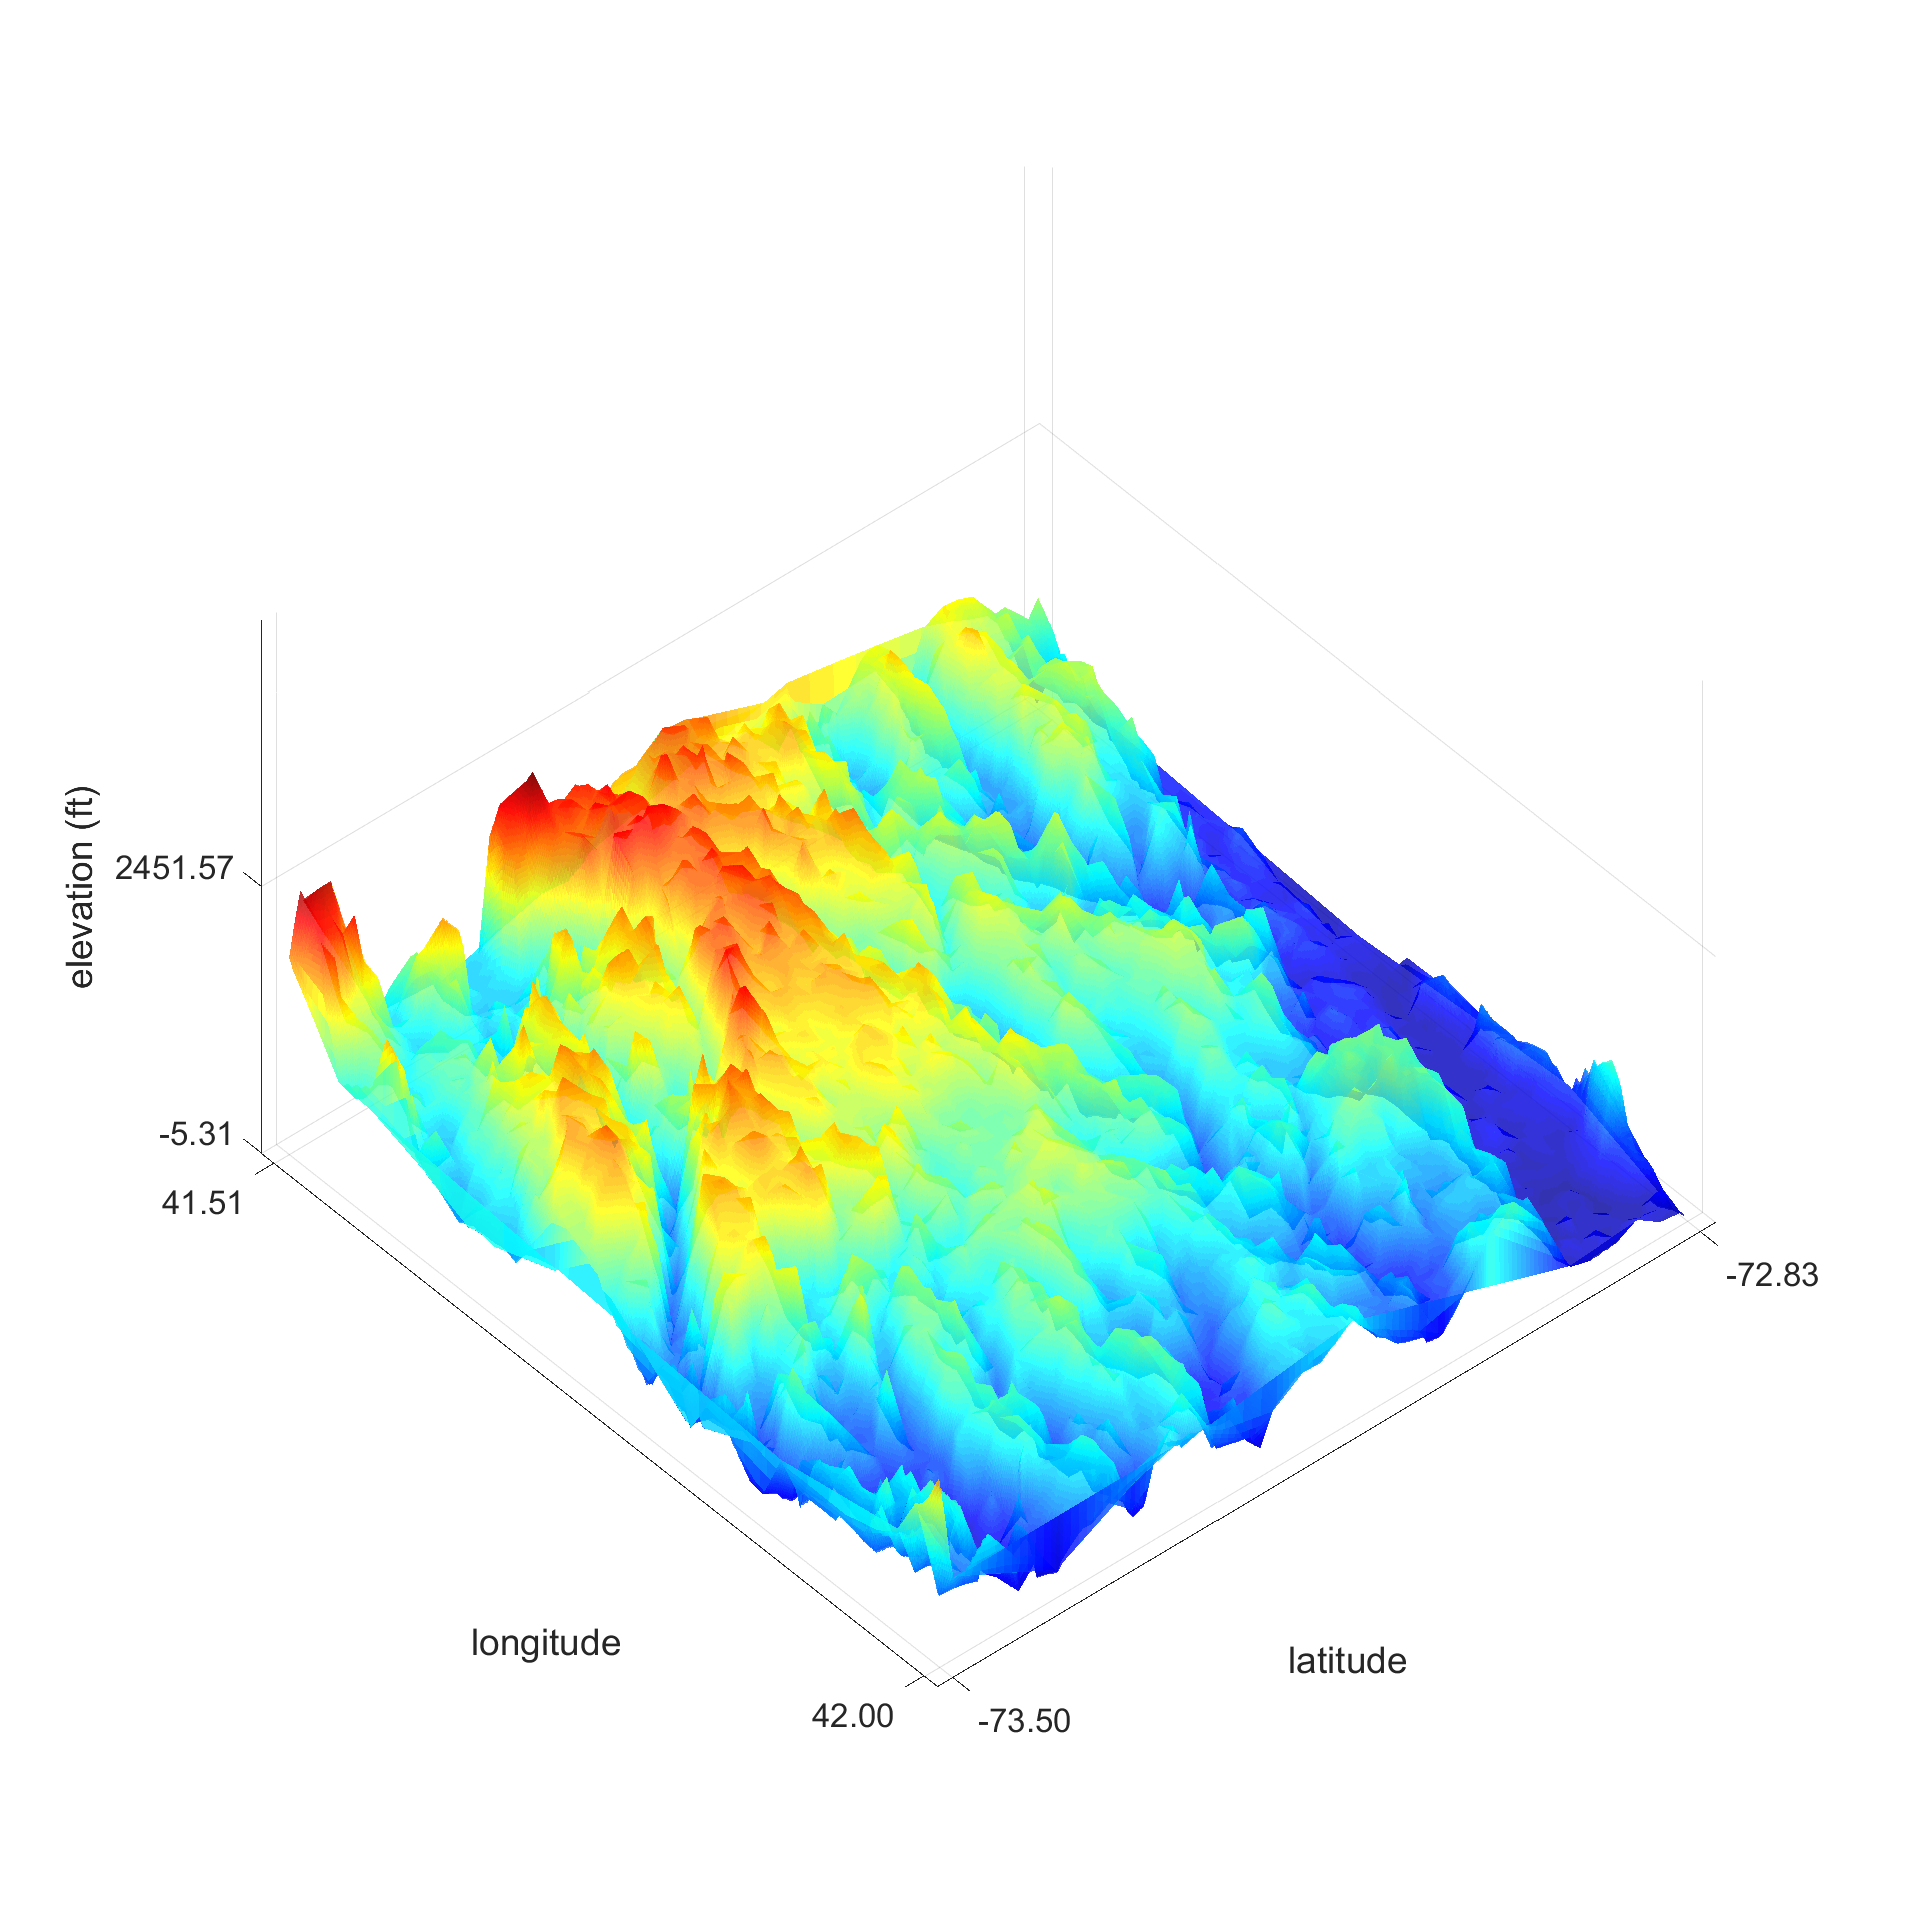
\includegraphics[width=2.5in]{figure/gtruth3d}
	\caption{Elevation map of some region in Connecticut (the ground truth).} 
	\label{fig:fig1}
\end{figure}

%\begin{figure}
%	\centering
%	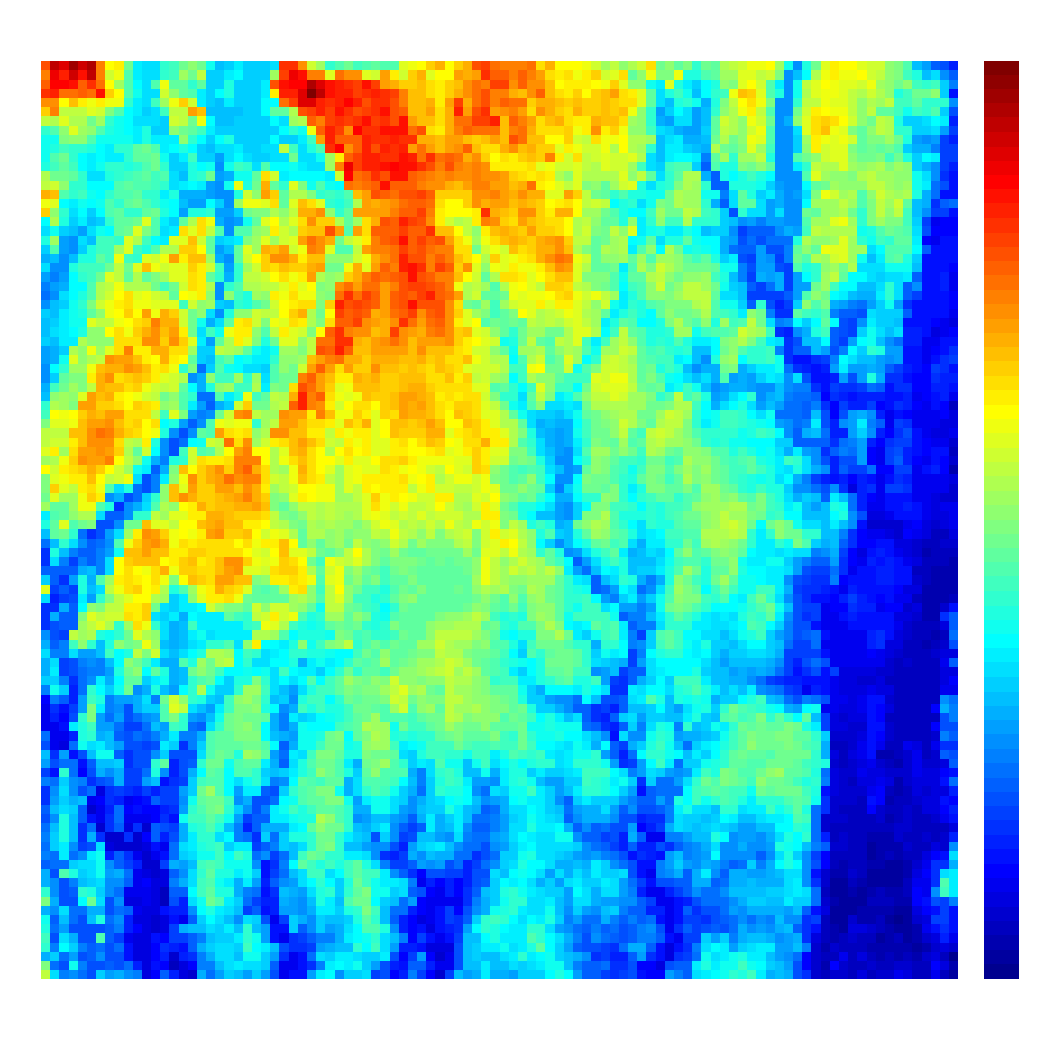
\includegraphics[width=1.6in]{figure/init}
%	\caption{Expected target intensity for an arbitrary distribution (the ground truth)} 
%	\label{fig:fig1}
%\end{figure}
\begin{figure}
		\centering
  	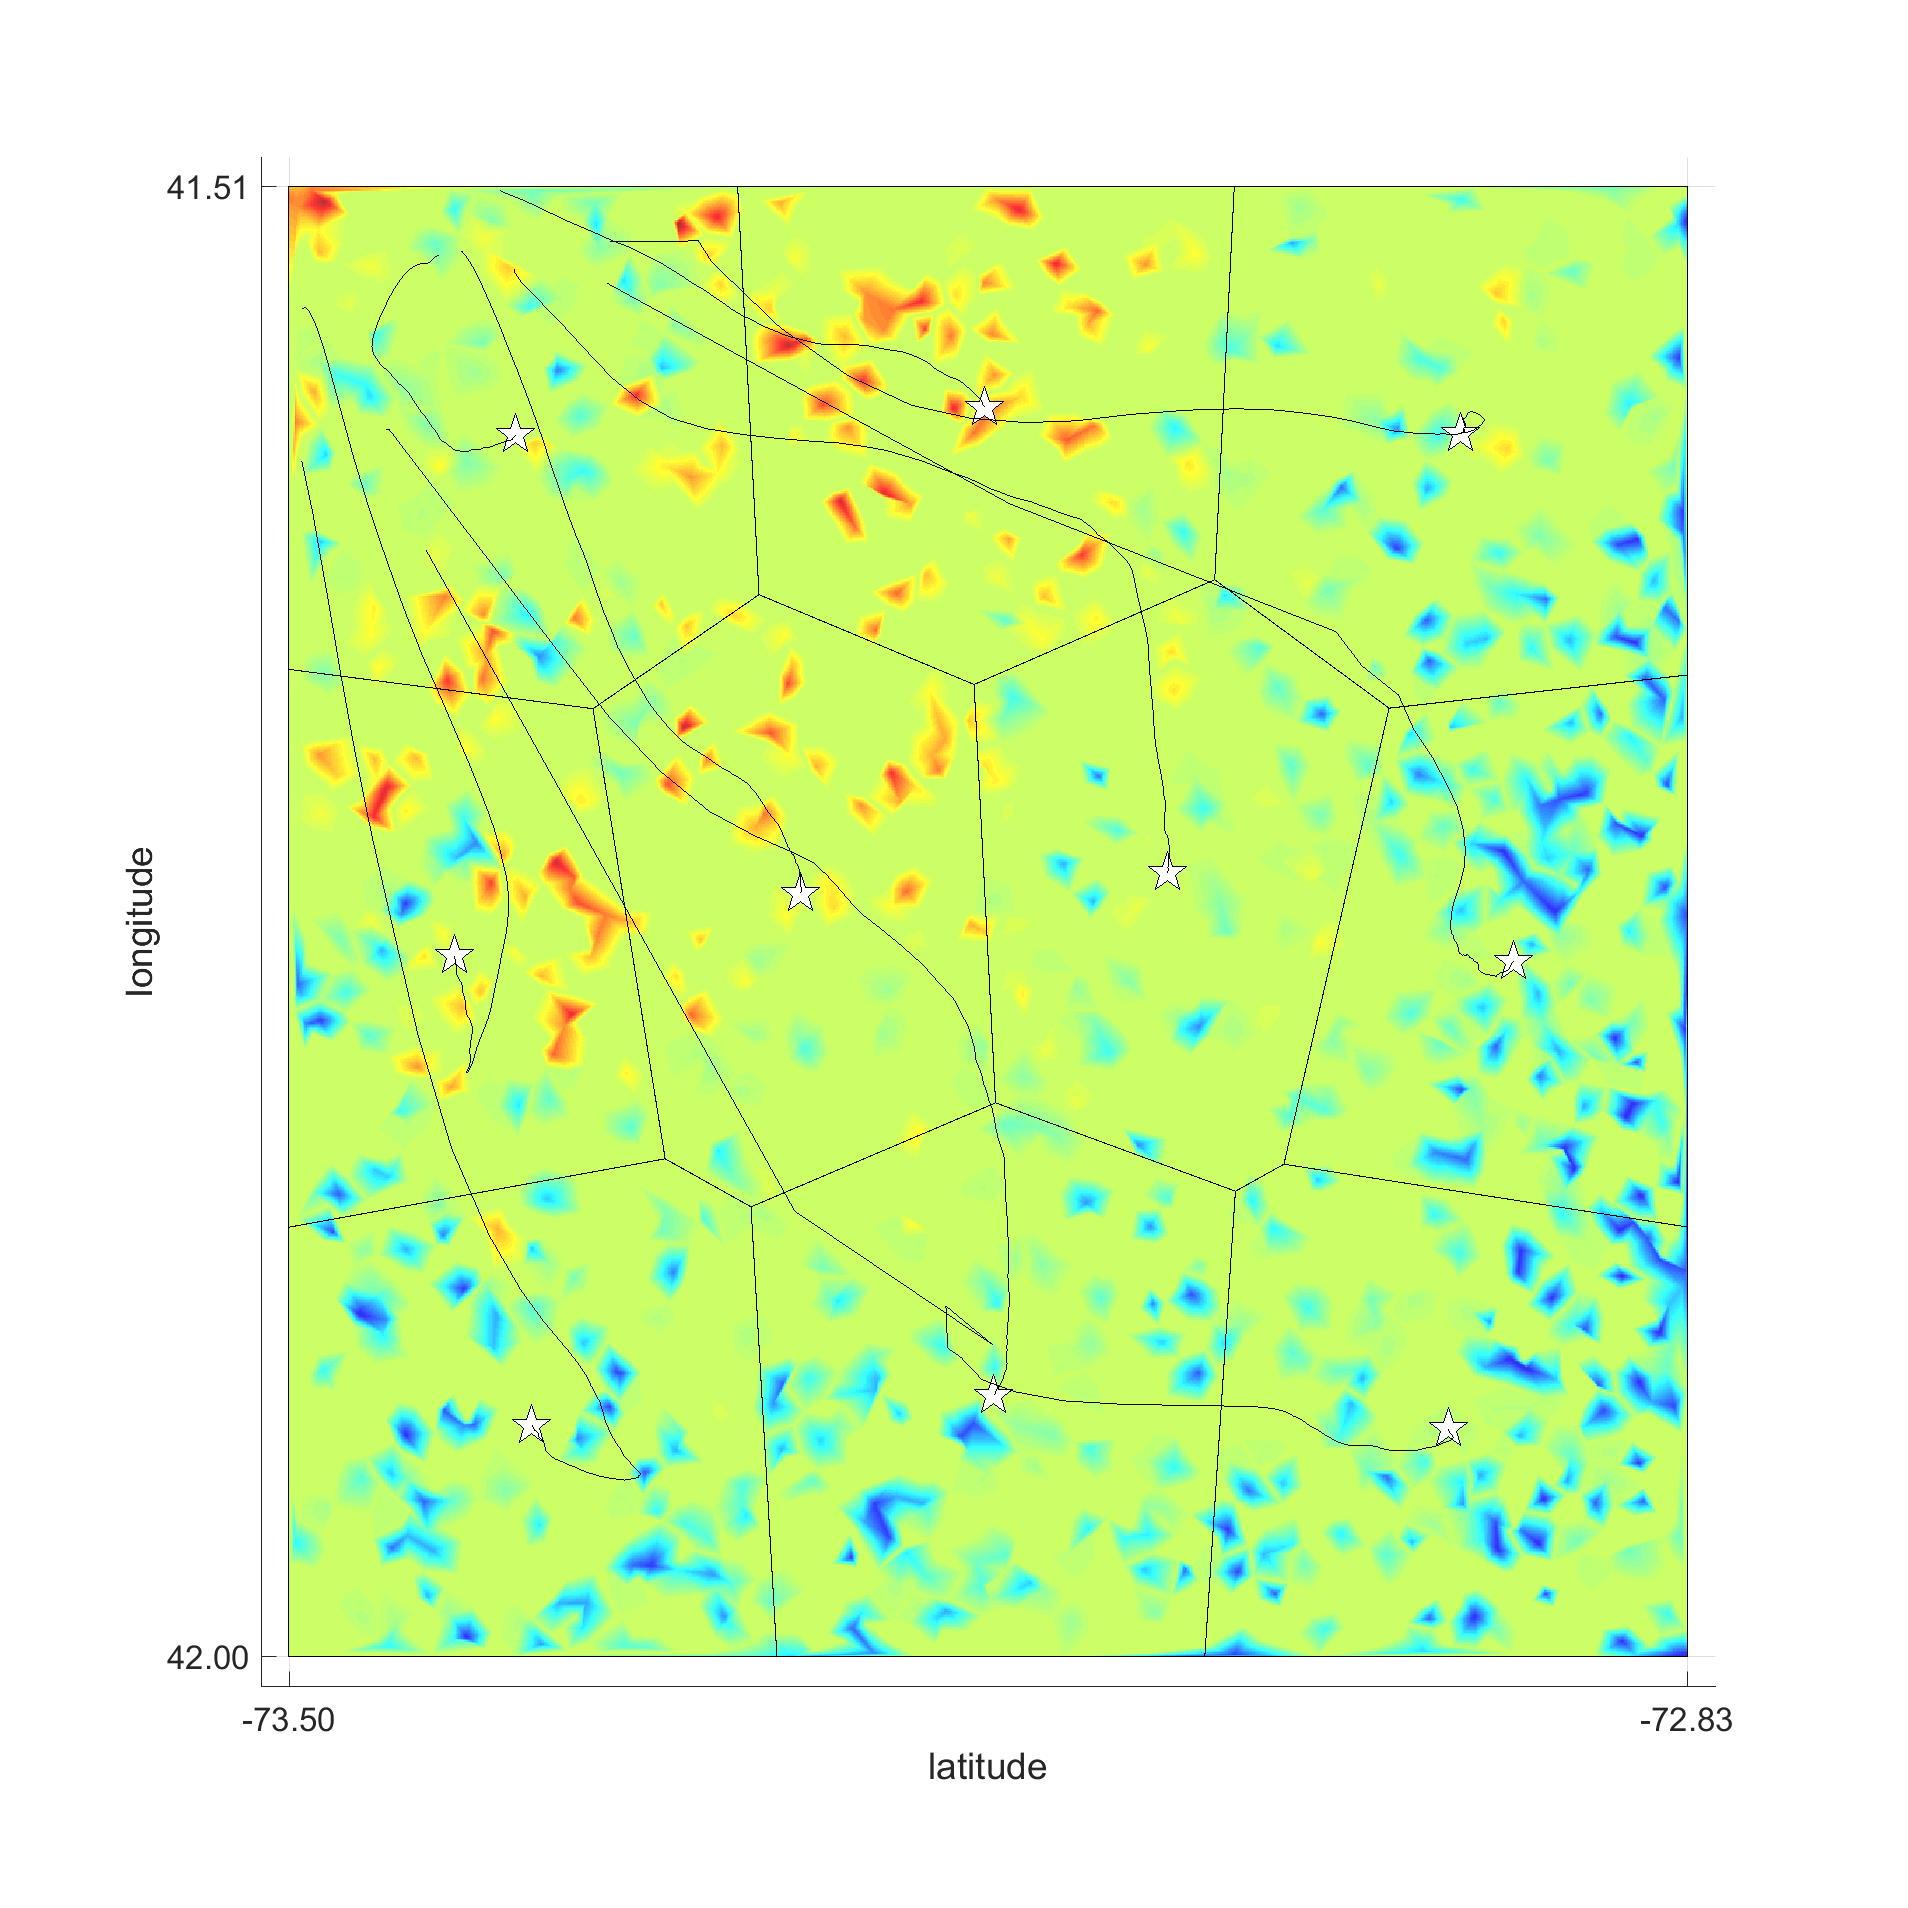
\includegraphics[width=1.55in]{figure/order1deploy2d}
  	  	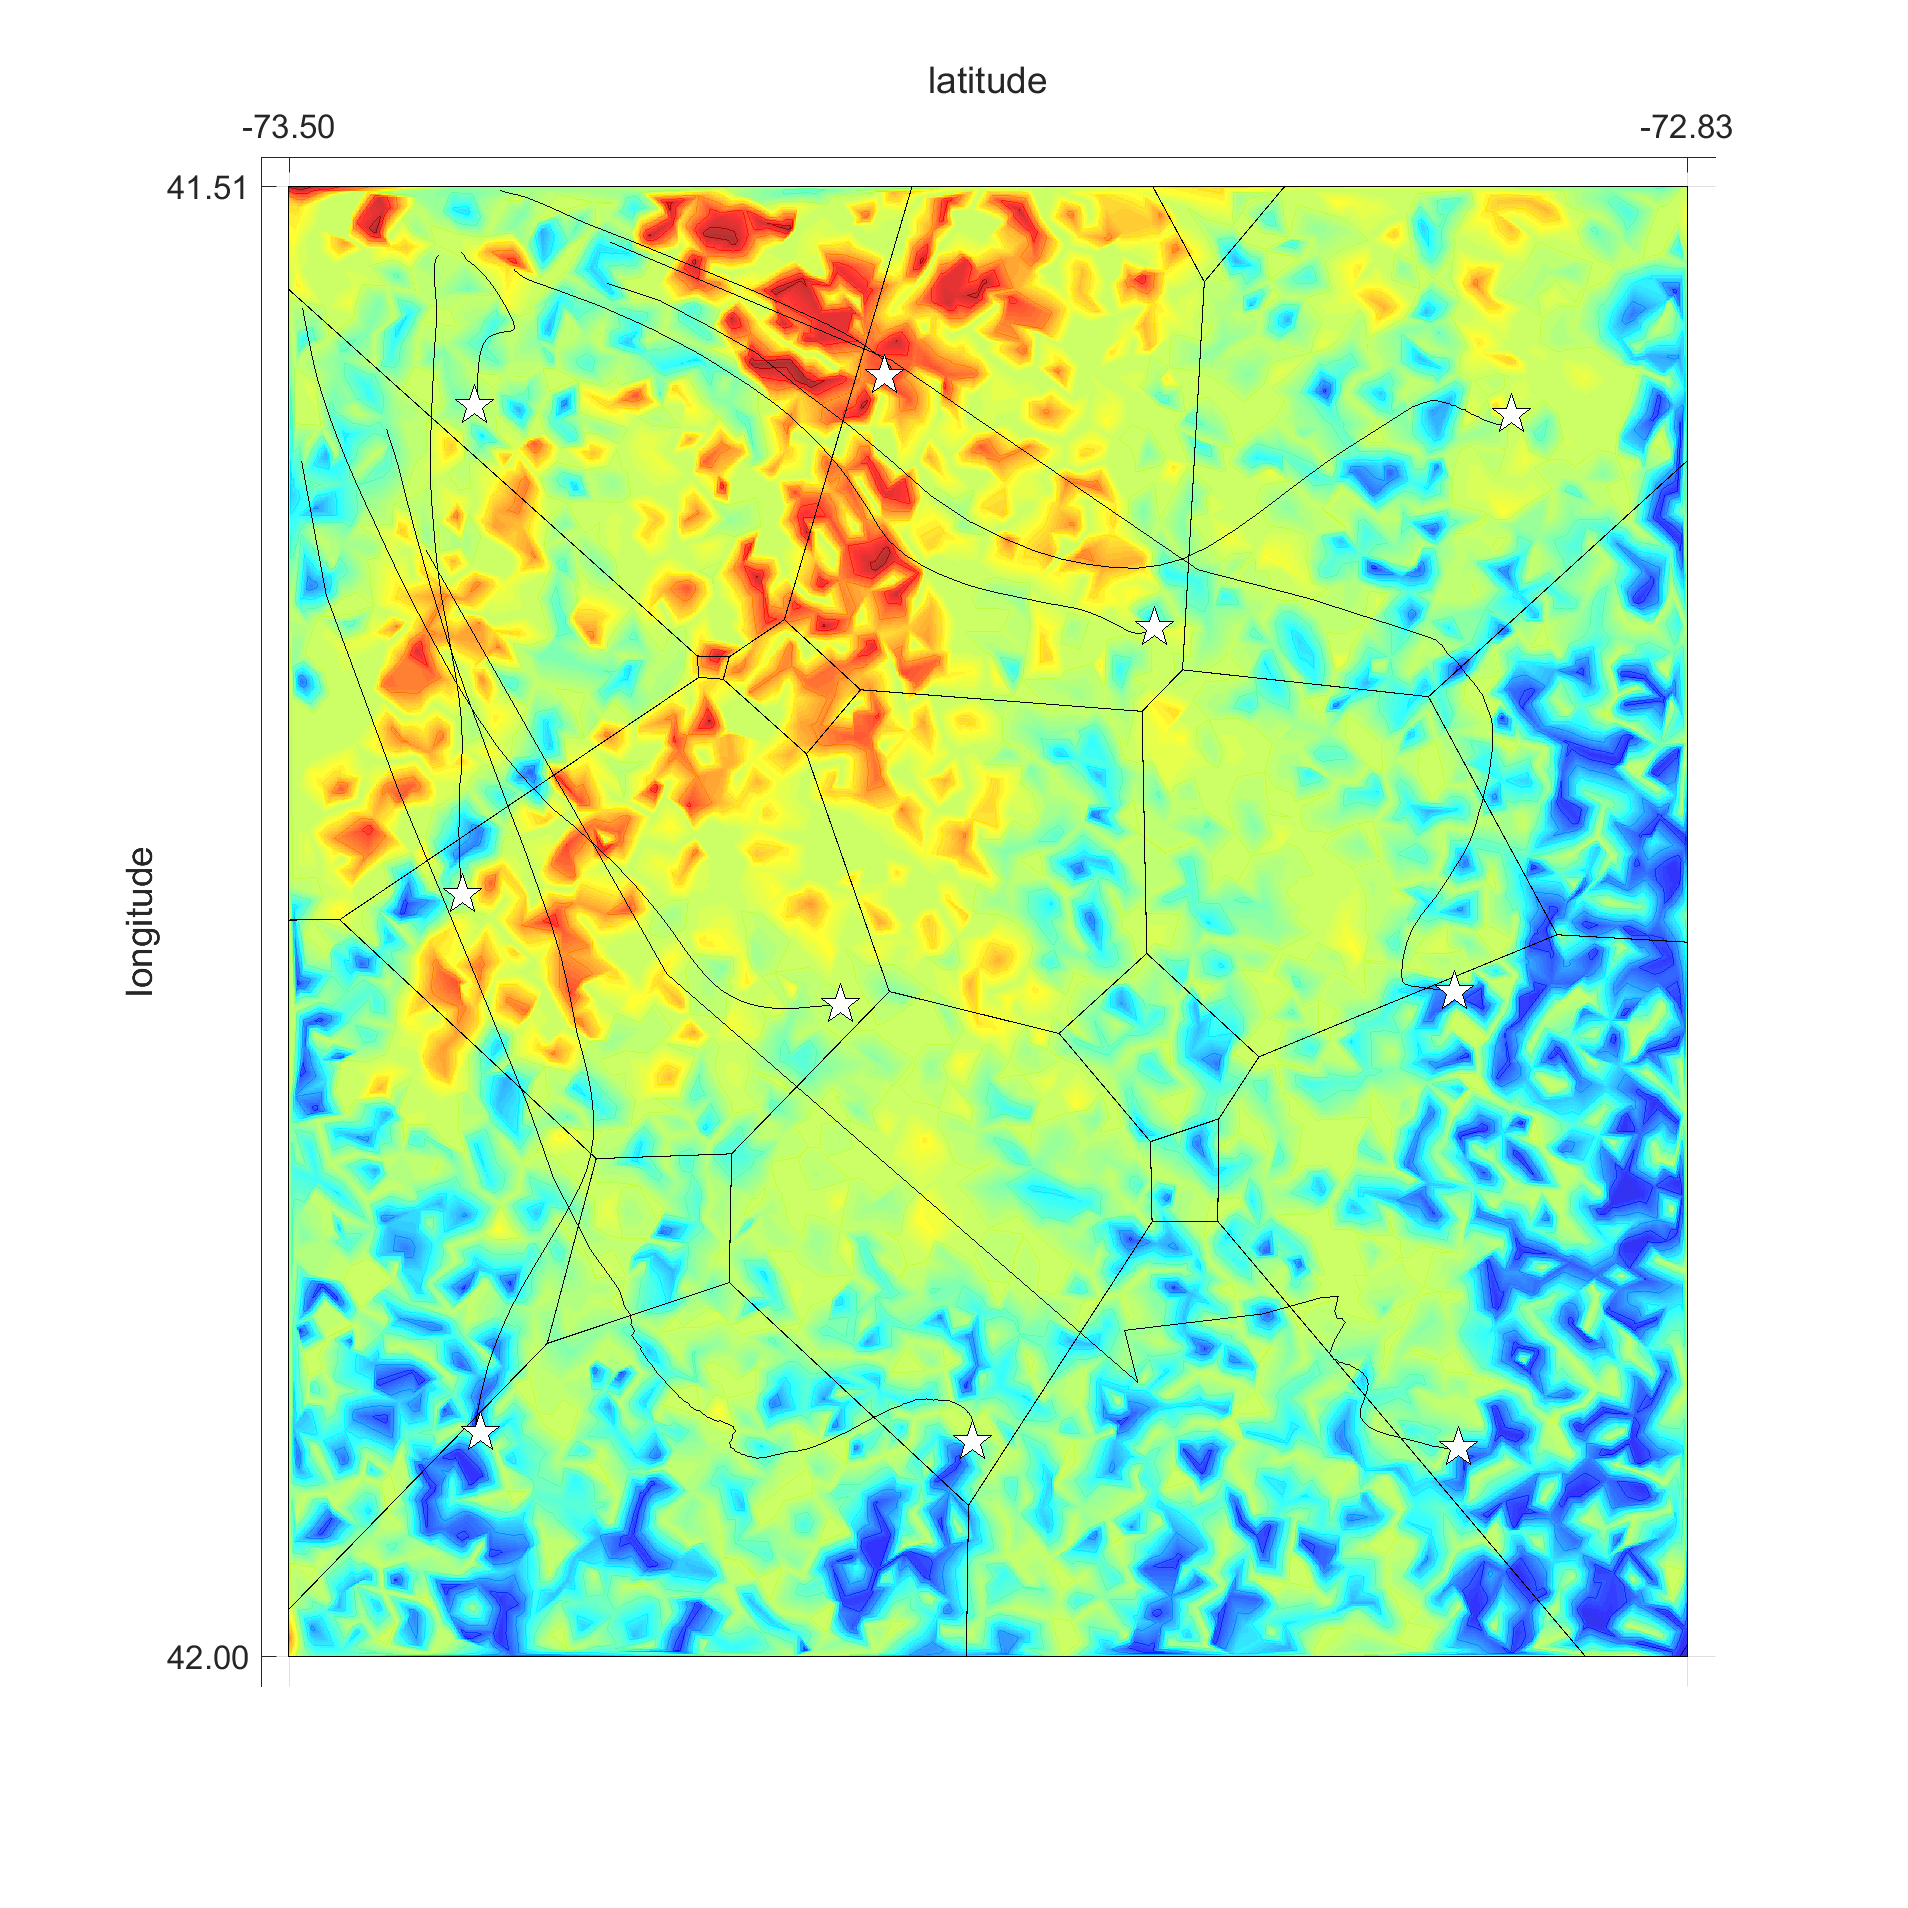
\includegraphics[width=1.55in]{figure/order2deploy2d}
%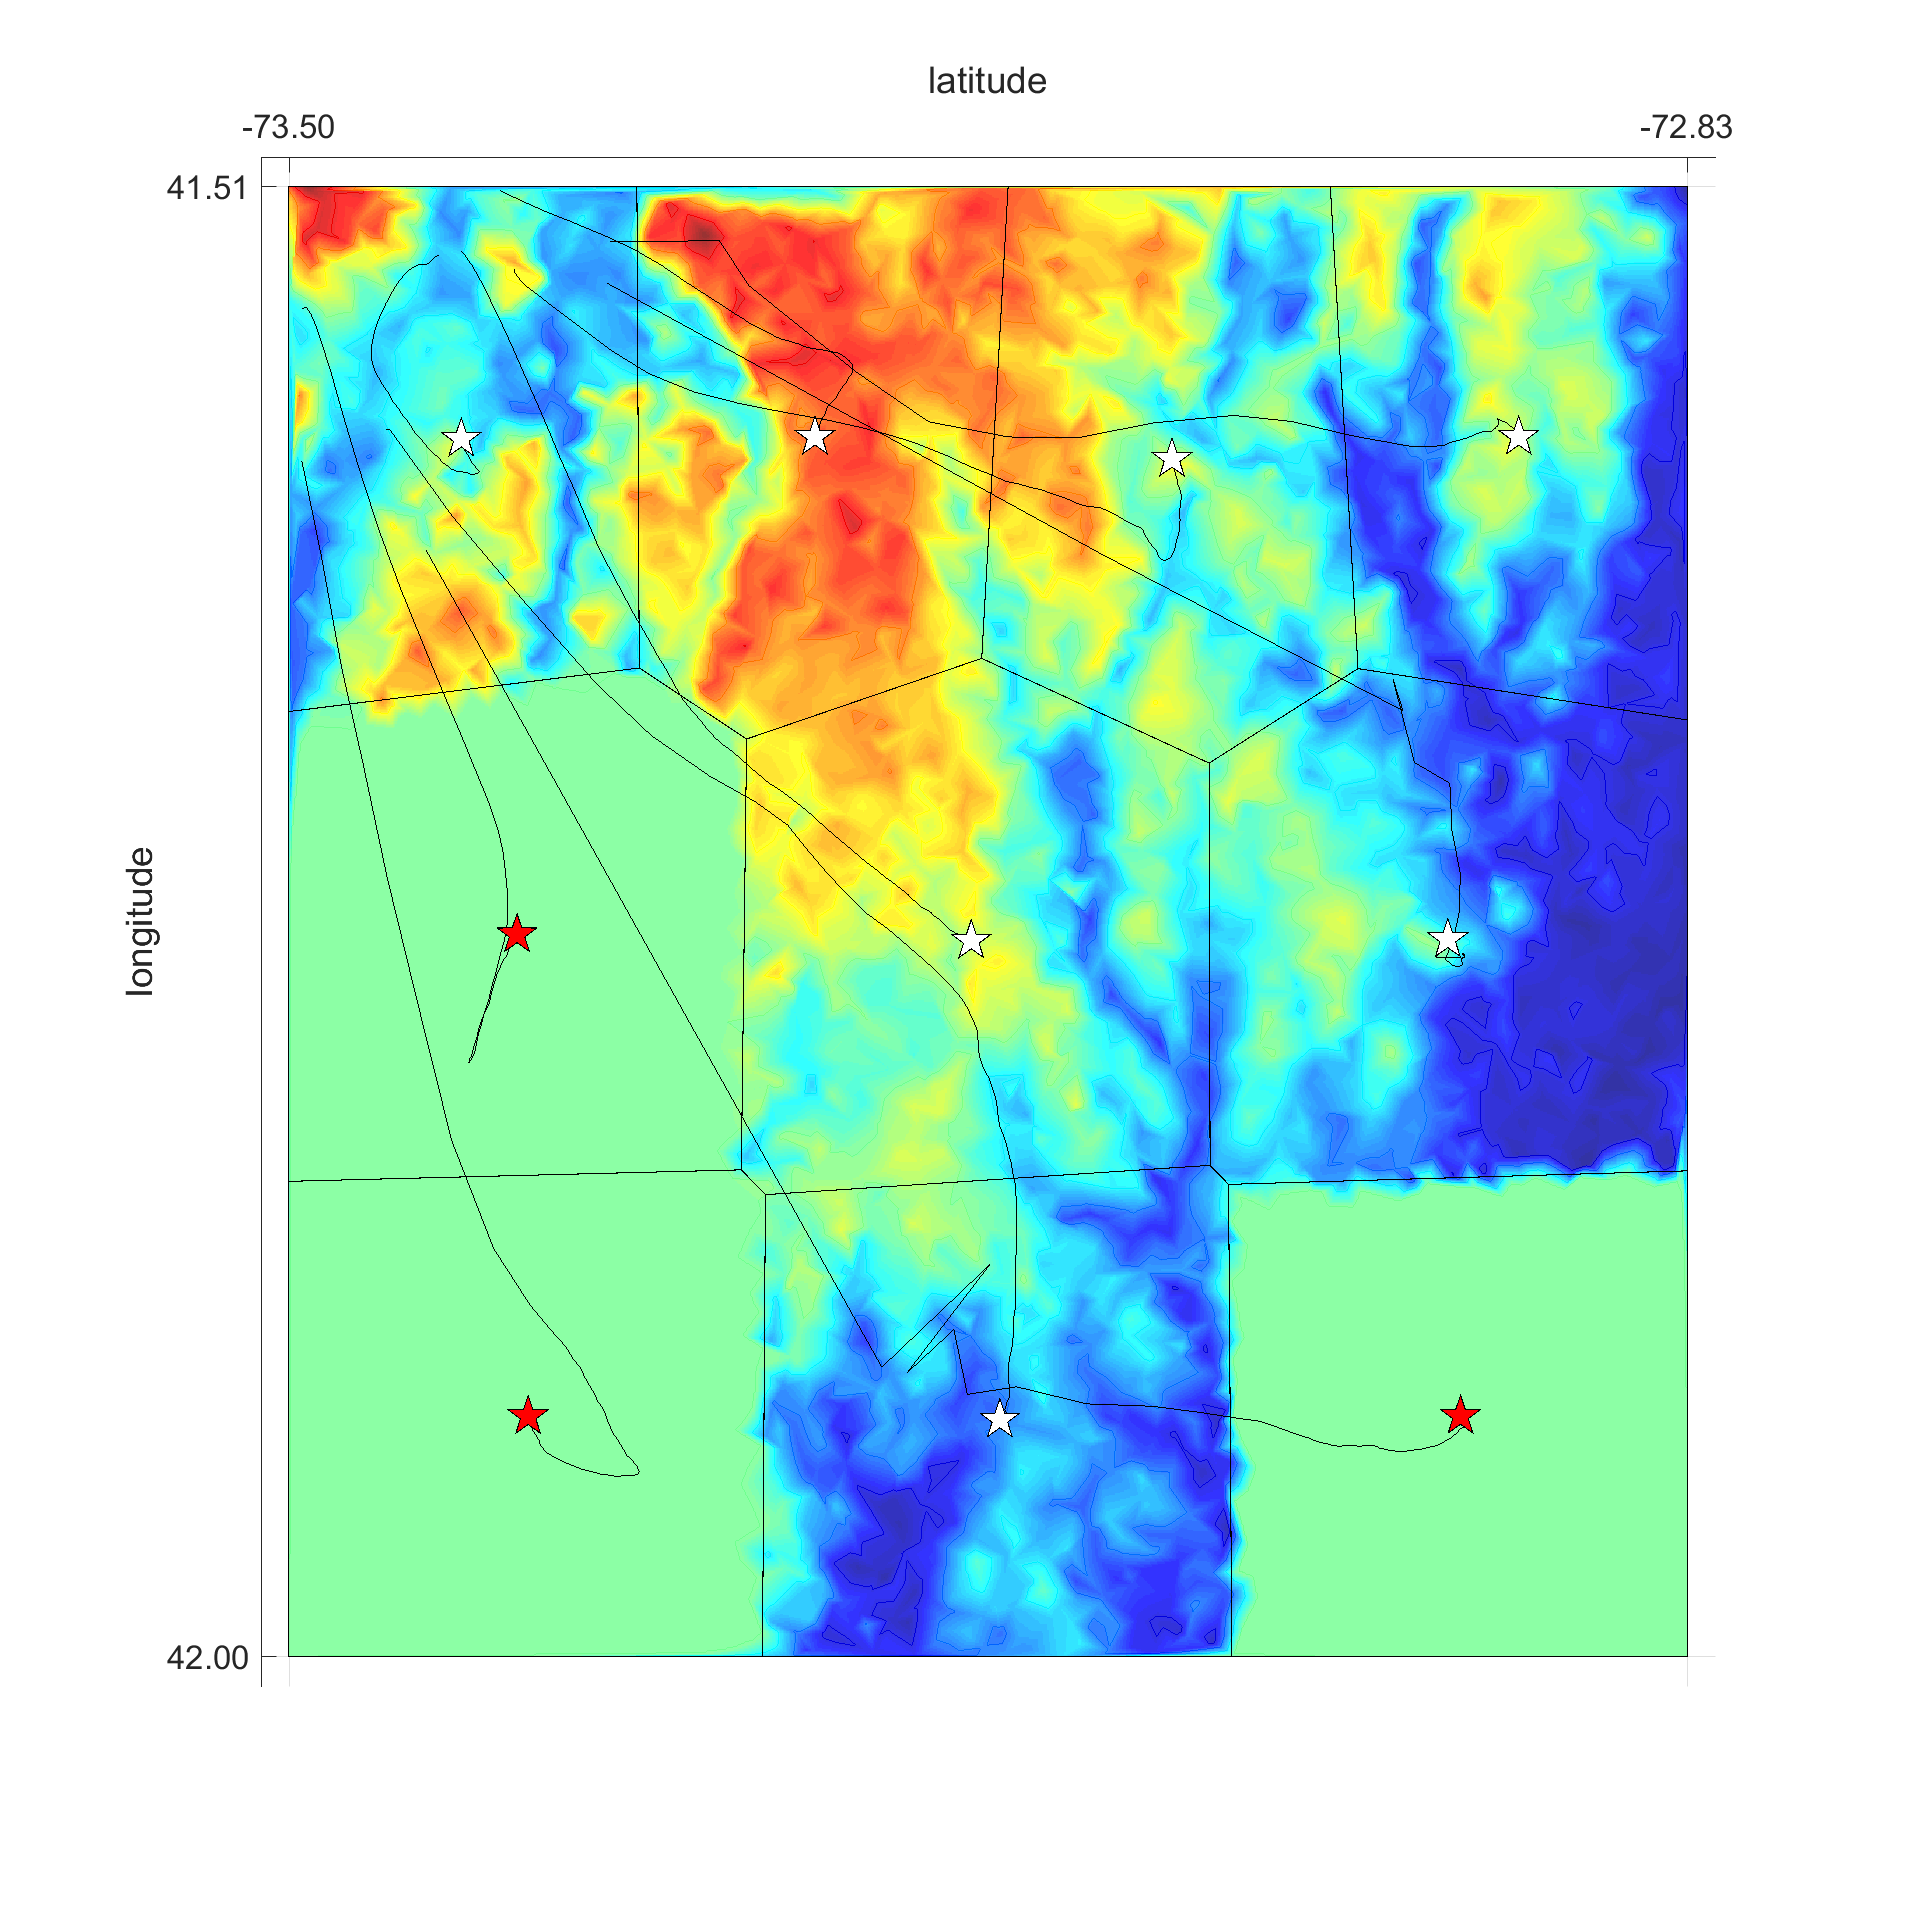
\includegraphics[width=1.57in]{figure/final_config_order1_fault}
	%	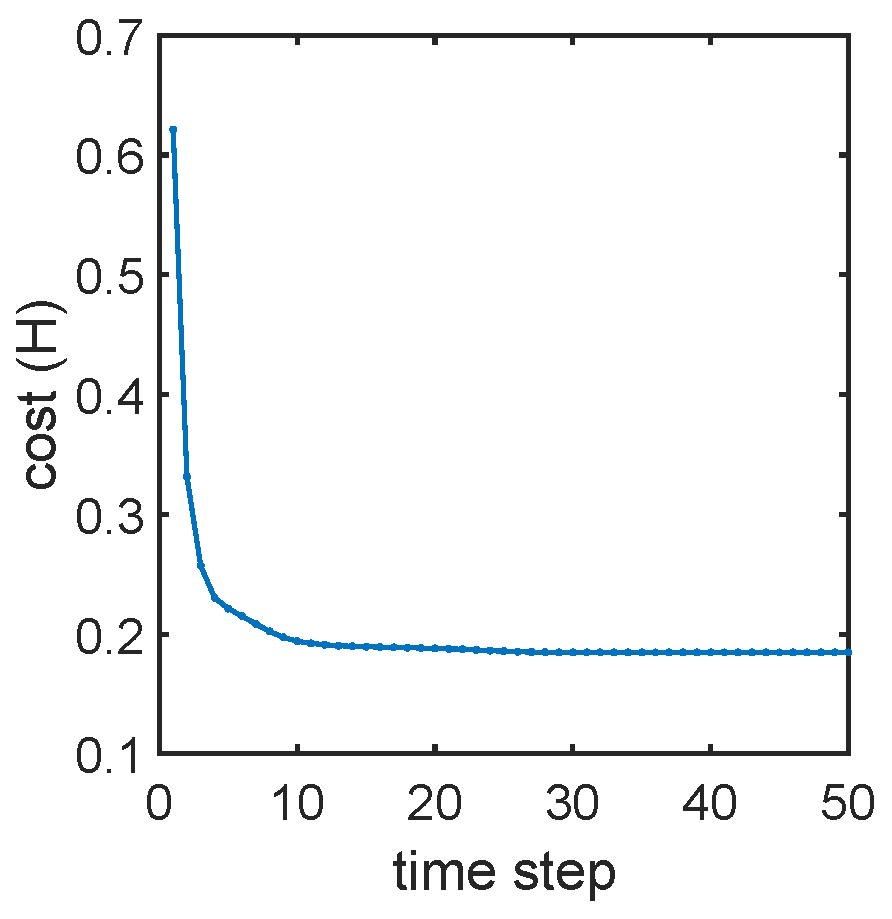
\includegraphics[width=3.4in]{figure/init_10_deploy_cmd2}
	\caption{One-time deployment with non-robust (left) and robust ($k=2$) (right) overlaid with map at $t=1$ (lines: gradient descent flow, stars: positions of robots, polygons: partition).}
	\label{fig:fig2}
\end{figure}

\begin{figure}
	\centering
	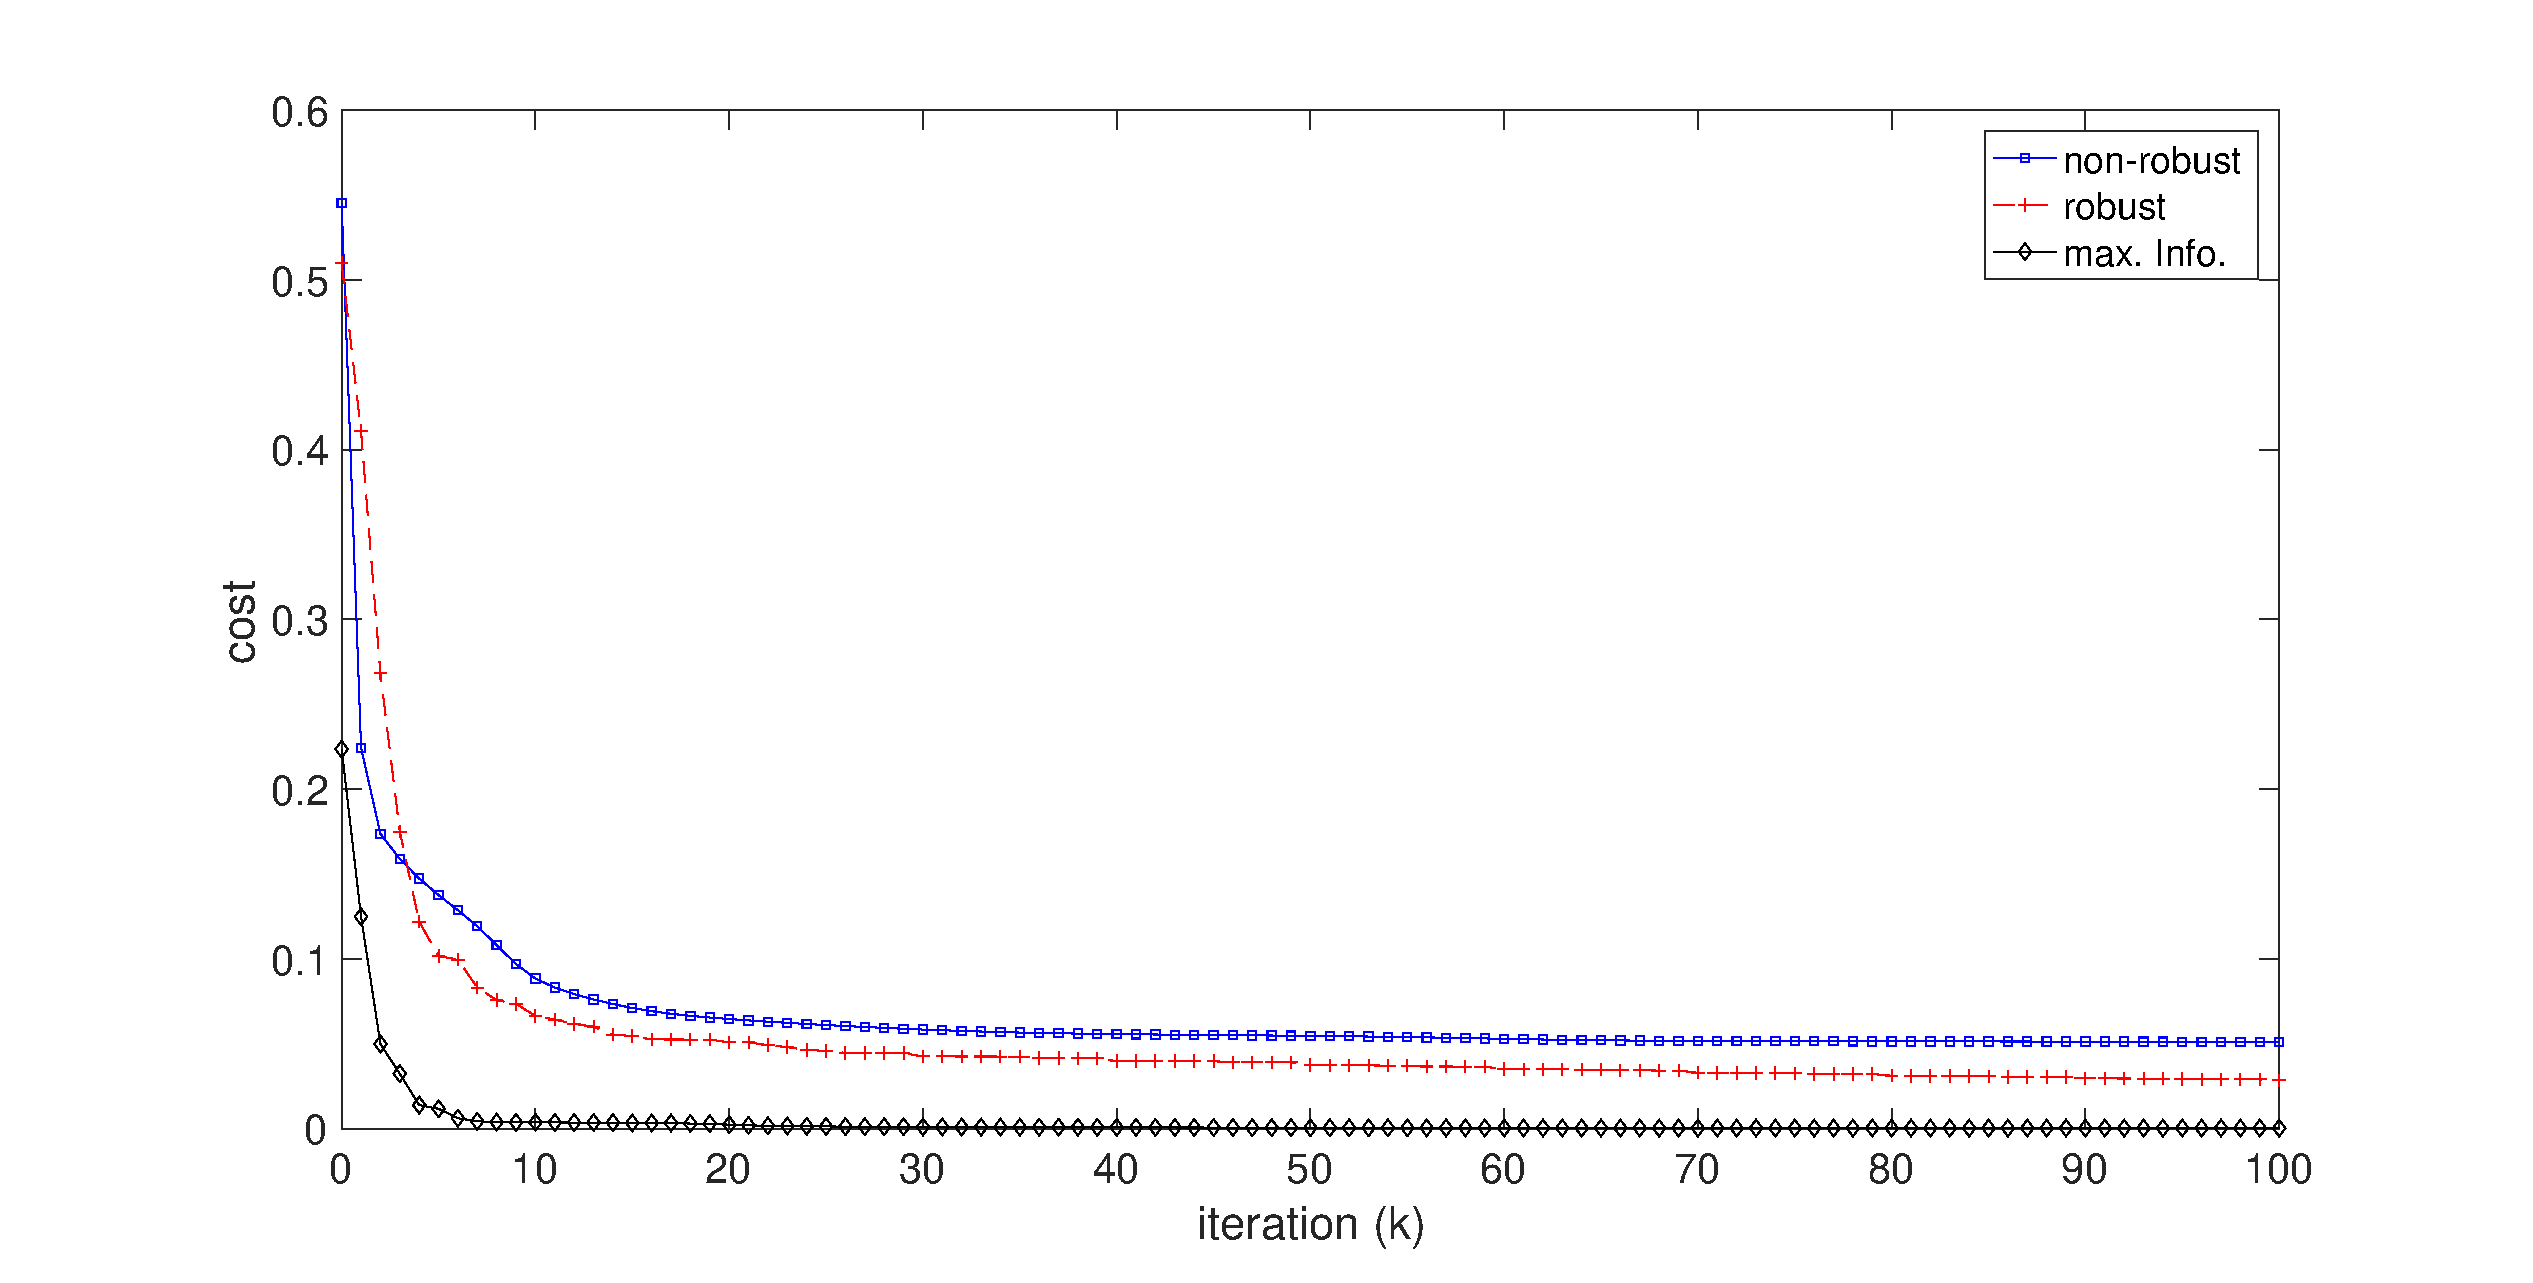
\includegraphics[width=2.9in]{figure/cost_comp1}
	%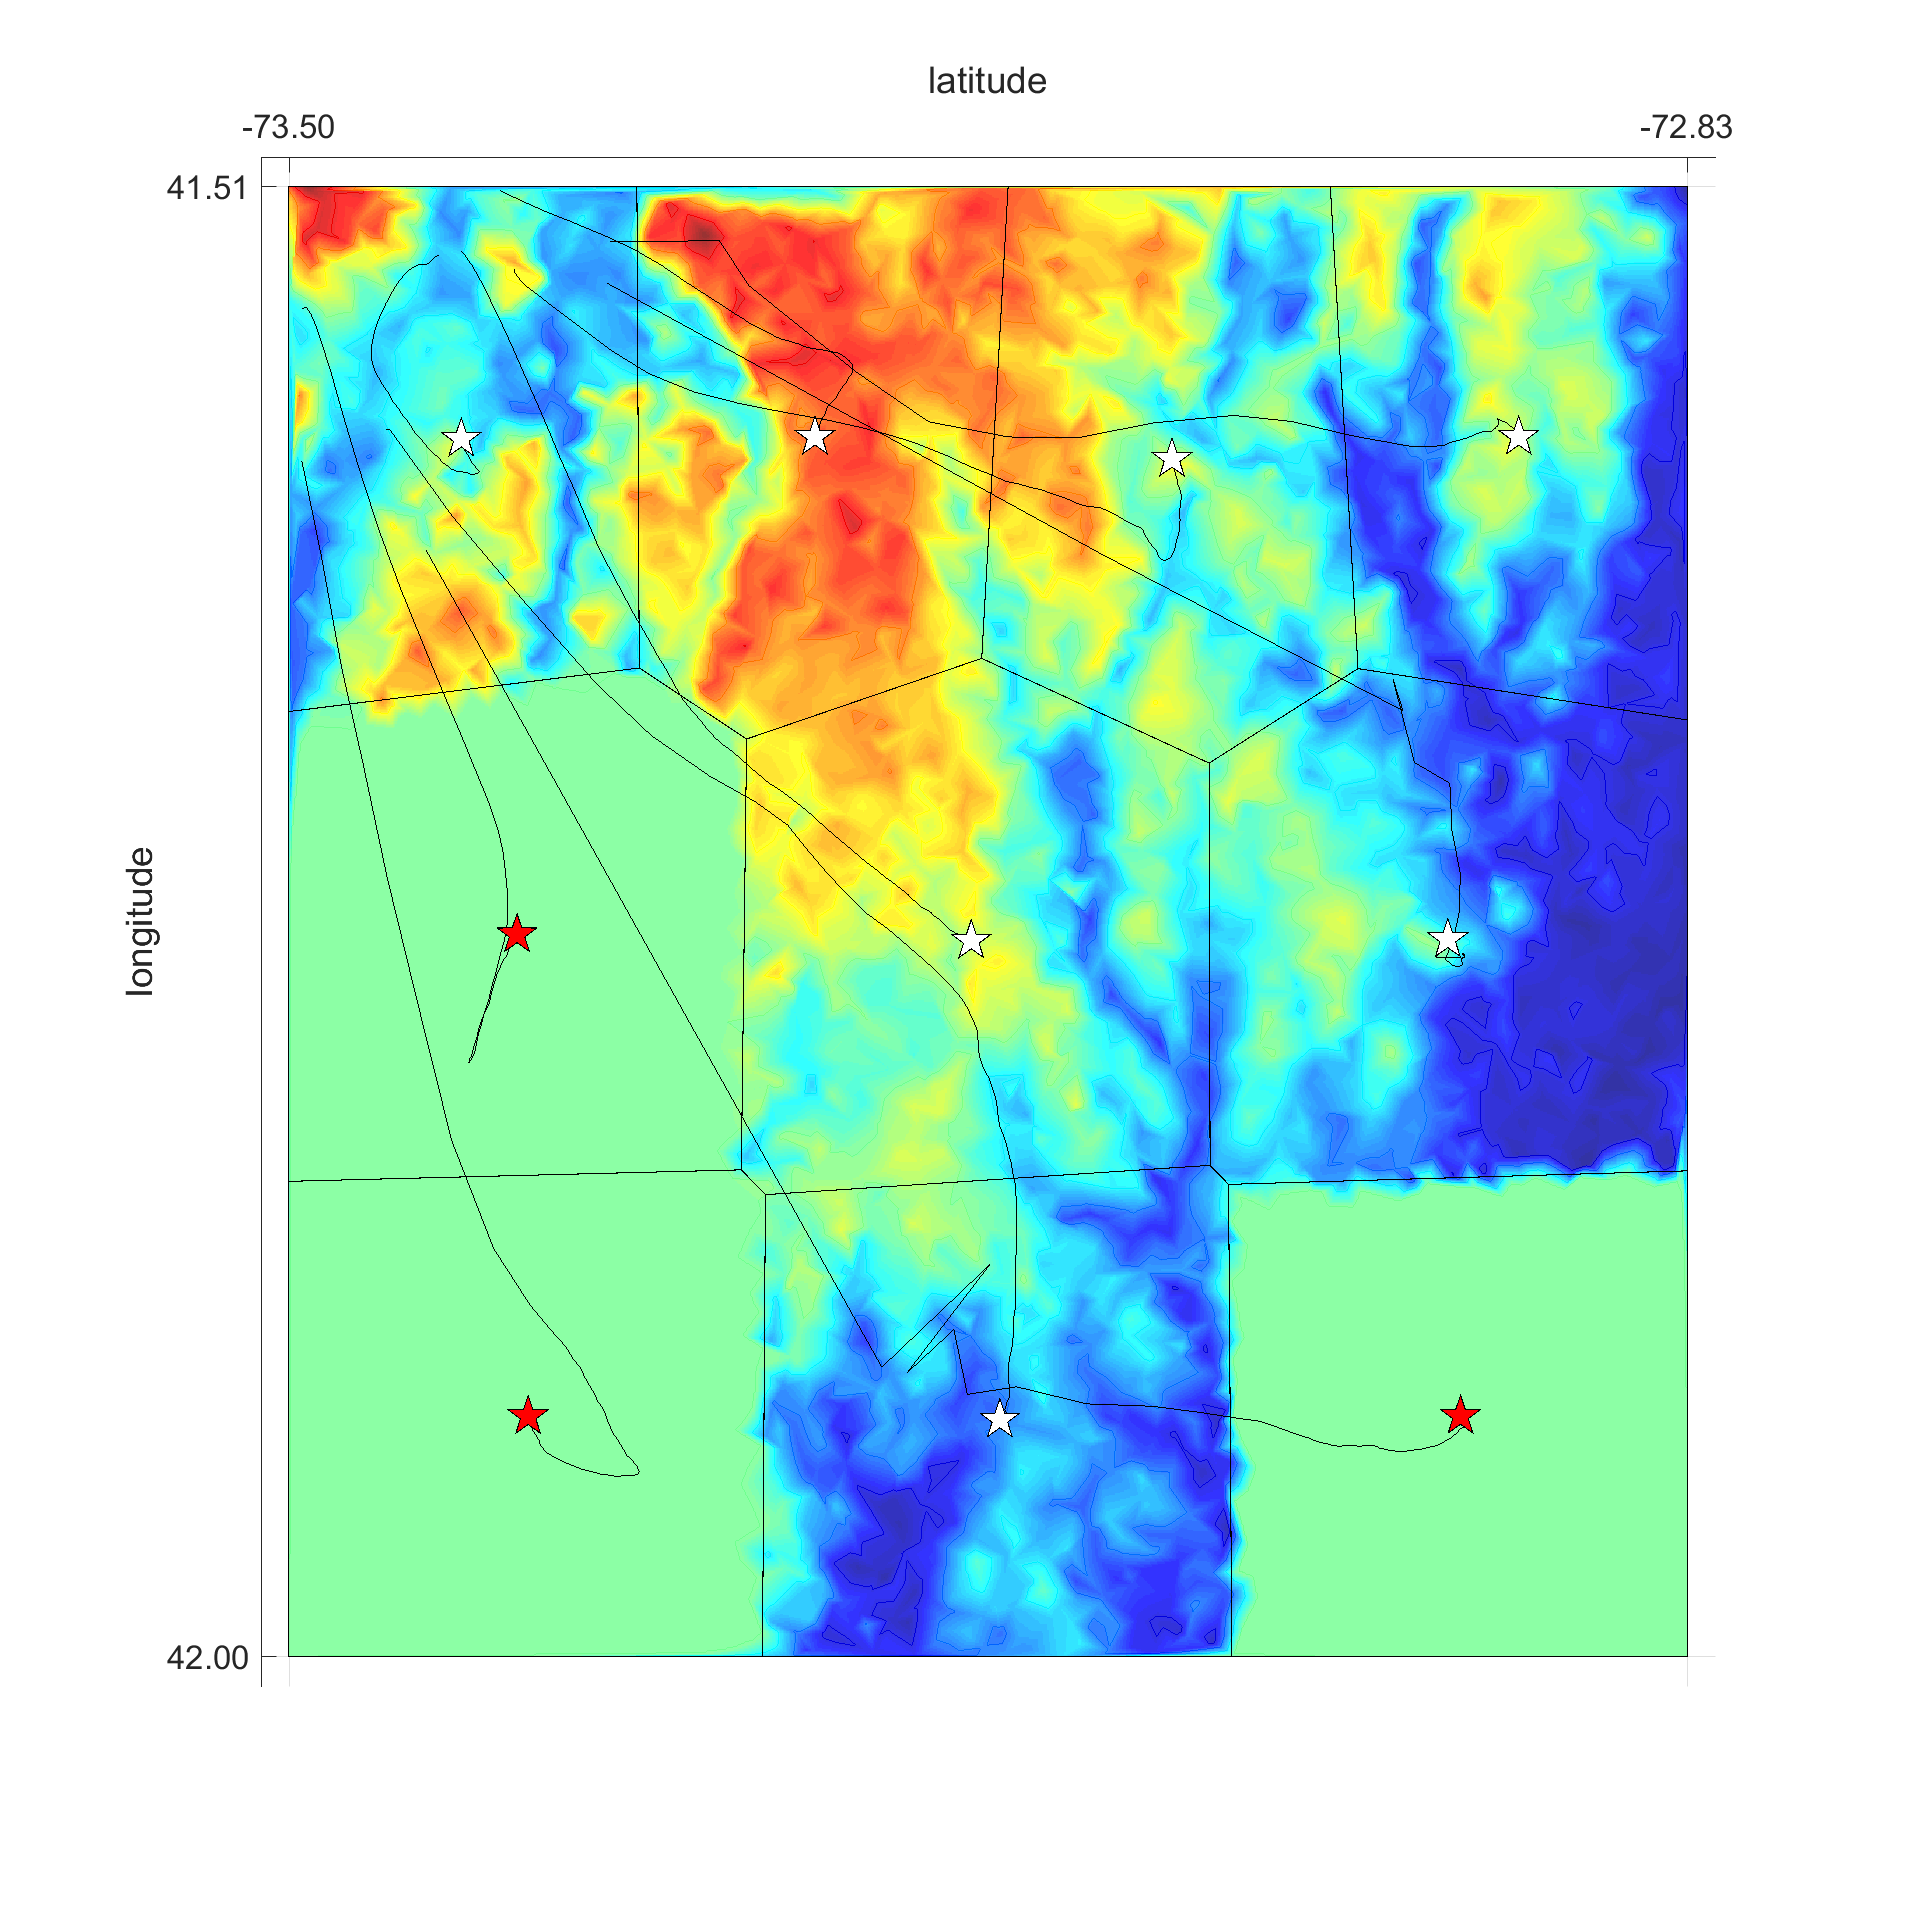
\includegraphics[width=1.57in]{figure/final_config_order1_fault}
	%	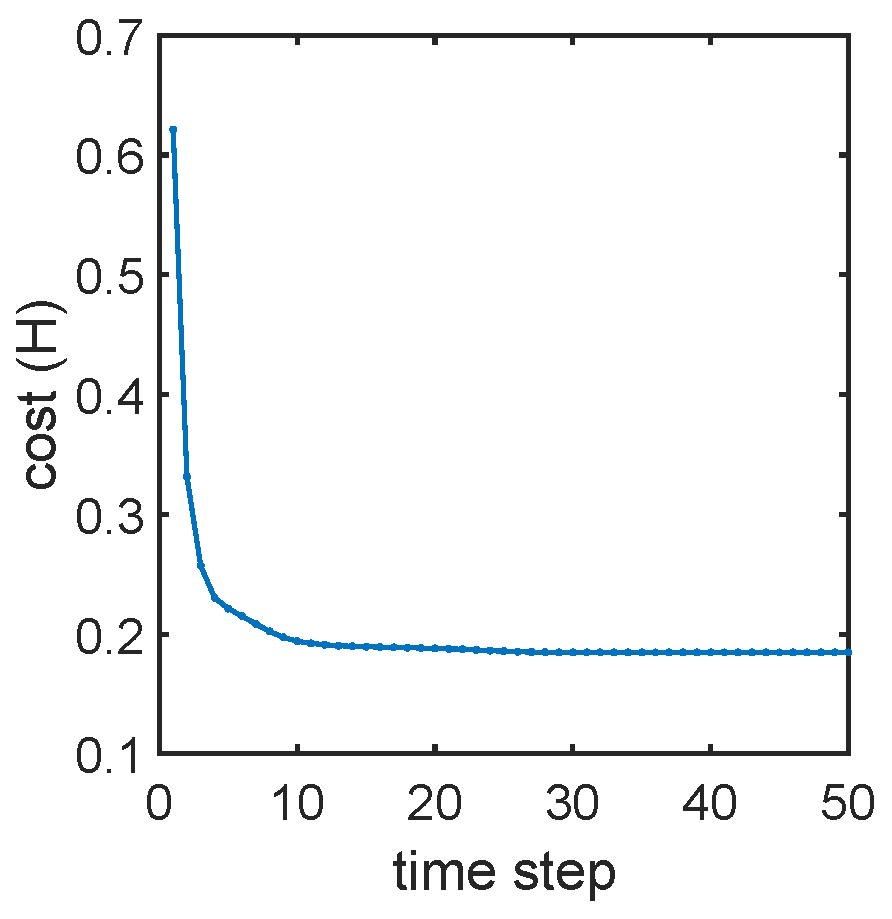
\includegraphics[width=3.4in]{figure/init_10_deploy_cmd2}
	\caption{Convergence test for one-time deployment with different methods.}
	\label{fig:fig0}
\end{figure}


%\begin{figure}
%	\centering
%	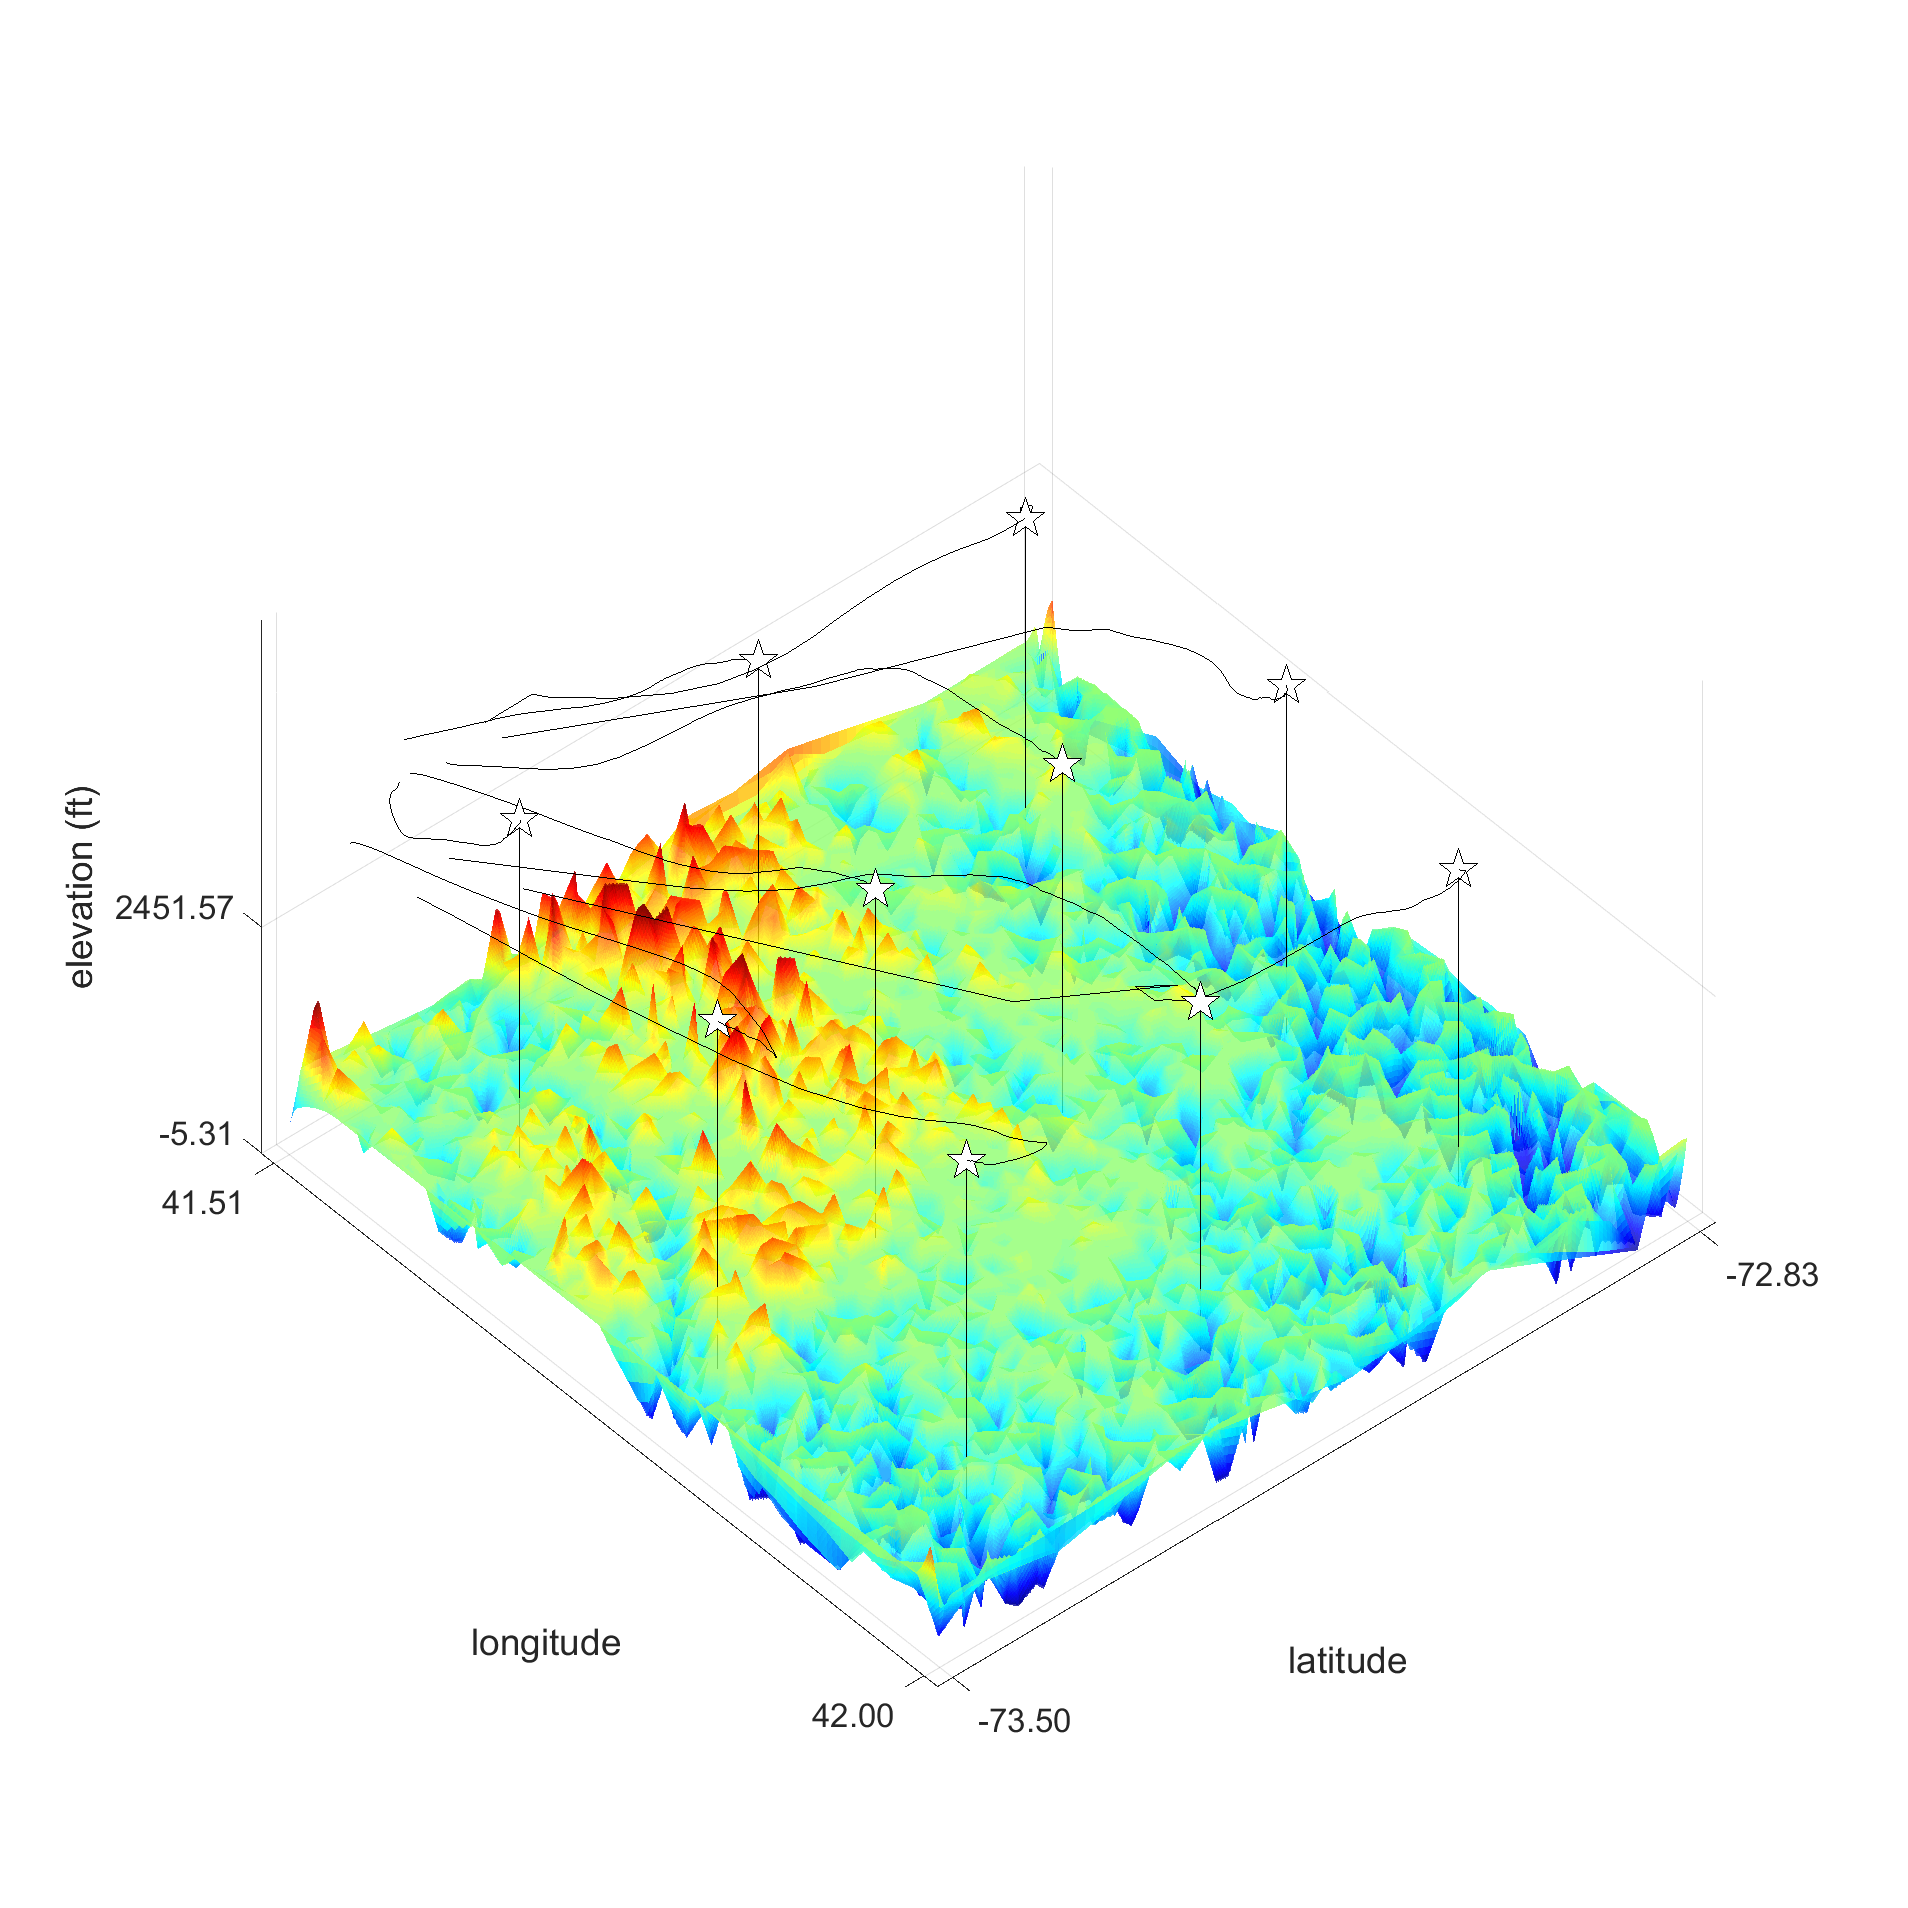
\includegraphics[width=1.1in]{figure/order1deploy3d}
%	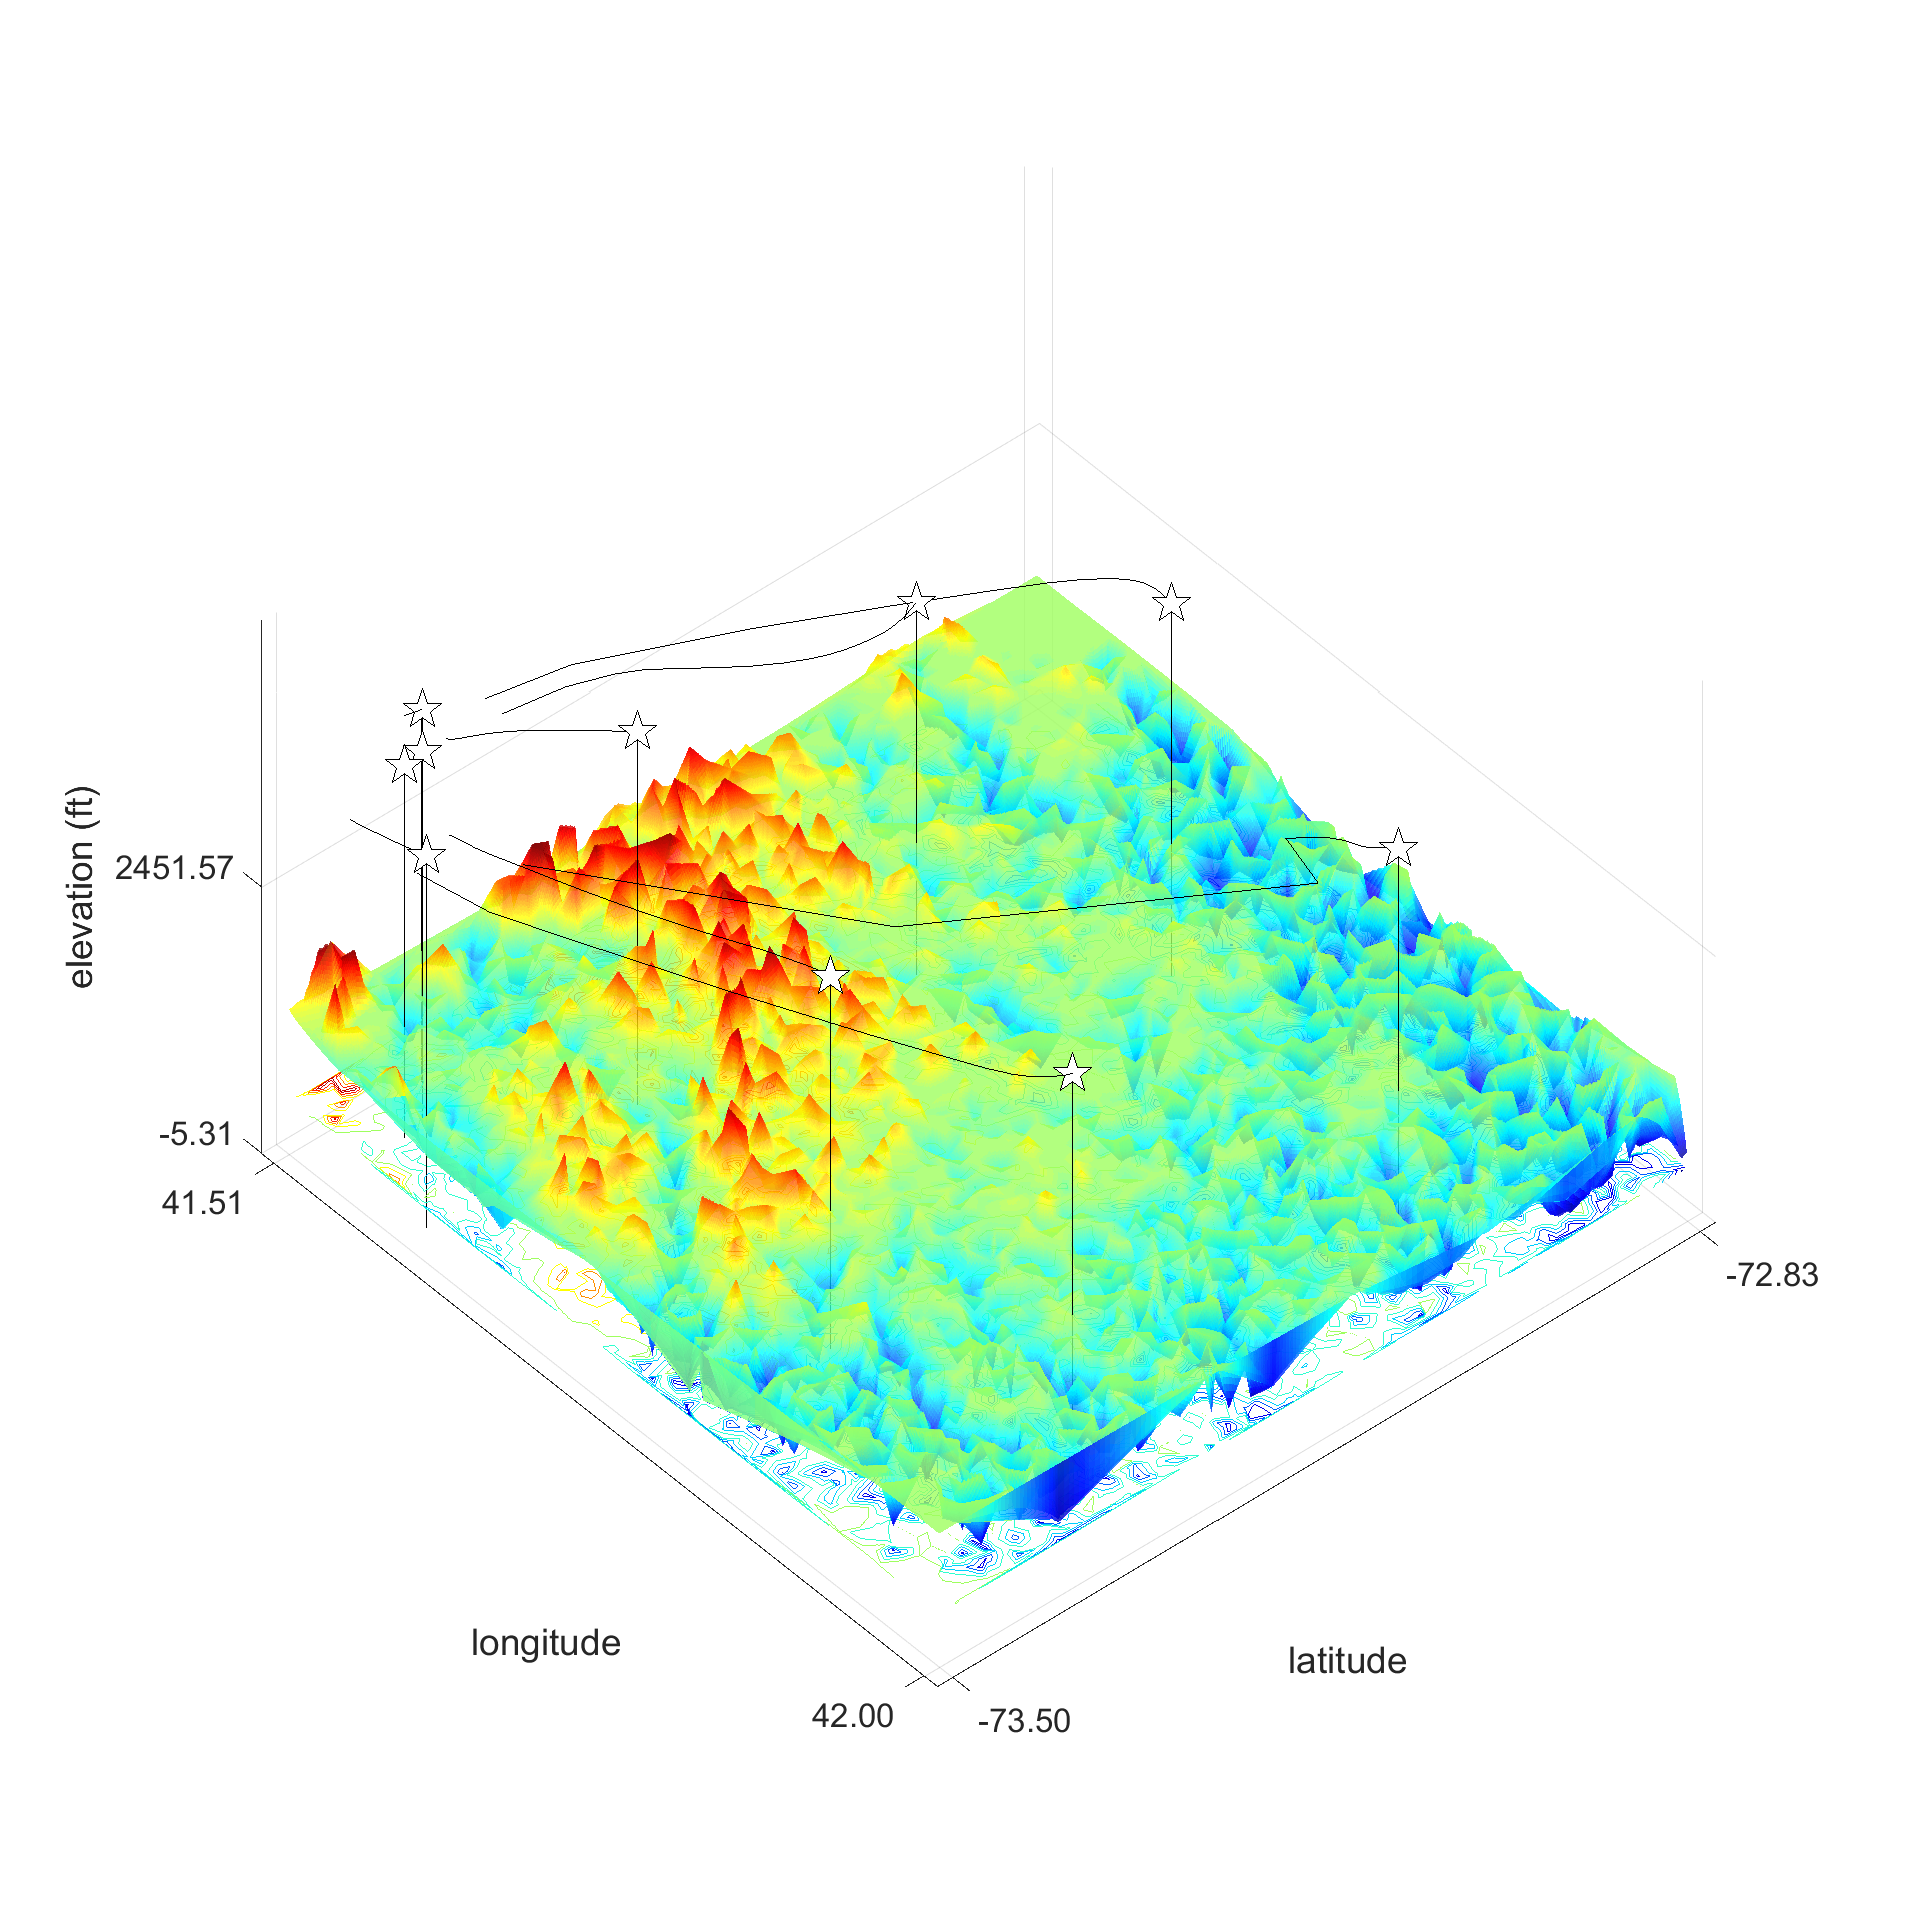
\includegraphics[width=1.1in]{figure/order2deploy3d}
%%	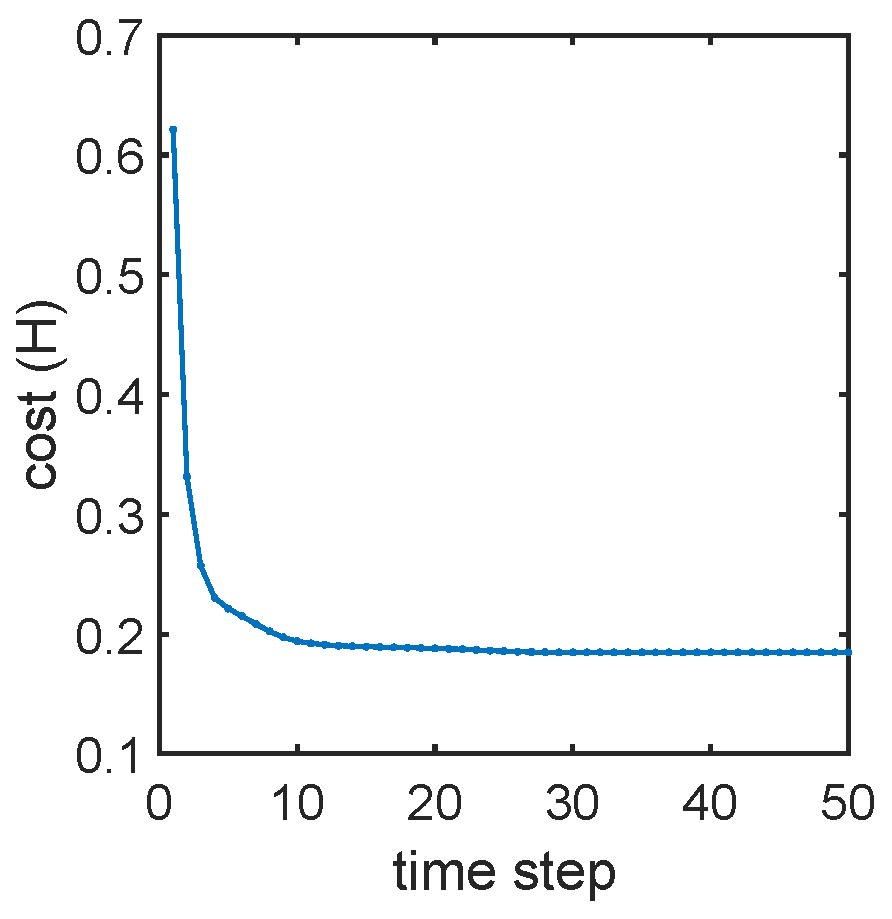
\includegraphics[width=3.4in]{figure/init_10_deploy_cmd2}
%	\caption{One-time deployment with $k=1$, (a) cost change during Algorithm 1 ($0^{\textup{th}}-1^{\textup{st}}$ step) , (b) optimal path respecting unicycle kinematic constraint (circles: initial positions, stars: target positions, polygons: partition)}
%	\label{fig:fig2}
%\end{figure}
\begin{figure*}
%	\centering
%	 \begin{subfigure}[b]{0.165\textwidth}
	 	\centering
		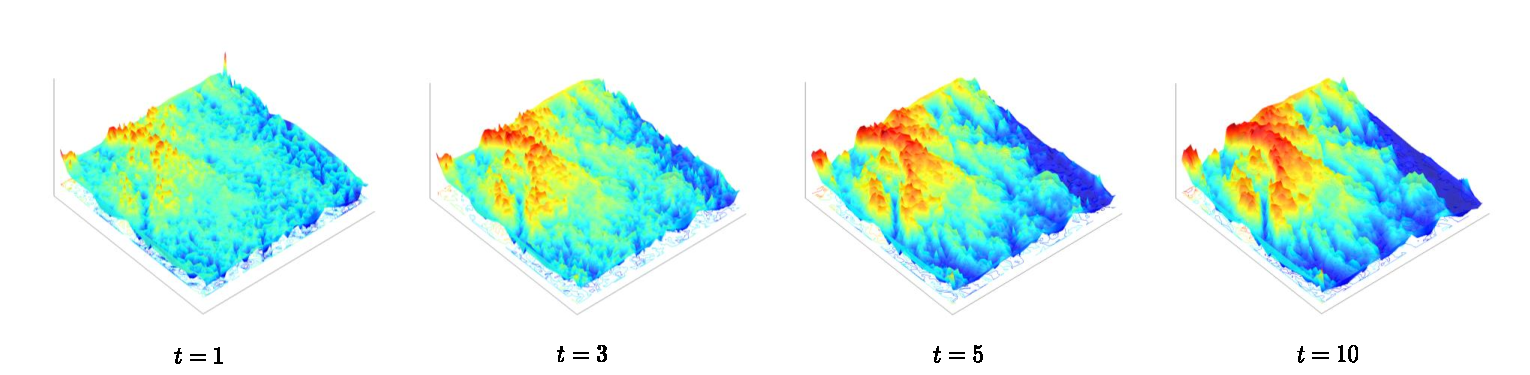
\includegraphics[width=6.5in]{figure/k_2_result}
%		\caption{$k=1$}
%	\end{subfigure}
%	\begin{subfigure}[b]{0.15\textwidth}
%		\centering
%		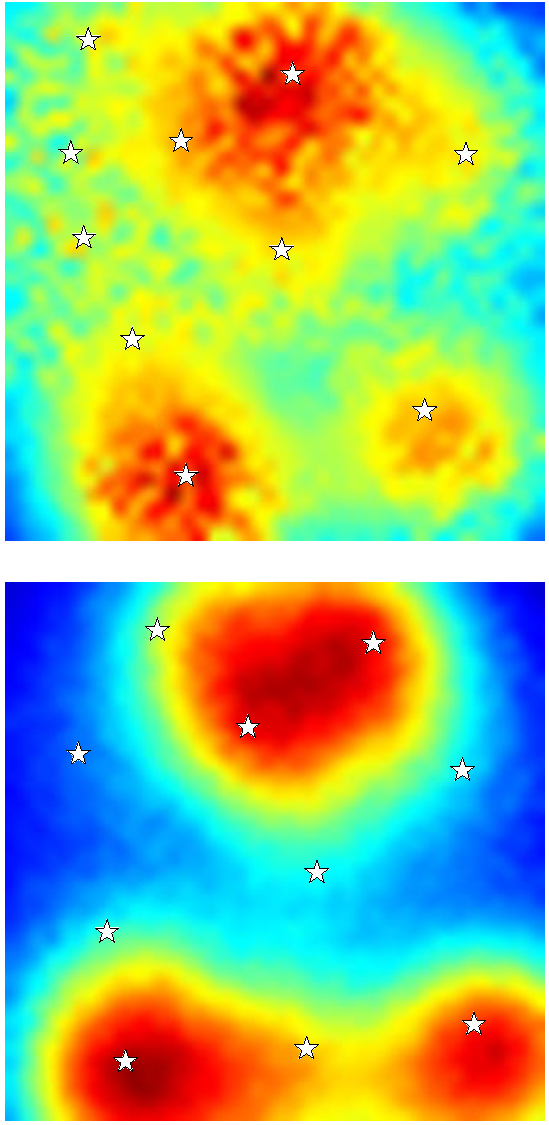
\includegraphics[width=1in]{figure/order2_step_0110_c}
%		\caption{$k=2$}
%	\end{subfigure}
%	 \begin{subfigure}[b]{0.15\textwidth}
%	\centering
%	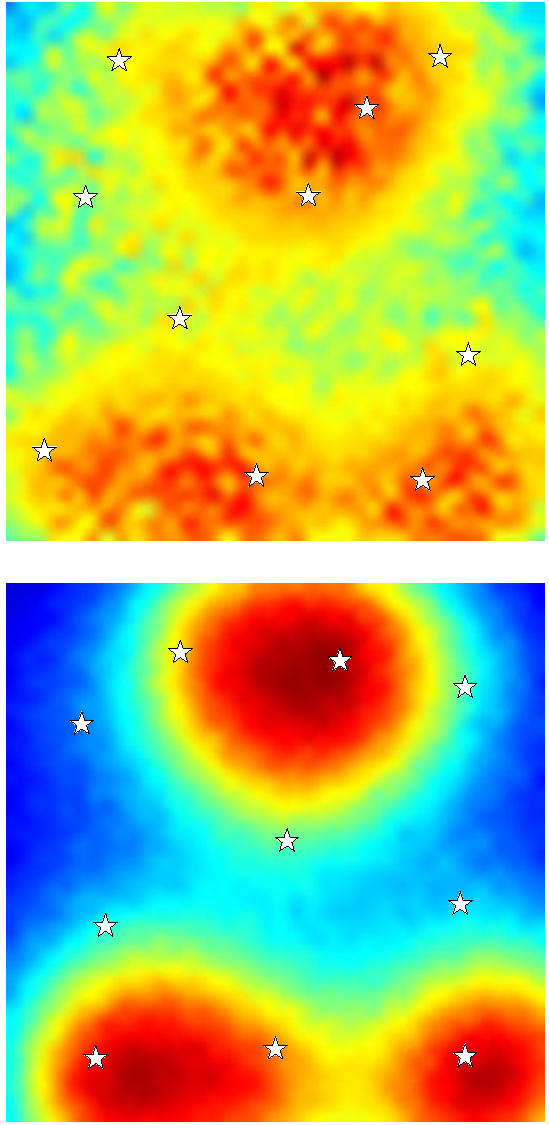
\includegraphics[width=1in]{figure/ordern_step_0110_c}
%	\caption{$k=10$}
%\end{subfigure}
	\caption{Time evolution of expected belief with robust method ($k=2$), $r_{\textup{eff}} = 2.89$, $\Sigma_B = 0.04\mathbf{I}$.}
	\label{fig:fig3}
\end{figure*}

\subsection{Convergence of our deployment algorithm}
First, the behavior of the deployment strategy is discussed. Given the initial uniform prior belief and the initial configuration at $x_0$, three algorithms, summarized in Table \ref{table2}, were tested.
Fig. \ref{fig:fig2} shows the configurations after $t=1$ with non-robust method (left) and robust method (right) where $k=2$. 
Fig. \ref{fig:fig0} compares the convergence speed and the cost between three methods.

\subsection{Environmental mapping/filtering performance w/o failure}
Next, we present the evolution of the object map given the uniform, initial map (Fig. \ref{fig:fig1}) with successive positive observations, each followed by the gradient descent strategy and filtering process. Fig. \ref{fig:fig3} illustrates the map building process, given limited effective sensing range value ($r_{\textup{eff}}=0.3$, the value was chosen empirically relative to the workspace size) when using our robust method. Others show similar performance, and are omitted due to the lack of space.
%
%
%The results in Fig. \ref{fig:fig3} clearly show that under \emph{limited} sensing range, the non-coordinated strategy ($k=1$) yields relatively better mapping results than coordinated strategies ($k=2,\,10$) compared to the ground truth map shown in Fig \ref{fig:fig1}.
Fig. \ref{fig:fig5} compares the K-L divergence values between different strategies during the evolution. While the max. information gain approach shows the best result, other methods also shows competitive mapping performance compared to the ground truth.
%The occurrence of sudden jumps (between the time step 0 and 1) in the K-L divergence values observed in Fig \ref{fig:fig5}(a) demonstrates the cases when the initial uniform density happened to a better `\emph{guess}' than the crude belief obtained after a single propagation of the filtering process.
\begin{figure}
	\centering
	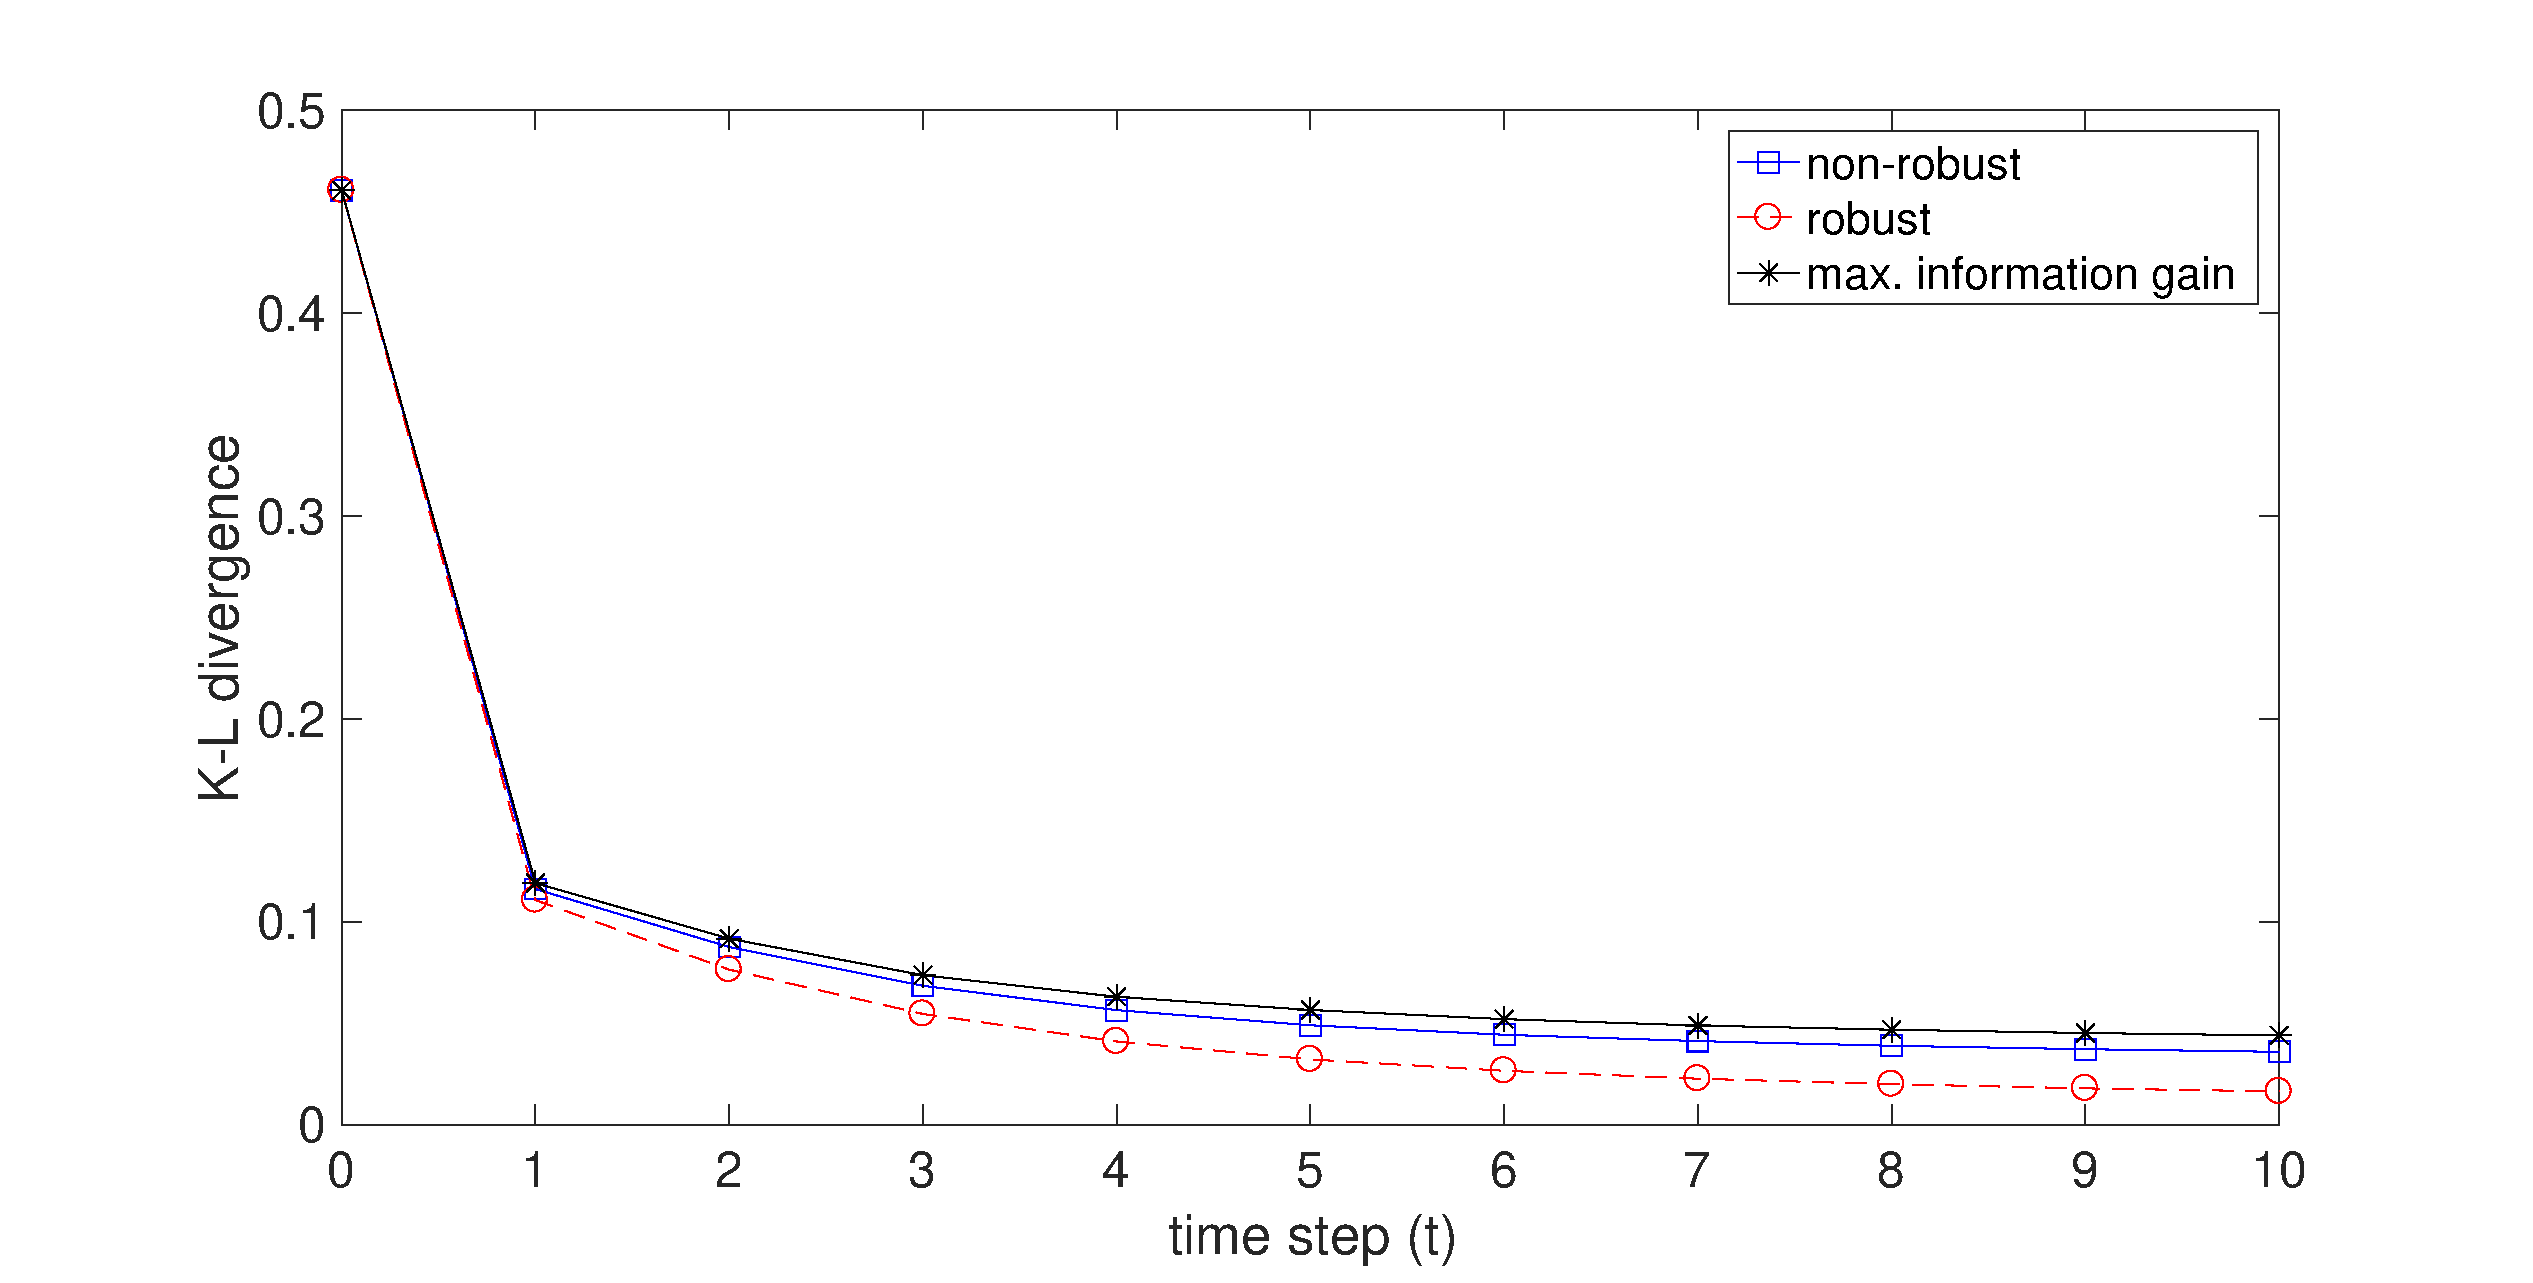
\includegraphics[width=2.9in]{figure/cost_comp0}
	\caption{Comparison of K-L divergence from the actual distribution between different methods during belief propagation.}
	\label{fig:fig5}
\end{figure}
%\begin{figure}
%	\centering
%	\begin{subfigure}[b]{0.15\textwidth}
%		\centering
%		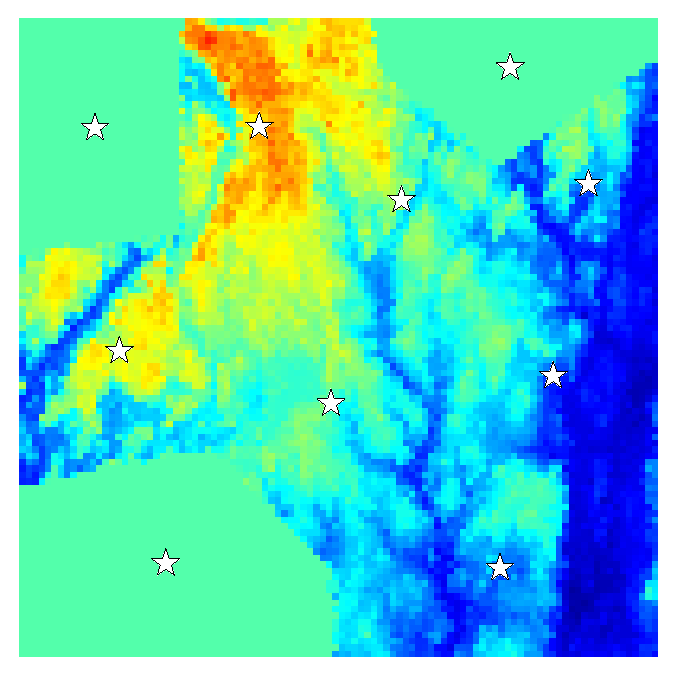
\includegraphics[width=1in]{figure/k_1}
%		\caption{$k=1$}
%	\end{subfigure}
%	\begin{subfigure}[b]{0.15\textwidth}
%		\centering
%		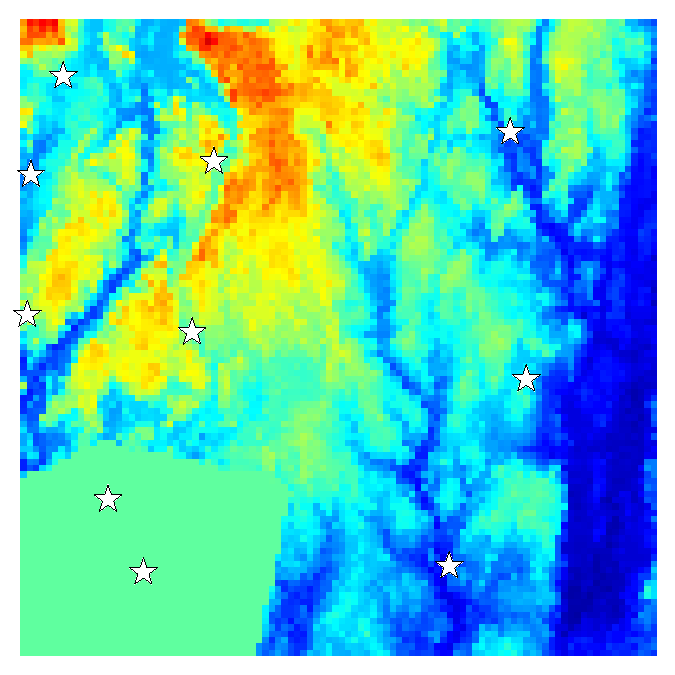
\includegraphics[width=1in]{figure/k_2}
%		\caption{$k=2$}
%	\end{subfigure}
%	\begin{subfigure}[b]{0.15\textwidth}
%	\centering
%	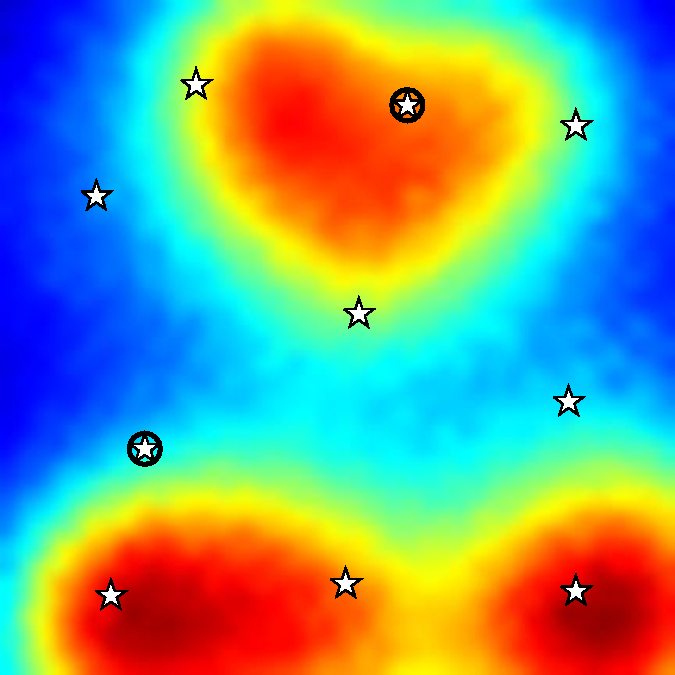
\includegraphics[width=1in]{figure/fault_order_n_c}
%	\caption{$k=10$}
%\end{subfigure}
%	\caption{Comparison of robots' configuration and beliefs at the final step with two approaches, $k=1, \,2,\,10$ when two of the sensors fails (circled) and $r_{\textup{eff}}=\infty$, $\Sigma_B = 0.04\mathbf{I}$ for both cases }
%	\label{fig:fig6}
%\end{figure}
%\begin{figure}
%	\centering
%	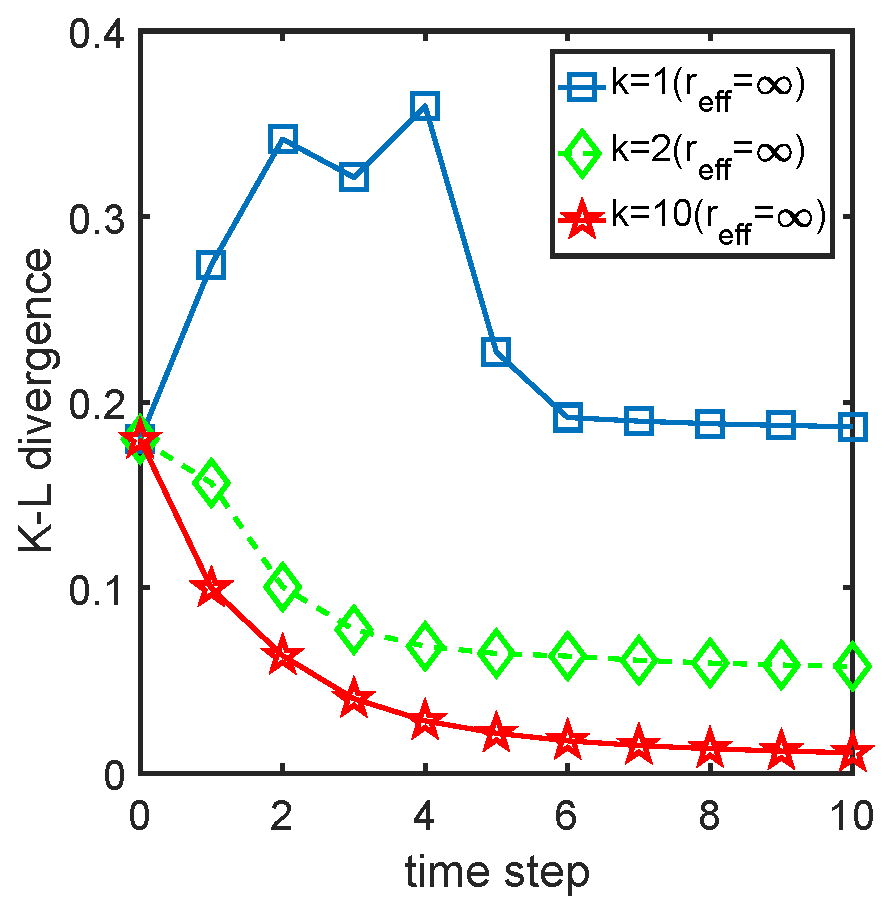
\includegraphics[width=1.6in]{figure/fault_kl2}
%	\caption{Comparison of K-L divergence of the ground-truth between multiple strategies ($k=1,\,2,\,10$), when two sensors fail during the evolution}
%	\label{fig:fig7}
%\end{figure}

\subsection{Robustness to sensor failure}
This section will present a number of examples when robust method become more appealing than non-robust method, which happens when the sensors are prone to fail. 
We consider three different cases, when $\mathcal{F} = \lbrace 1 \rbrace,\,\lbrace 1,2\rbrace,\,\lbrace 1,2,3 \rbrace$.
Results for robots configuration and target distributions after $10^{\textup{th}}$ step with non-robust and robust methods in the case when $\mathcal{F}= \lbrace 1\rbrace$ are shown in Fig. \ref{fig:fig6}. 
As can be seen from Fig \ref{fig:fig6} and Fig. \ref{fig:fig7}, the map retrieved by the proposed method $k=2$ is more robust to the sensor failure compared to that obtained with the non-robust method. In Fig \ref{fig:fig6}, both middle and right, the unmapped area is owe to the limited sensing range.
It is not surprising to see from this example that the maximum information gain method shows the best robustness to sensor failures among the three; however this is due to the help from the central information fusion sever and relatively large communication load.
\begin{figure}
	\centering
	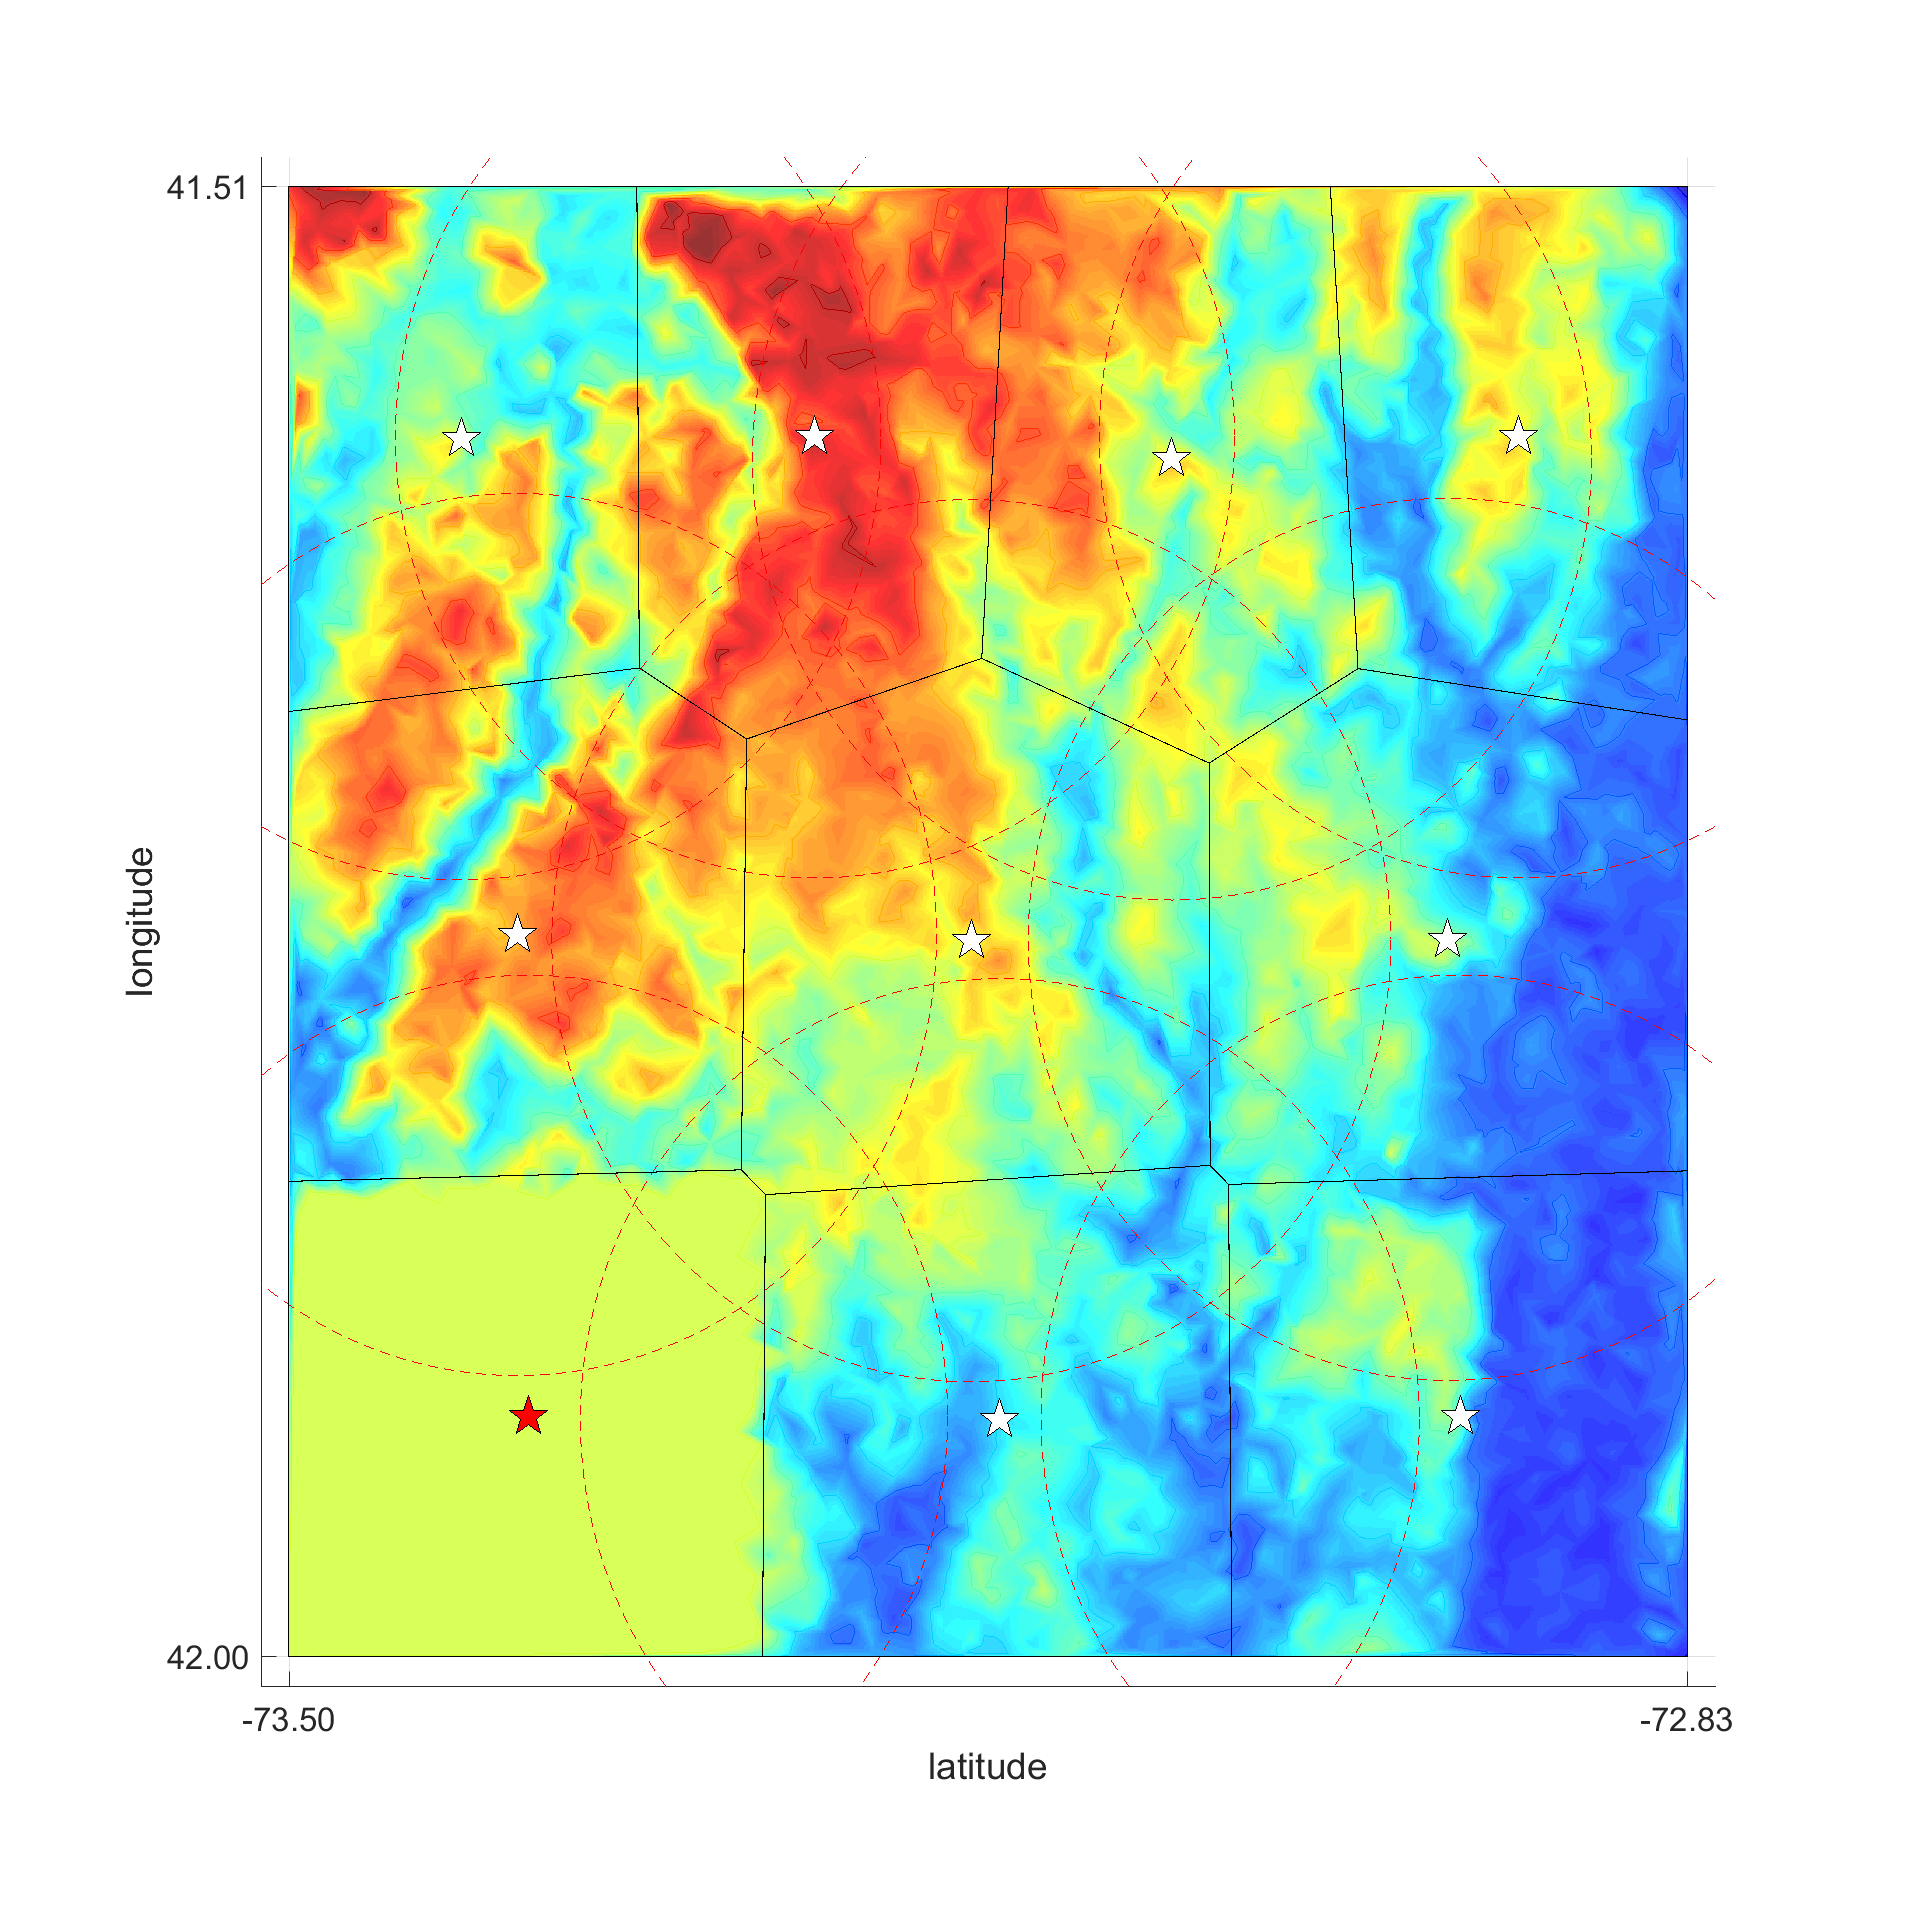
\includegraphics[width=1.1in]{figure/order1_conf}
	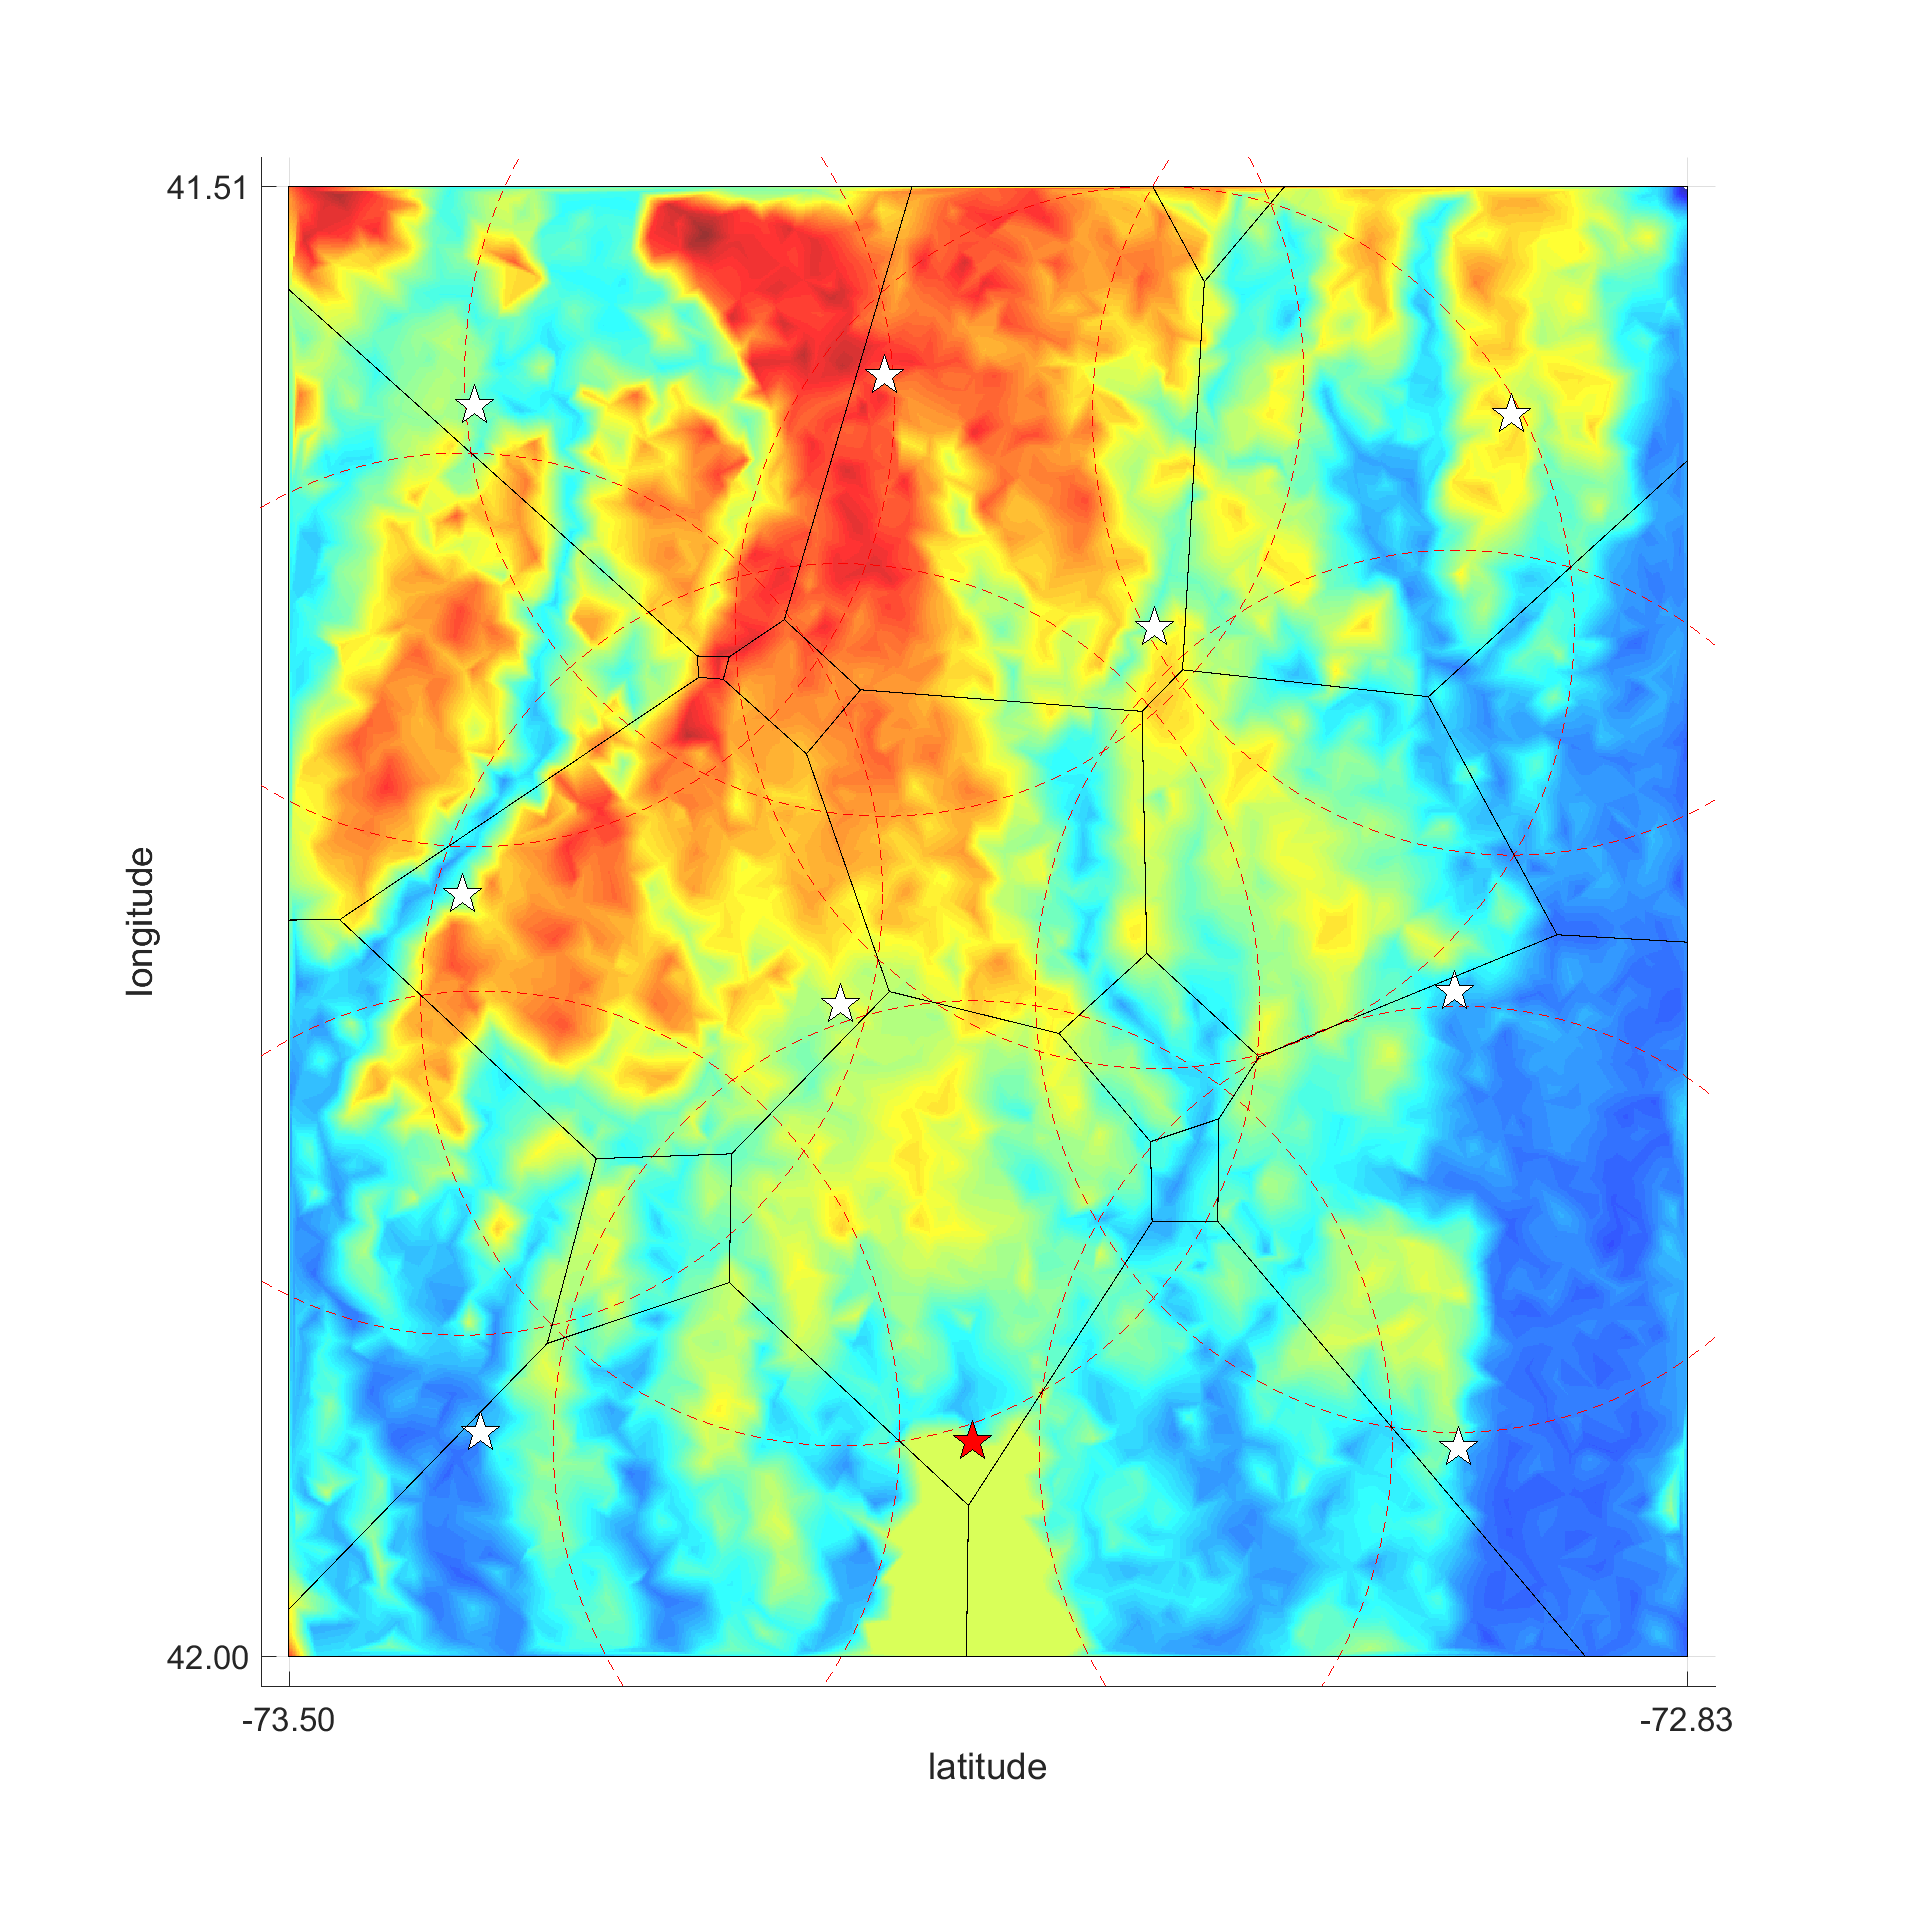
\includegraphics[width=1.1in]{figure/order2_conf}
	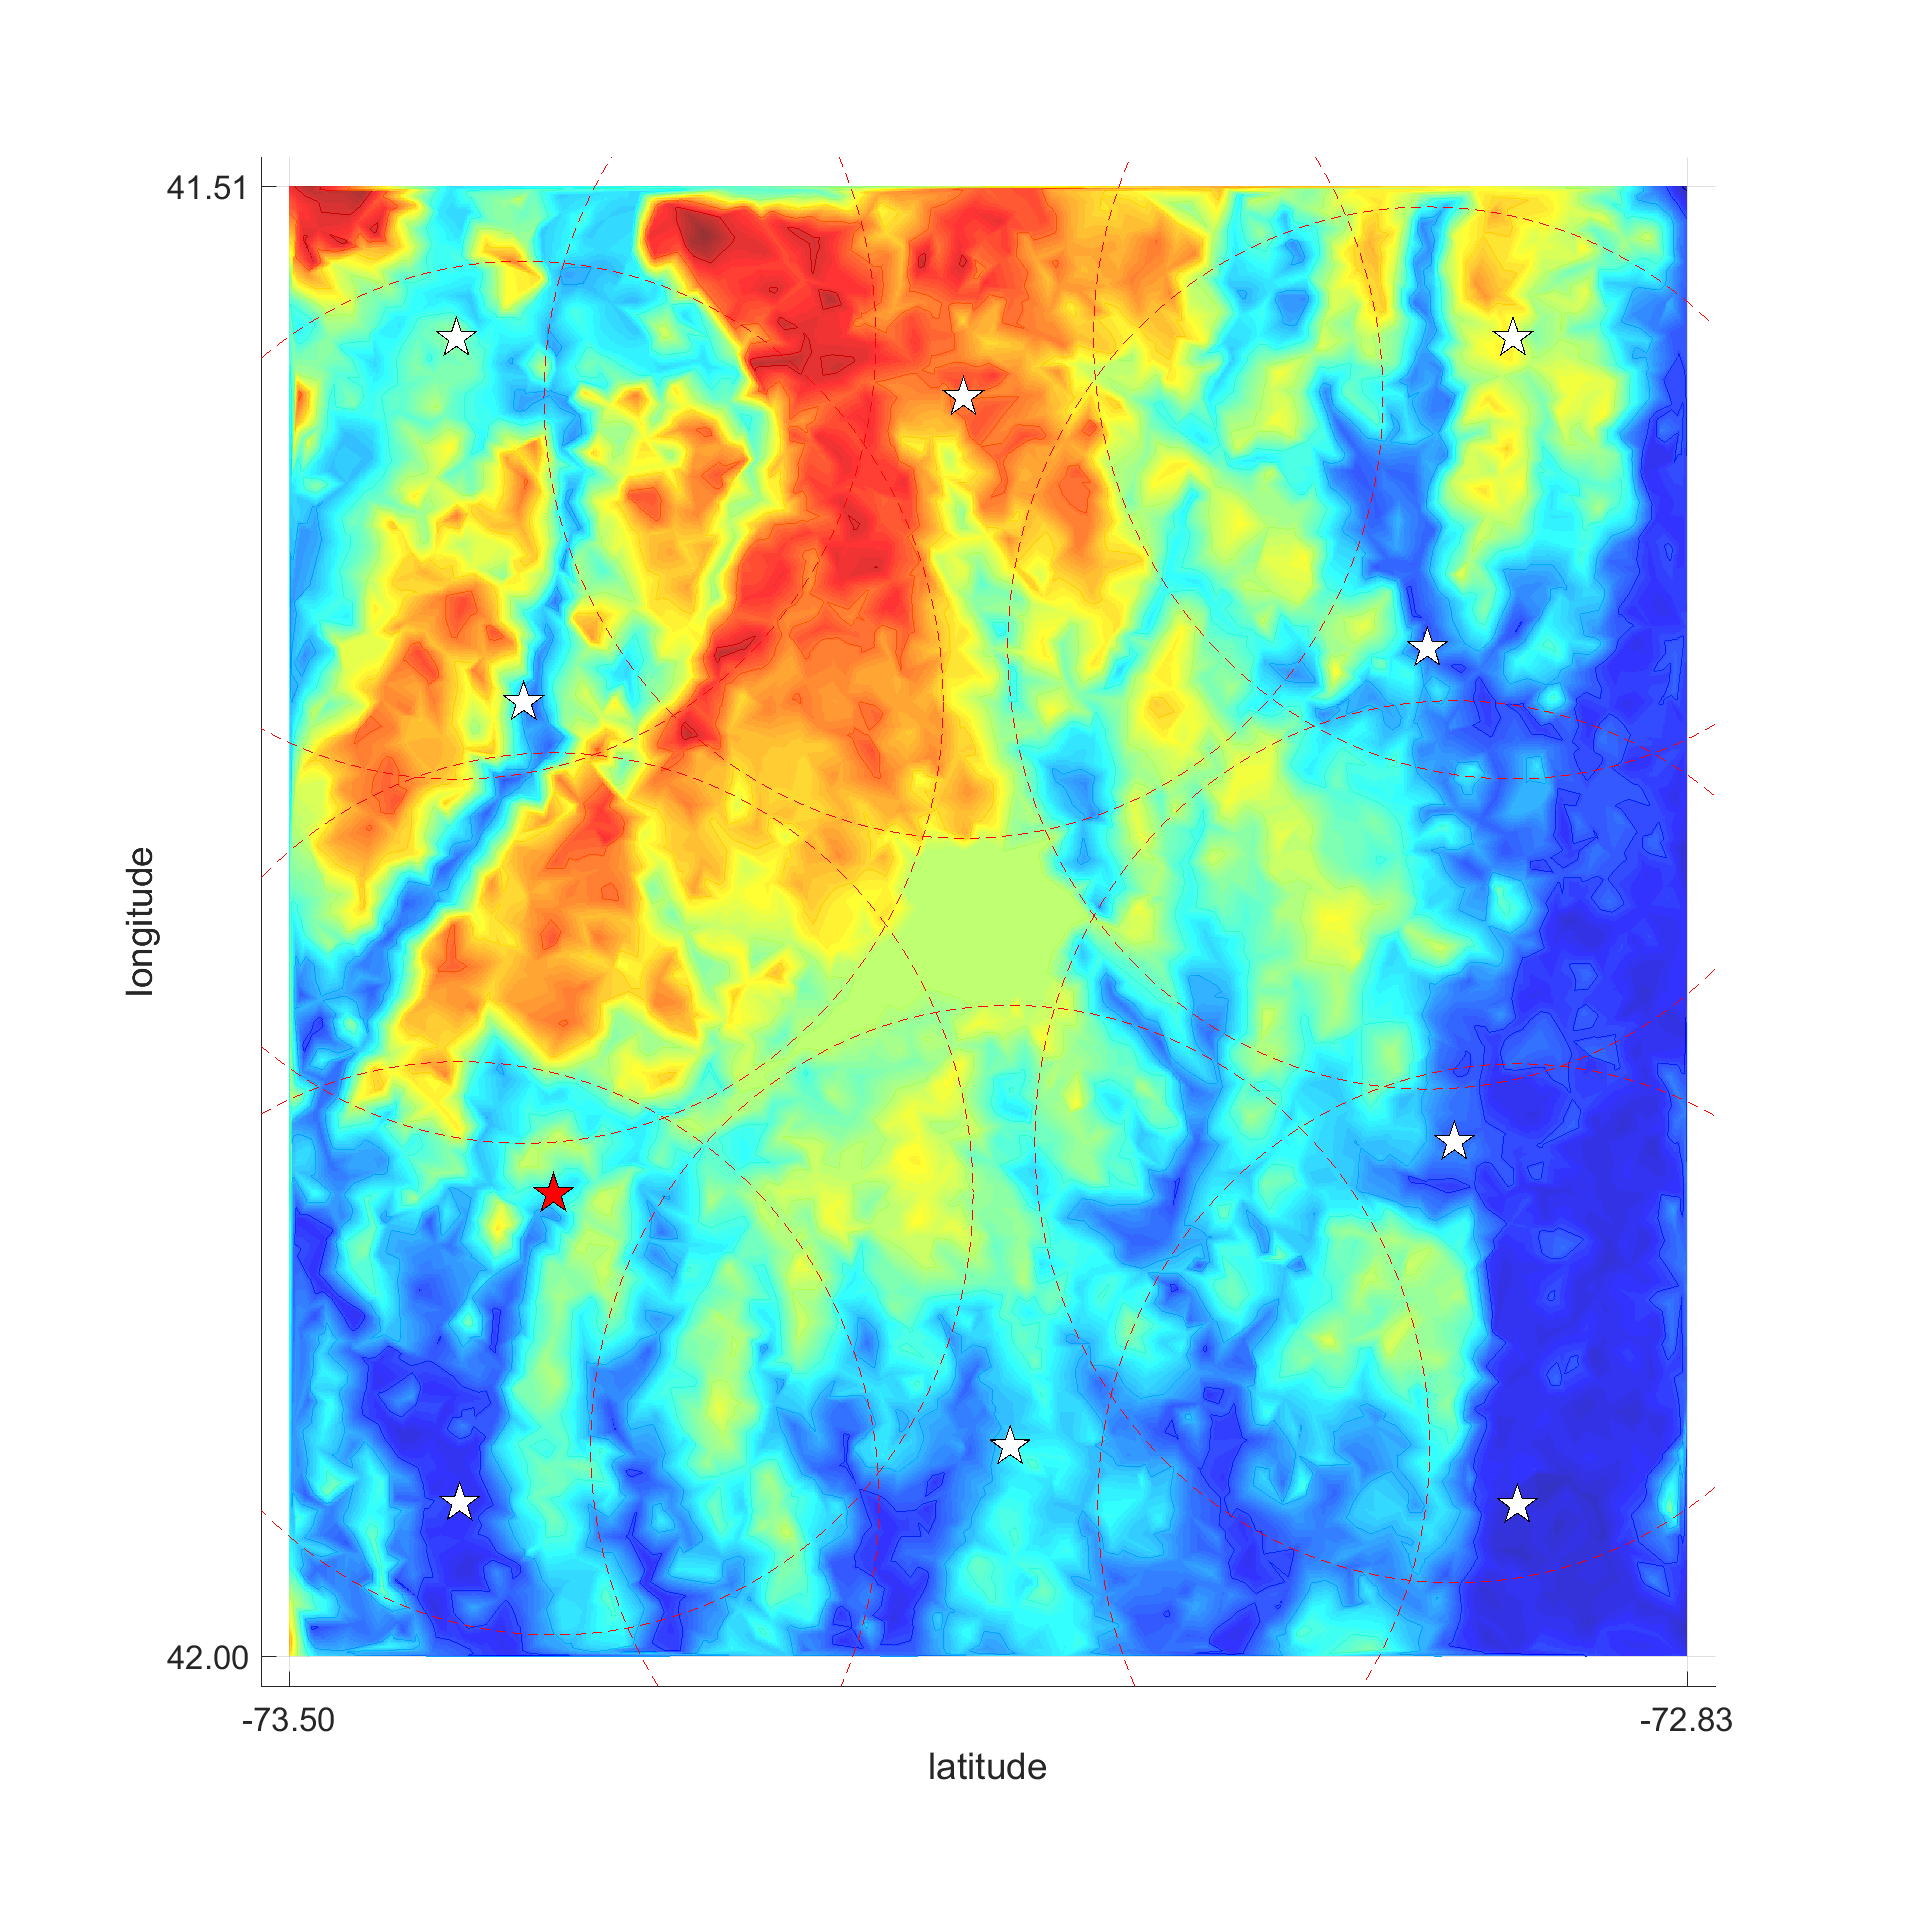
\includegraphics[width=1.1in]{figure/final_config_ordern_fault}
	%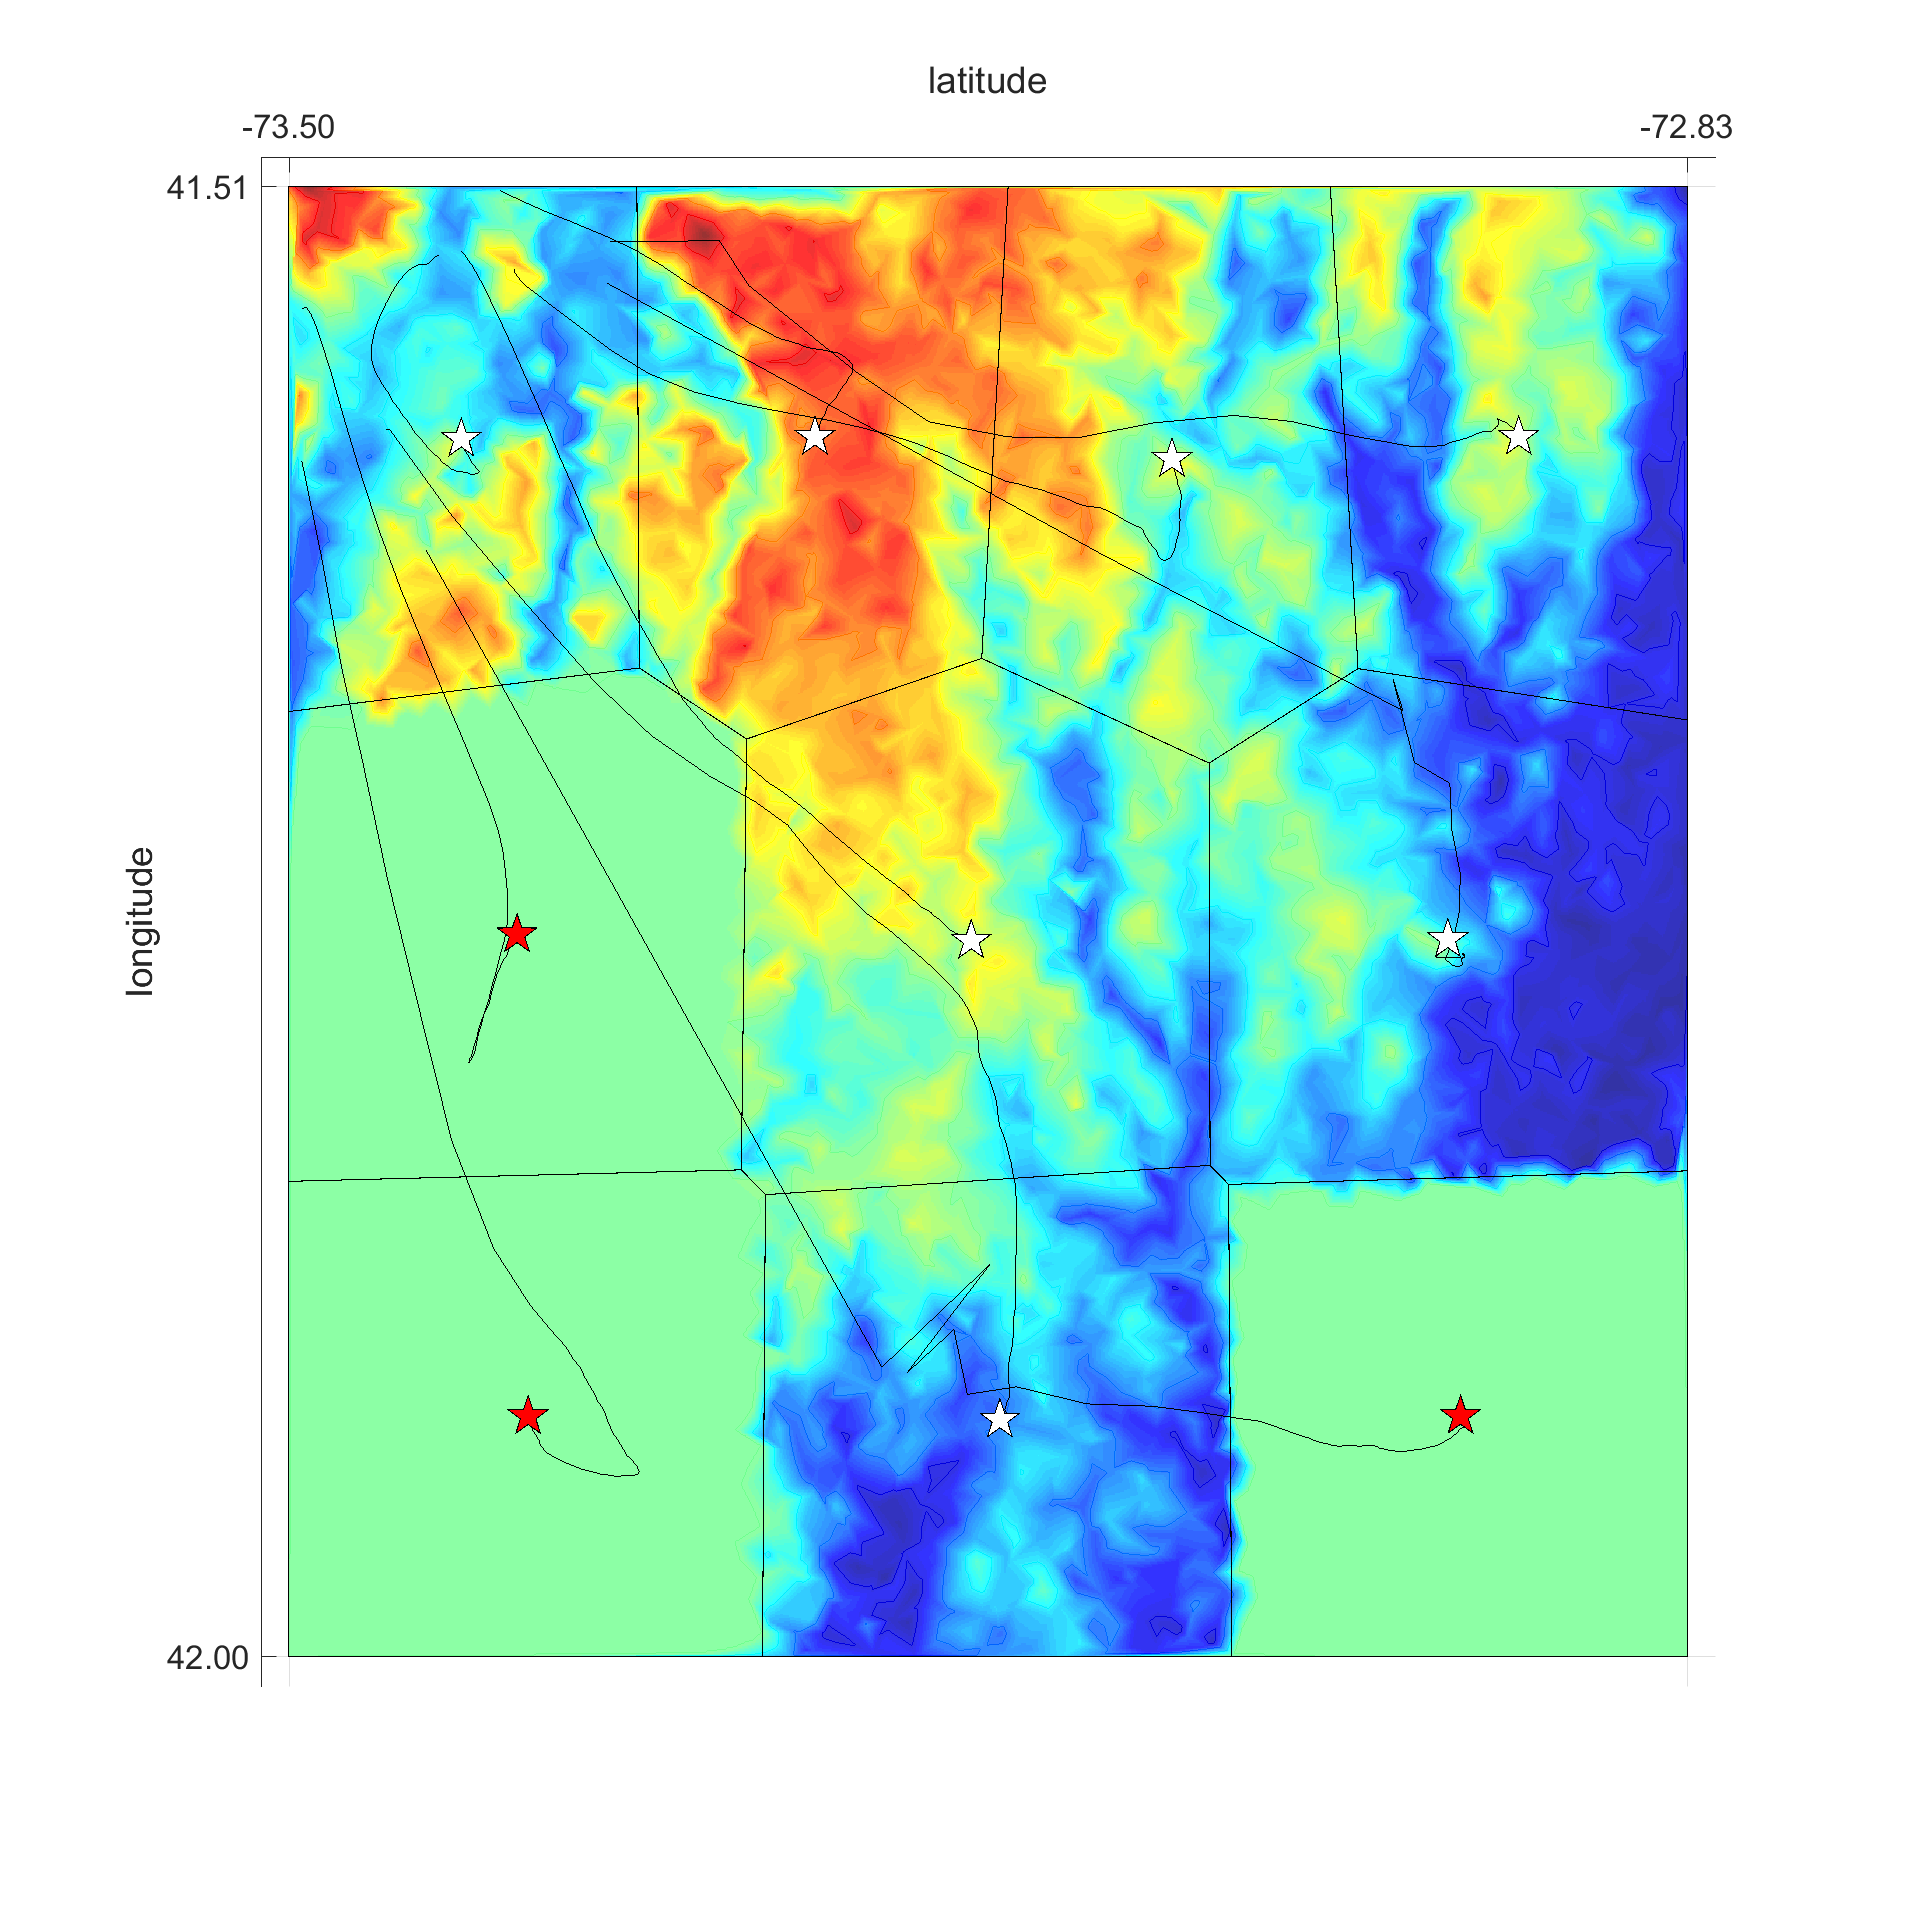
\includegraphics[width=1.57in]{figure/final_config_order1_fault}
	%	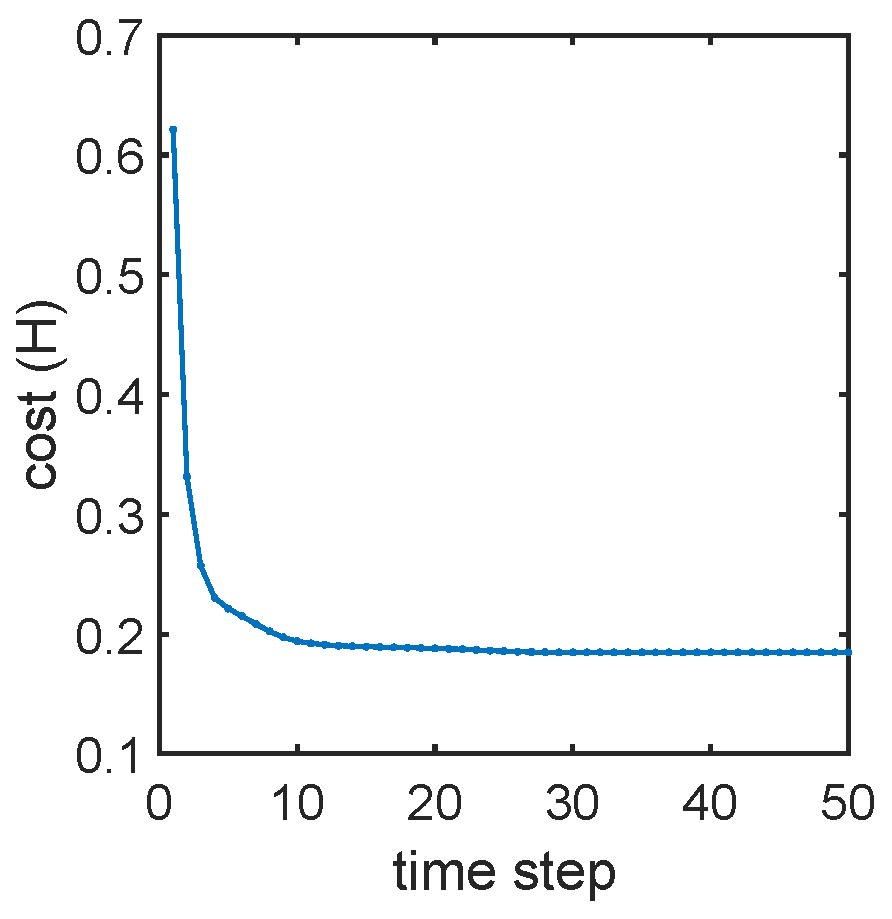
\includegraphics[width=3.4in]{figure/init_10_deploy_cmd2}
	\caption{The belief at $t=10$ with non-robust method (left) and robust method (middle), and max. information method (right) Also showing robot configurations (stars, where red stars are robots whose sensors have failed), effective sensing range (dashed line), and partition (solid lines).
	}
	\label{fig:fig6}
\end{figure}
\begin{figure}
	\centering
	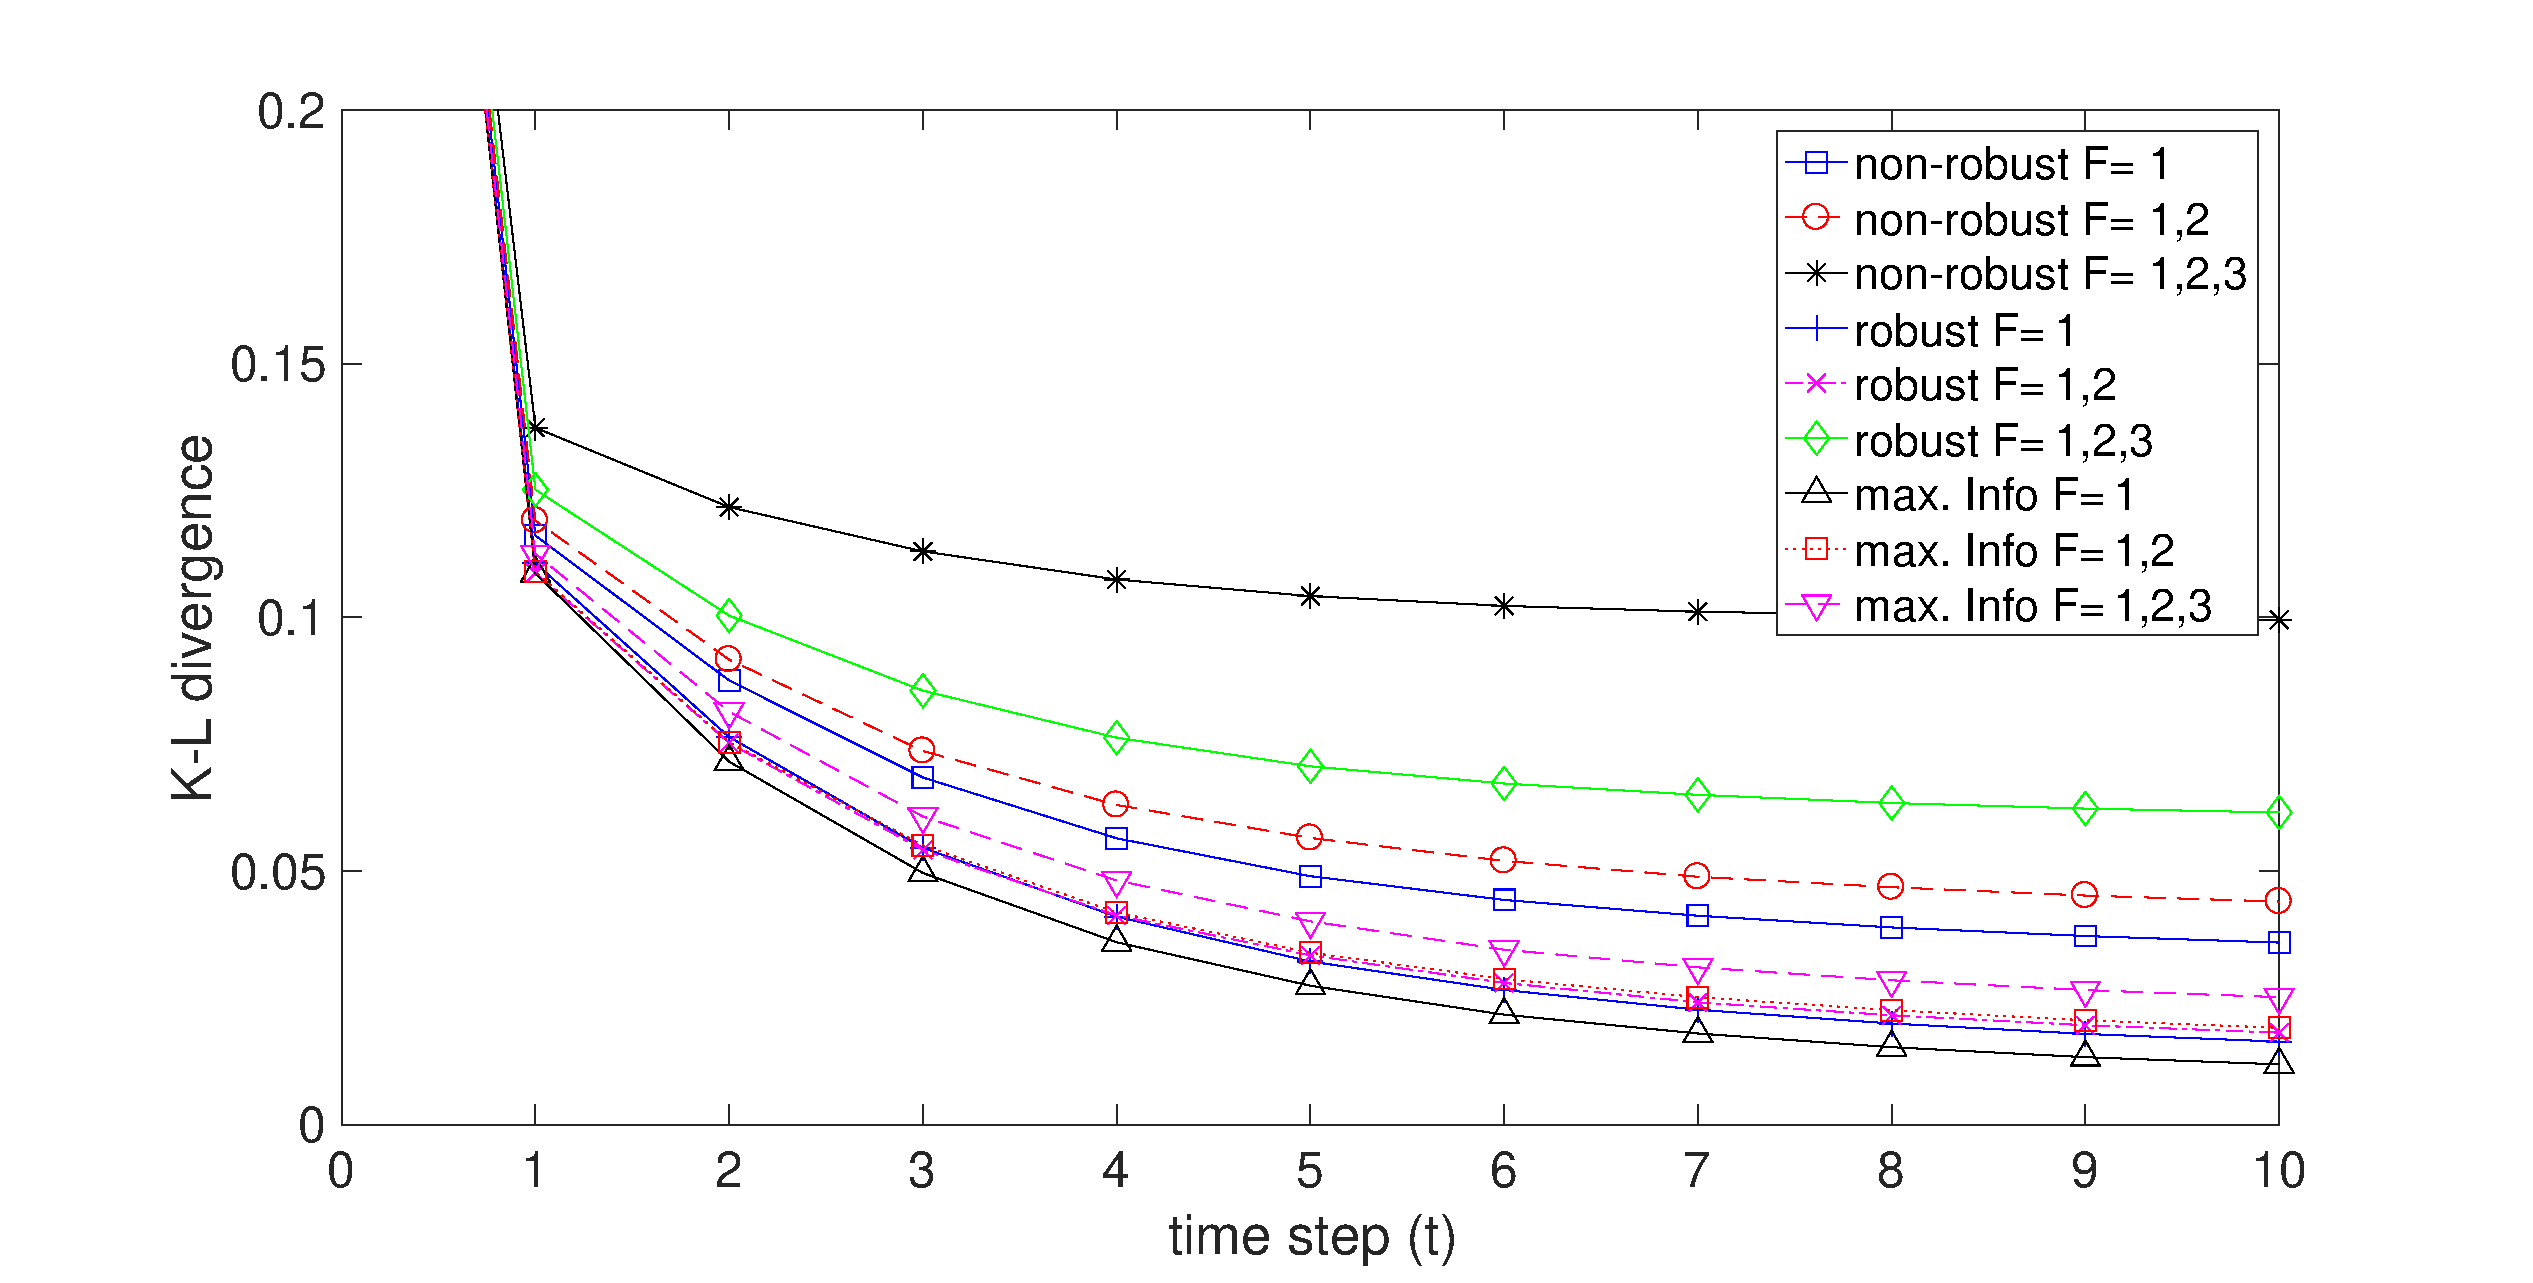
\includegraphics[width=2.9in]{figure/cost_comp000}
	\caption{Comparison of K-L divergence from the actual distribution between different methods during belief propagation when part of the sensor fail.}
	\label{fig:fig7}
\end{figure}


\subsection{Statistical results with different initial conditions/faults compositions}
Statistical results shows that our method can be used to estimate arbitrary target distribution given randomly chosen initial configuration, with different fault compositions reasonably well. 
Fig. \ref{fig:fig8} shows a distribution of K-L divergence values at the $t=10$ for a given $100$ random initial configurations with randomly sampled faults $1\leq \left|\mathcal{F}\right| \leq 5$.
\begin{figure}
	\centering
	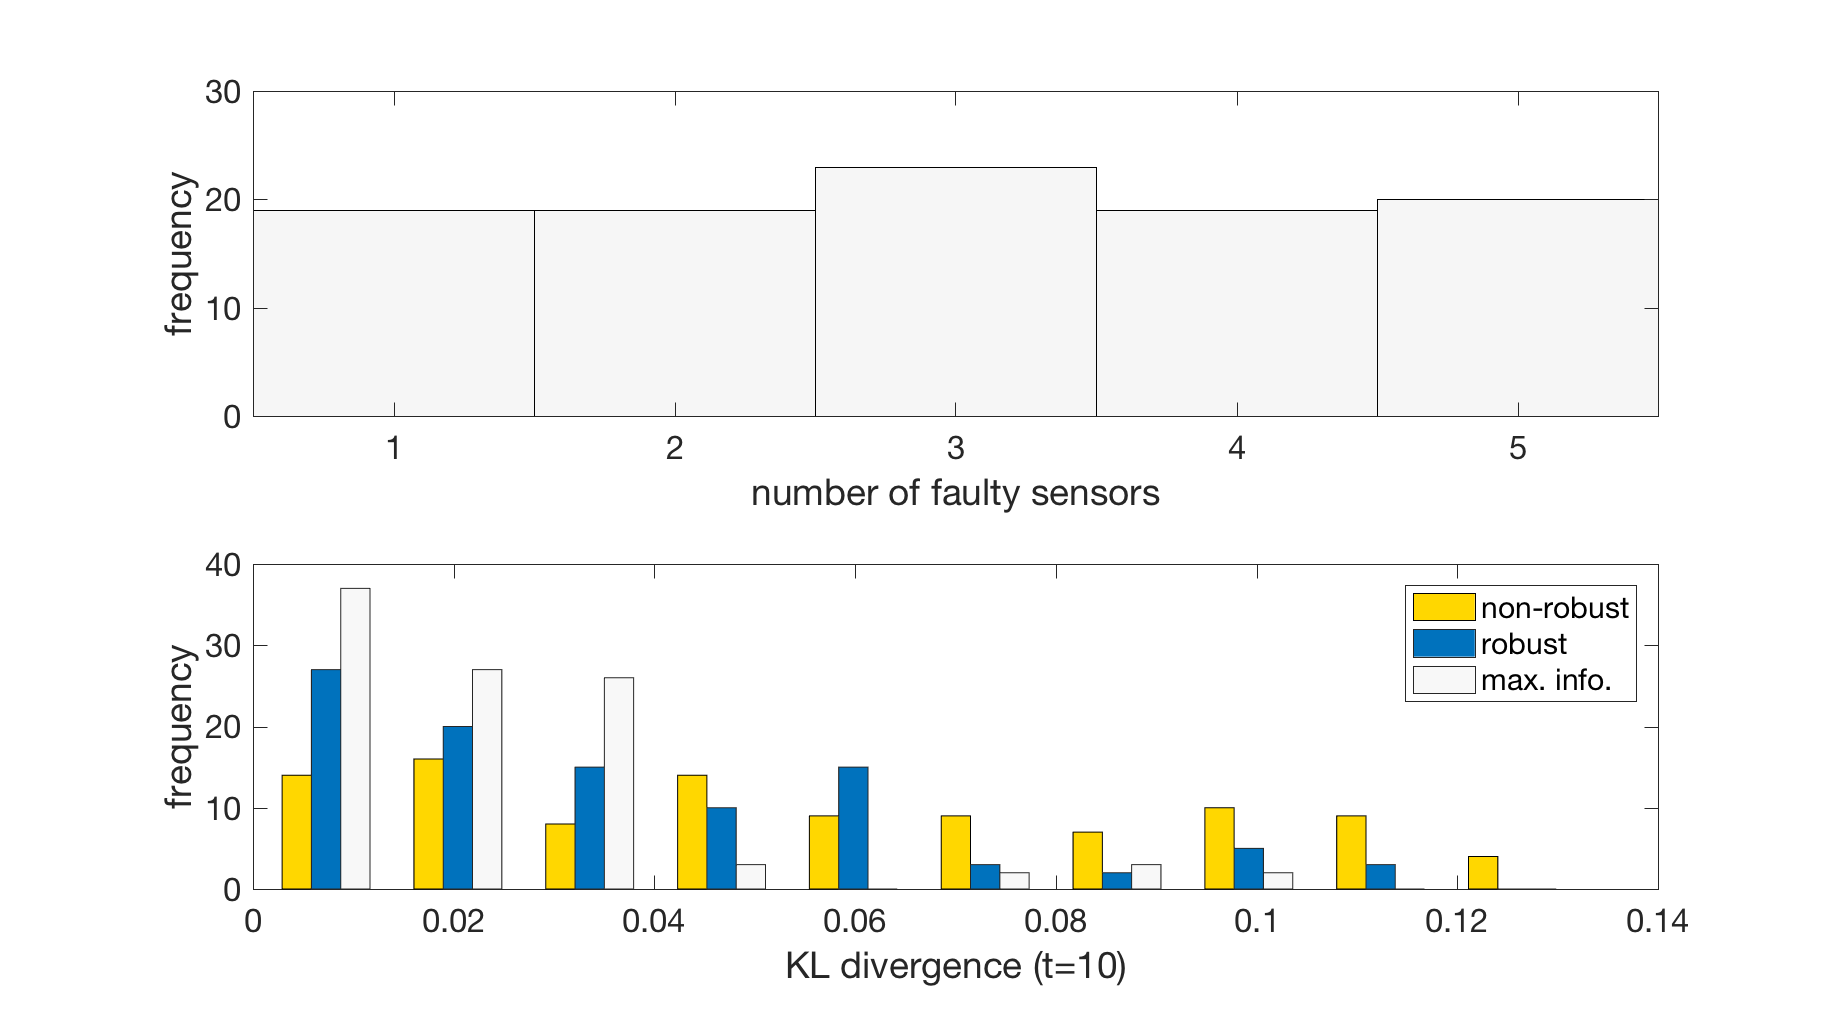
\includegraphics[width=2.7in]{figure/stat_result}
	\caption{Robustness test with 100 test dataset, distribution of $\left|\mathcal{F}\right|$ (top), K-L divergence at $t=10$ (bottom).} 
	\label{fig:fig8}
\end{figure}

%\begin{table}[]
%	\centering
%	\caption{Mean and standard deviations (parenthesis) of K-L divergence for  arbitrary distributions under 100 random initial configurations with fault compositions [WILL REPLACE THIS WITH HISTOGRAM...]}
%	\label{table1}
%			{\scriptsize
%	\resizebox{\linewidth}{!}{%	
%	\begin{tabular}{llllll}
%		\hline
%		Distribution type:           & \#1 & \#2 & \#3 & \#4 & \#5 \\ \hline
%		\multirow{2}{*}{K-L divergence} &  0.0358   &  0.0308   & 0.0495    &  0.0293   &  0.0339   \\ 
%	& (0.0034)    &  (0.0033)   &   (0.0041)  &  (0.0012)   &  	(0.0024)   \\ \cline{1-6}
%	\end{tabular}}}
%\end{table}



\subsection{Scalability of our method}
We also conducted a series of simulations and have validated that the previous results generalize to larger number of robots
Fig. \ref{fig:fig0} shows one of the results with $50$ robots after $t-10$ where robots' sensing ranges (dashed lines) and the order-$2$ Voronoi partition (solid lines) are overlaid over the expected belief.
\begin{figure}
	\centering
%	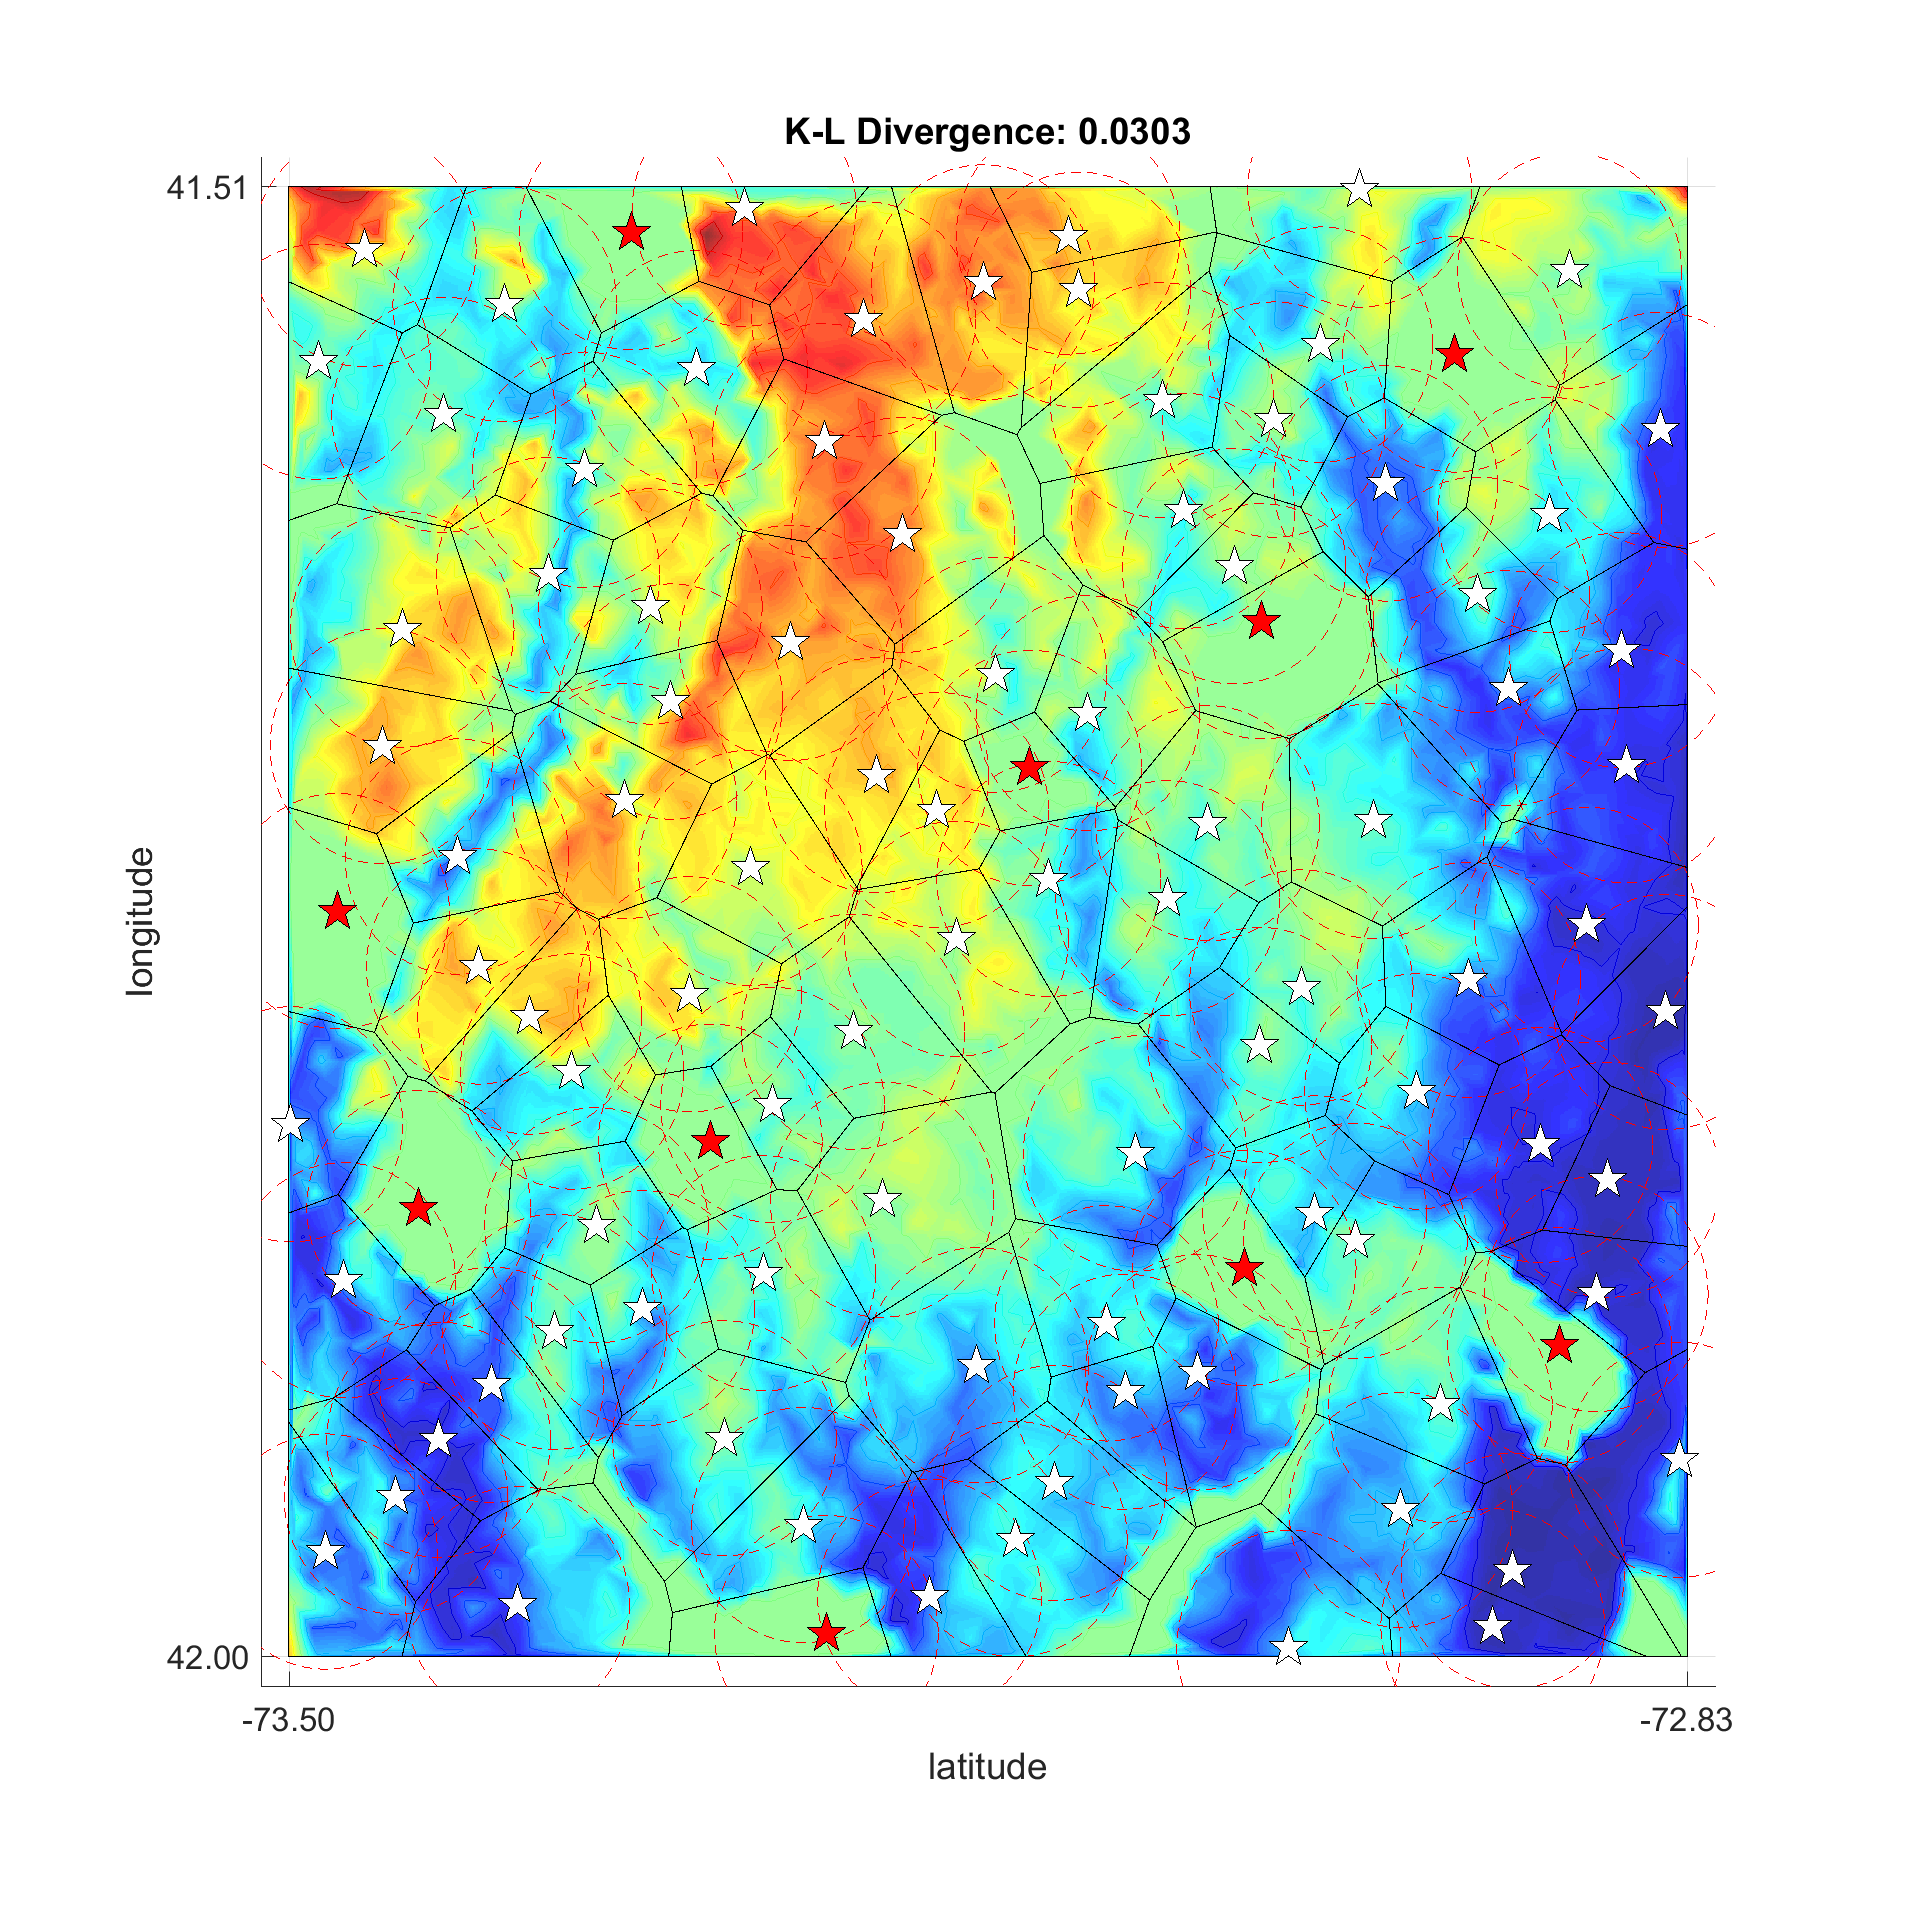
\includegraphics[width=1.1in]{figure/100_order1}
	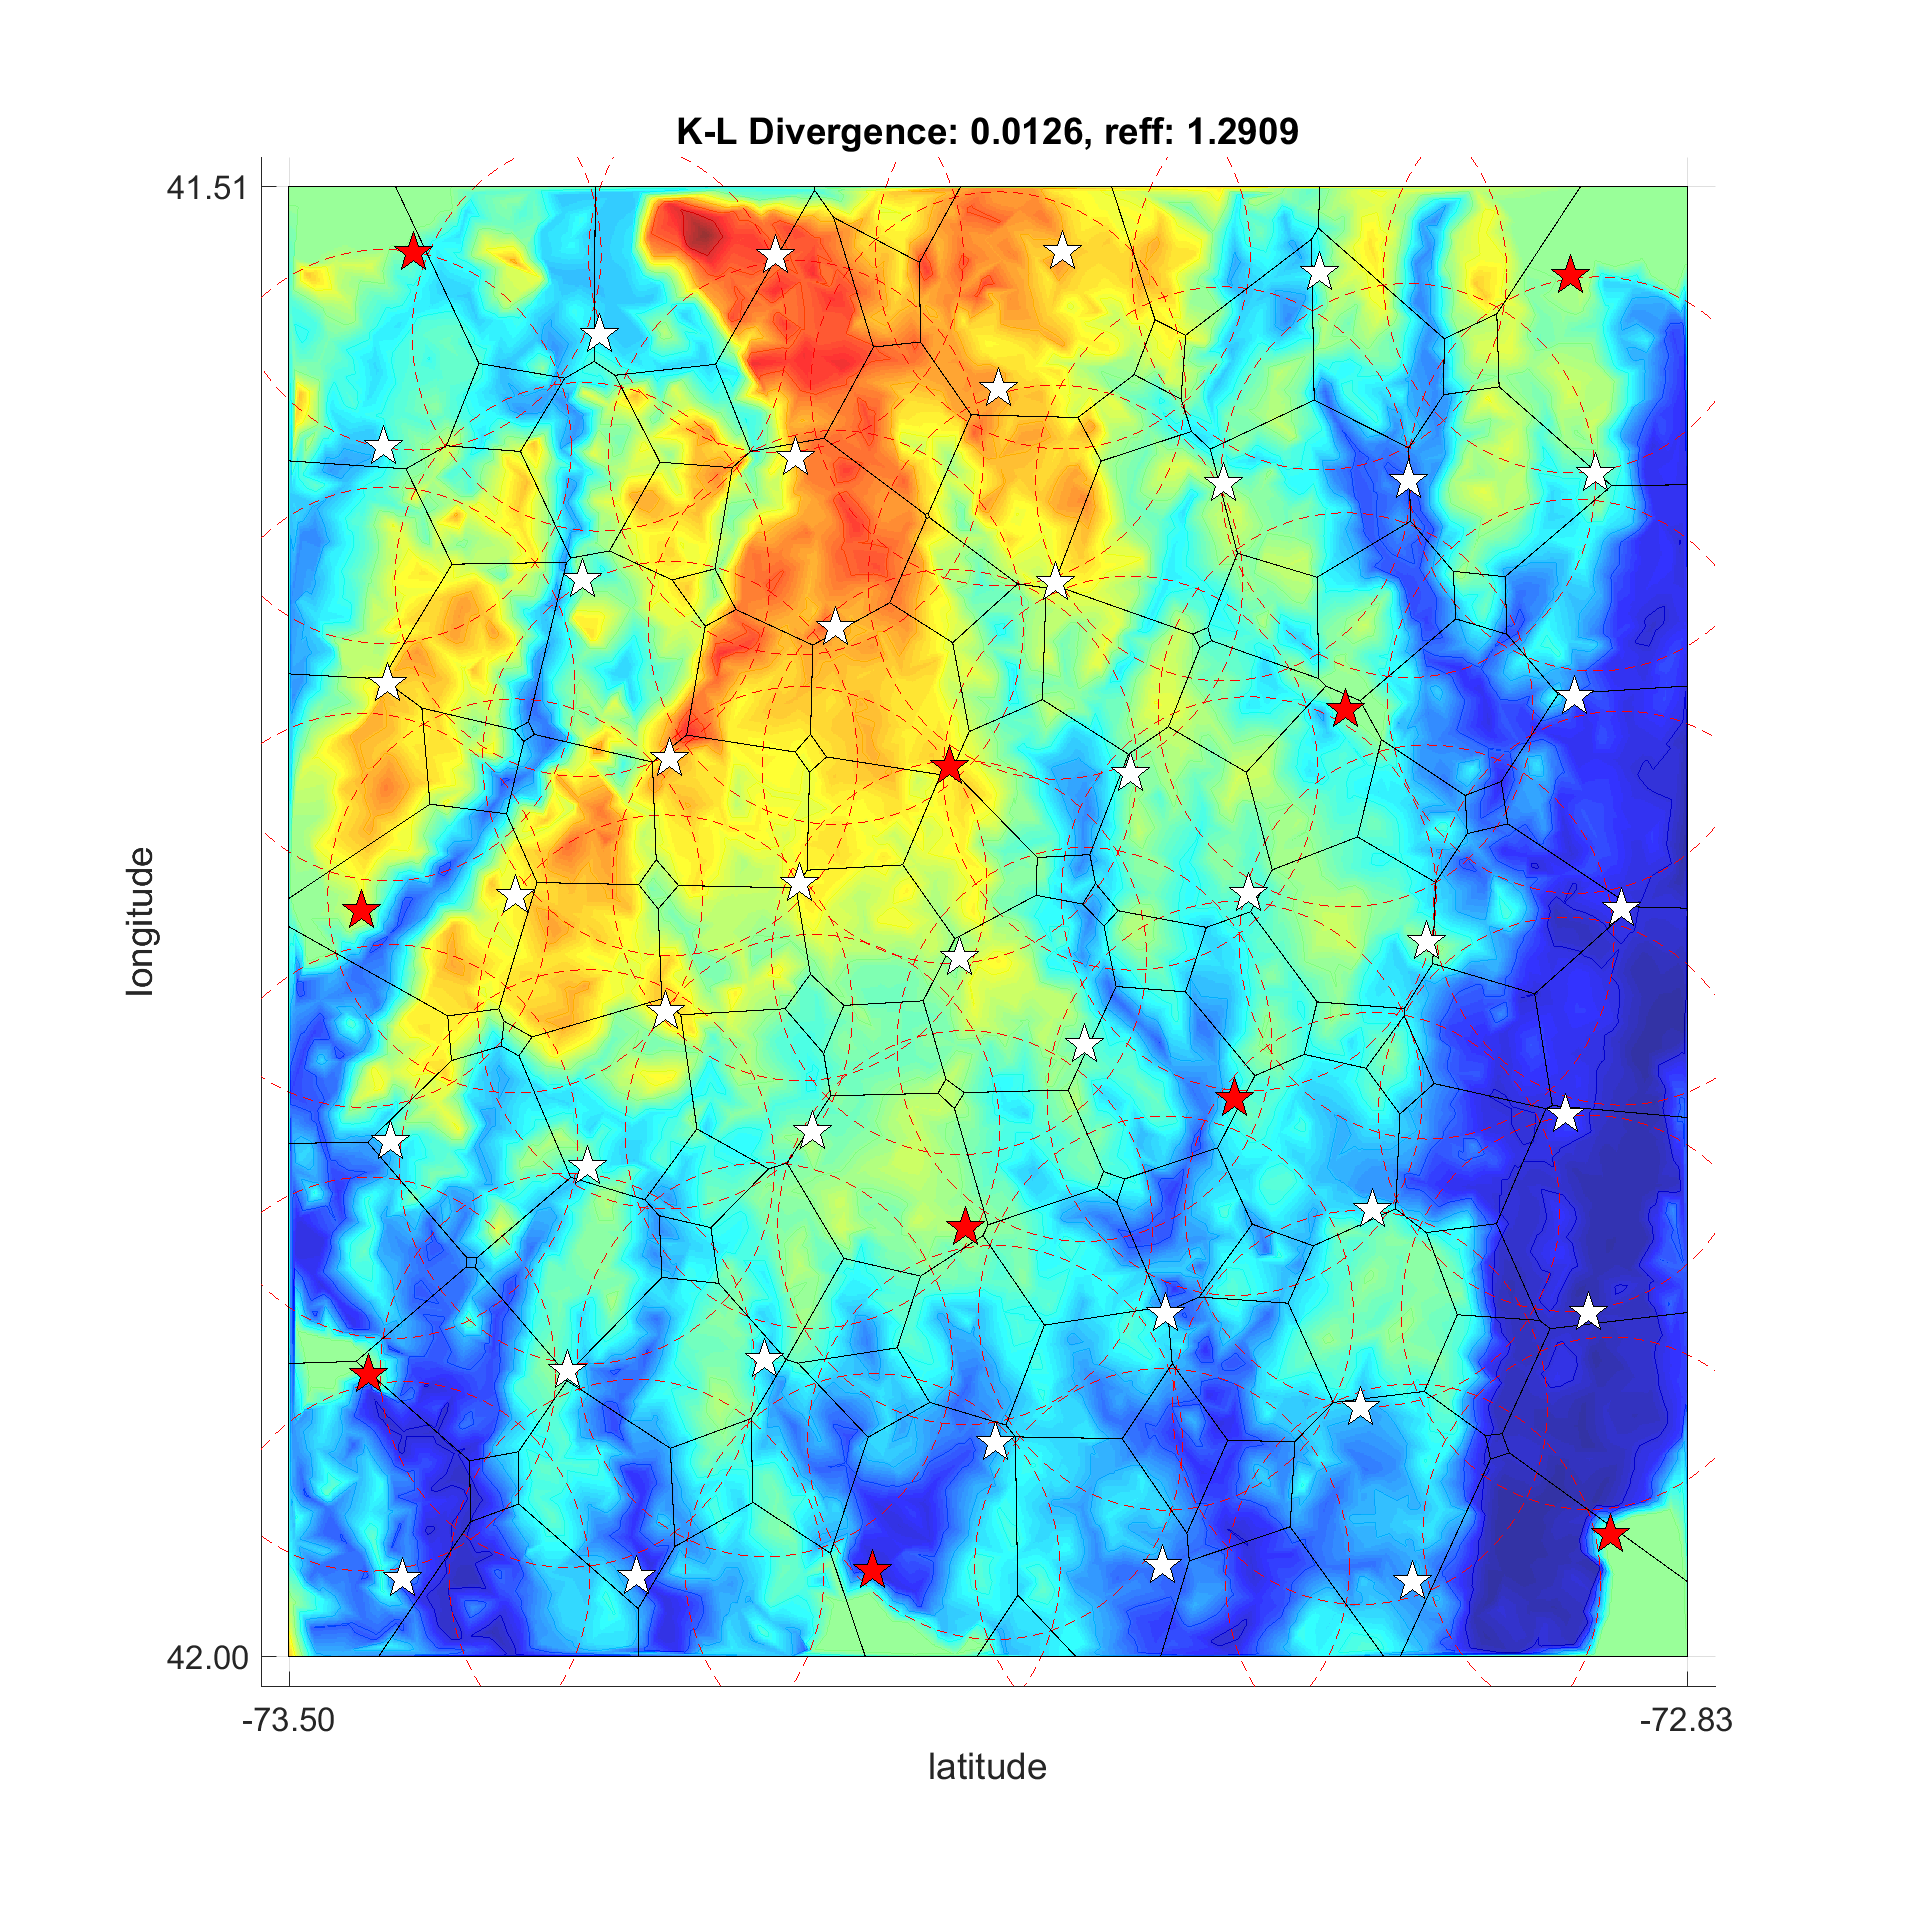
\includegraphics[width=2.7in]{figure/50_order2_last}
%	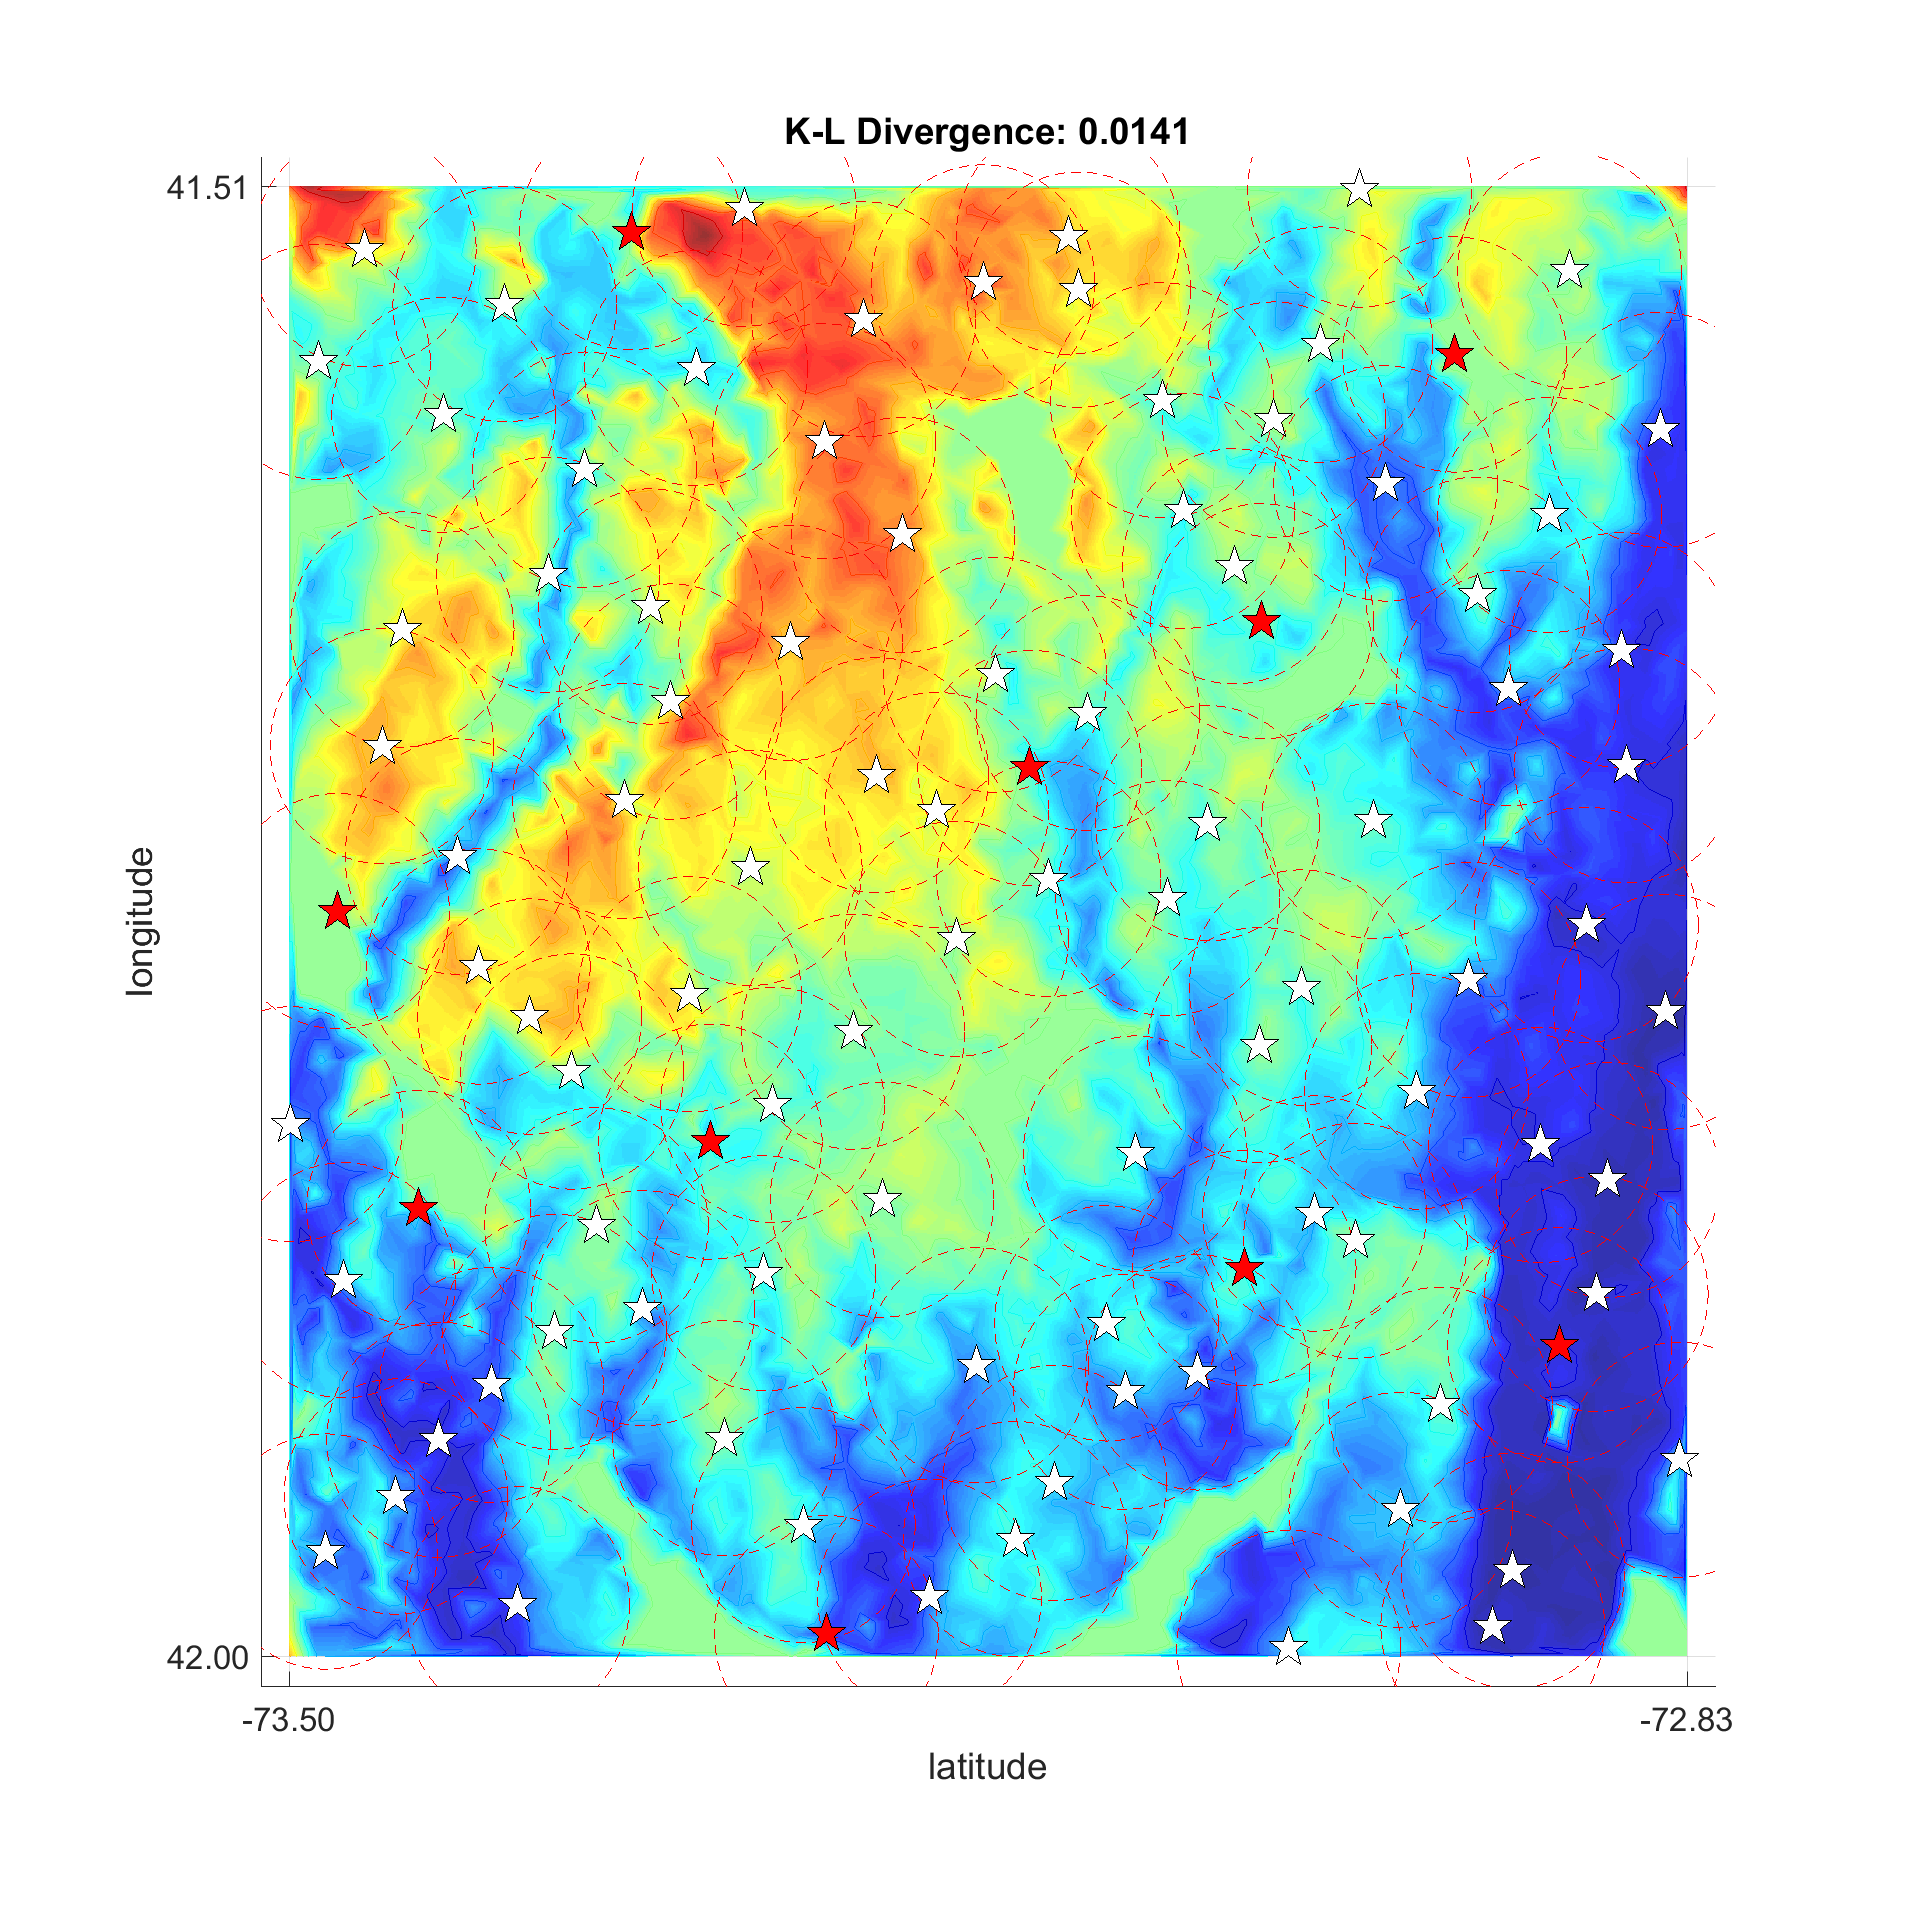
\includegraphics[width=1.1in]{figure/100_ordern}
	%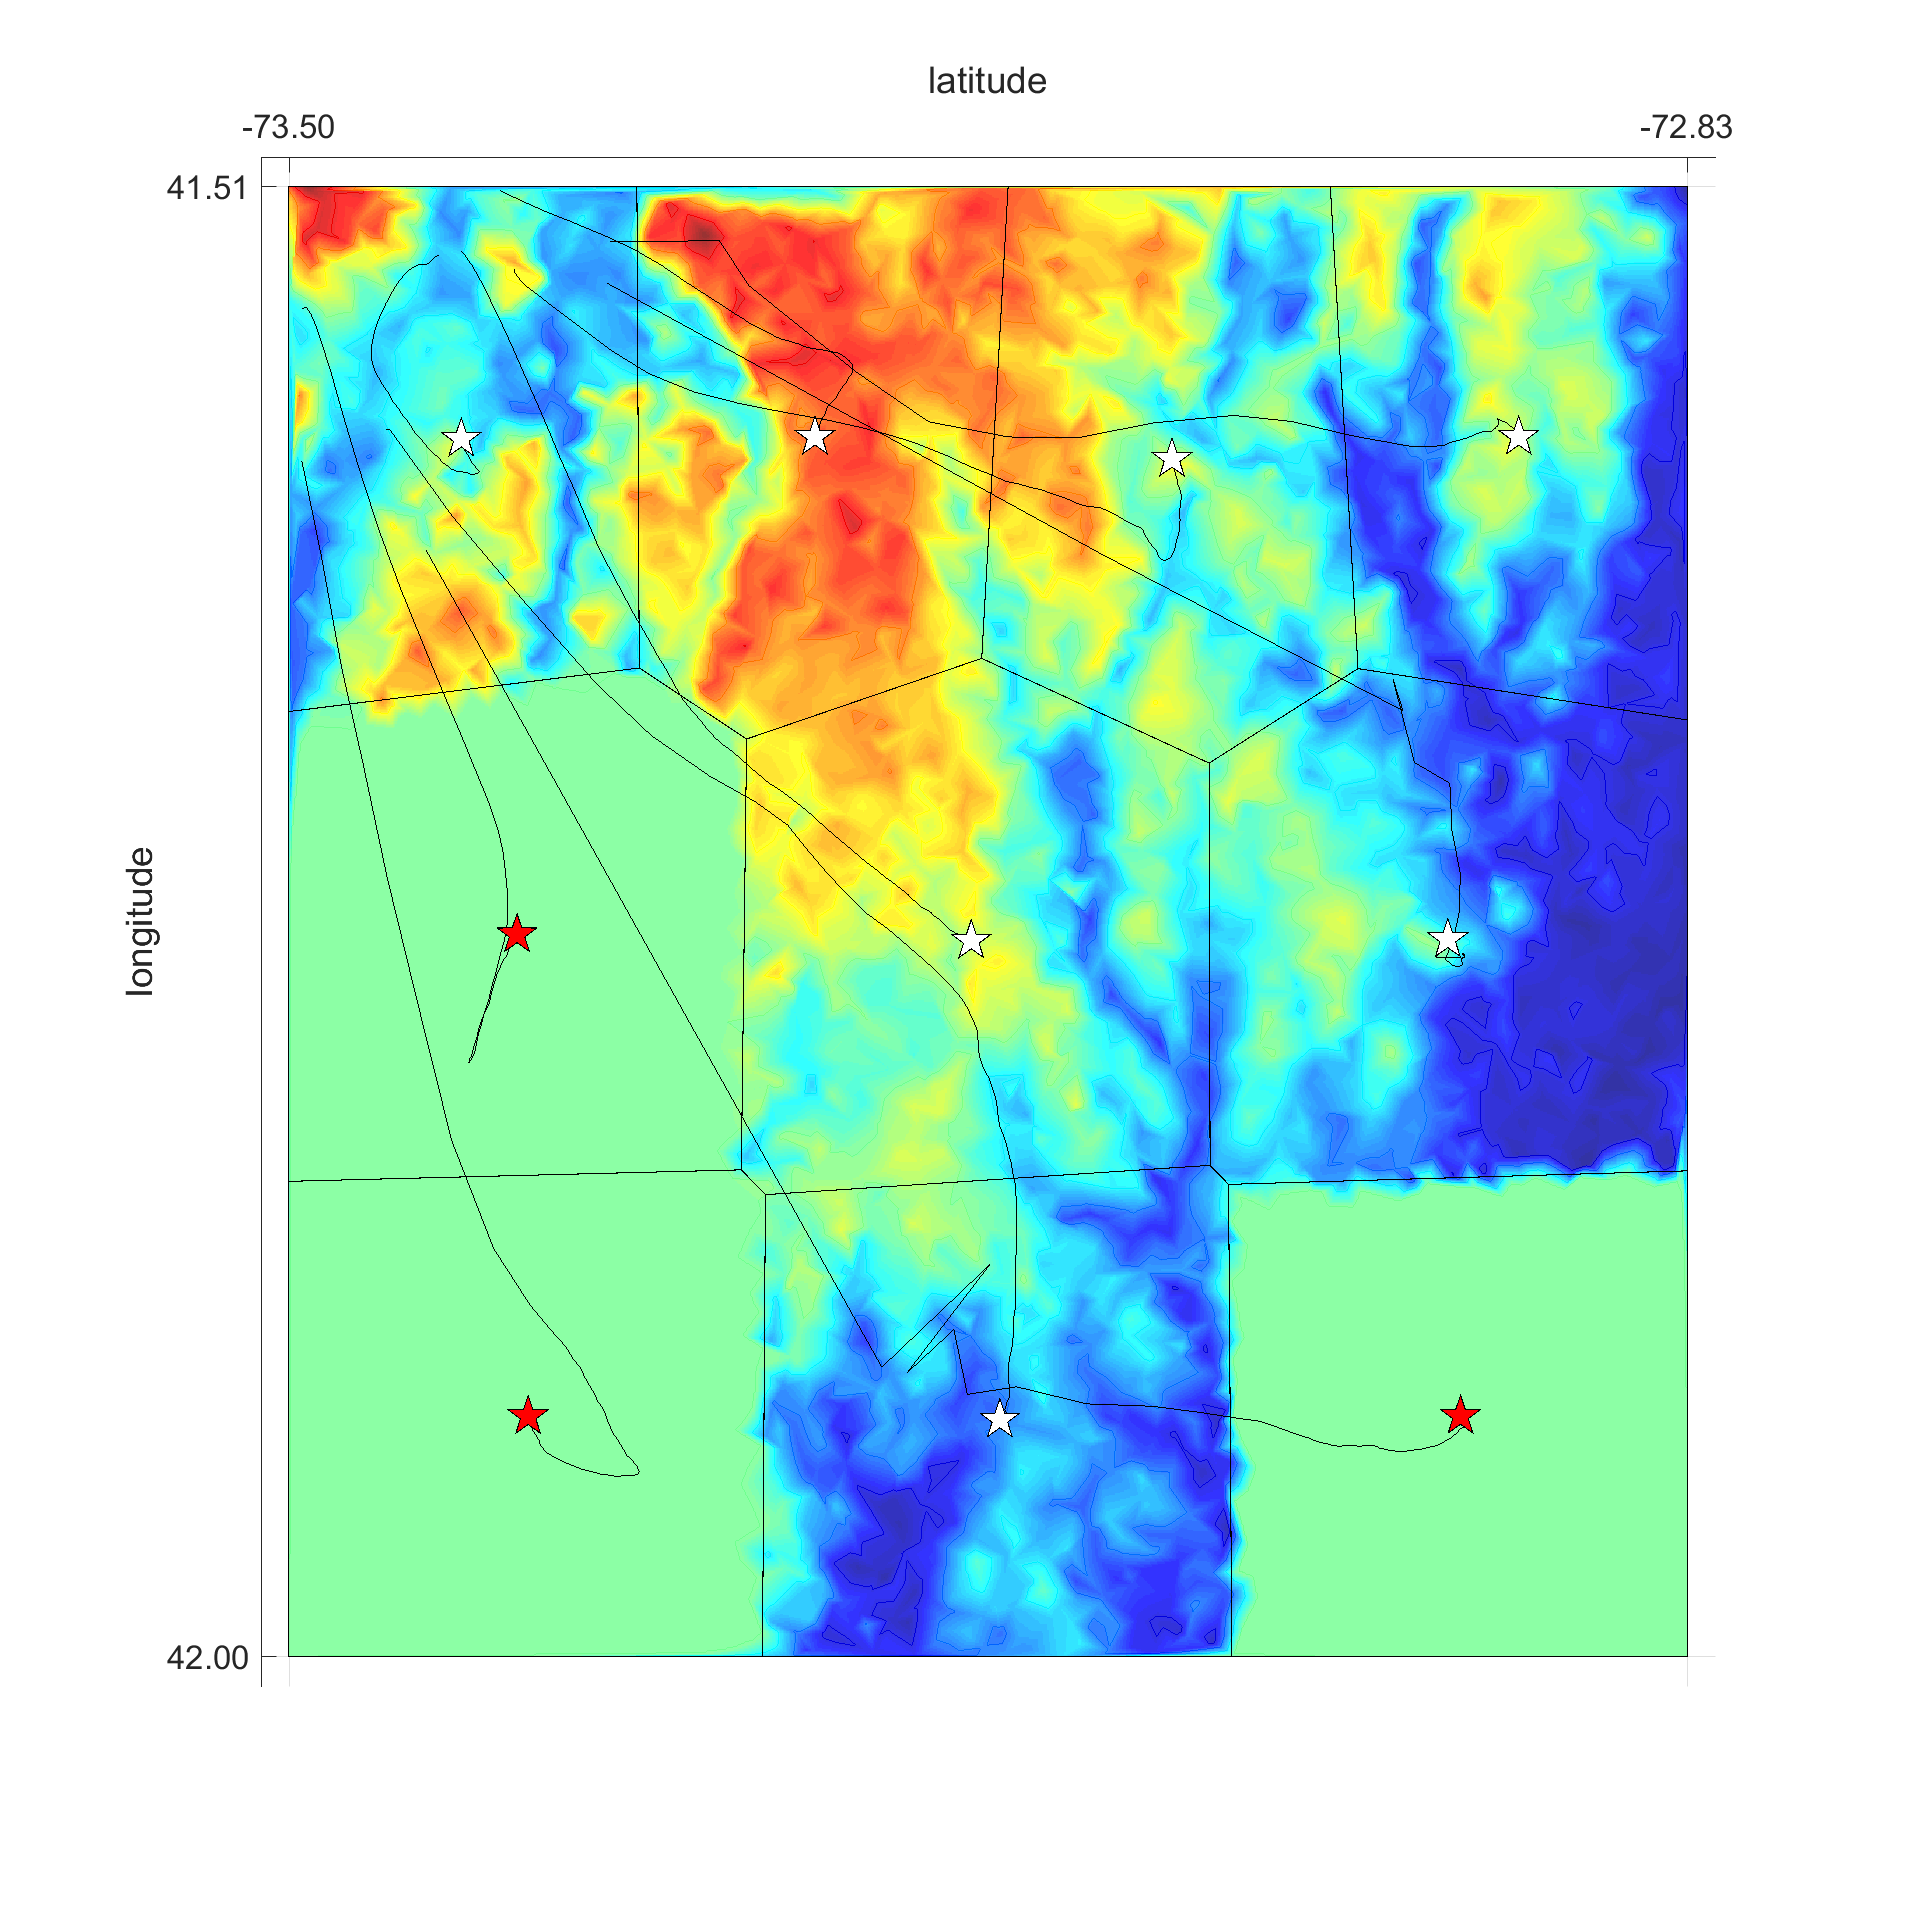
\includegraphics[width=1.57in]{figure/final_config_order1_fault}
	%	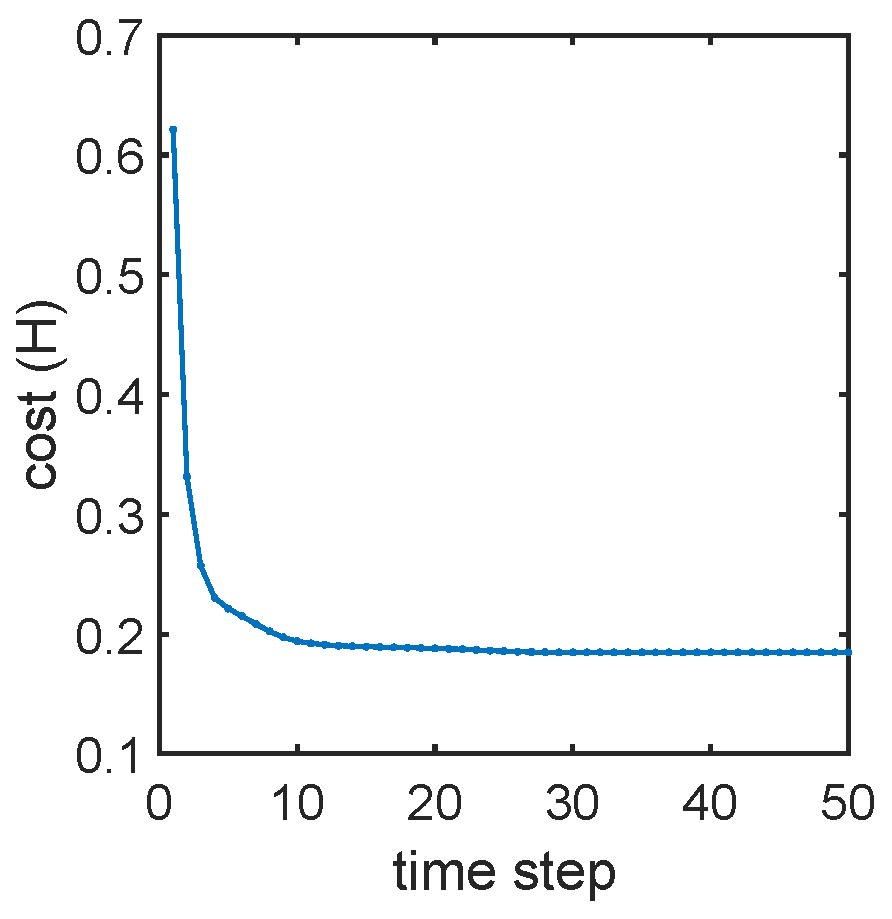
\includegraphics[width=3.4in]{figure/init_10_deploy_cmd2}
	\caption{Simulations with 50 robots where 20 sensors have failed.}
	\label{fig:fig9}
\end{figure}

%\section{An example: Precipitation Mapping using Windshield Wiper Data}
%\label{sec:sec8}
%Existing methods for precipitation measurements (e.g., weather radar, stationary rain guages, etc) usually do not pose high enough temporal resolution for building a precipitation map to be used for time critical hydrological applications, such as, urban flash floods monitoring. In this section, we provide an example based on real-world data which shows that our Bayesian update scheme can be used for online precipitation mapping via utilizing the multi-vehicles' real-time windshield wiper data, which is spatially precise, and has much higher temporal resolution than the data collected from other sources.
%The vehicle wiper dataset---obtained from the University
%of Michigan Transportation Research Institute
%(UMTRI)---contains vehicle locations along with their wiper
%intensity data (four normalized intensity modes: $0,0.33,0.66,1$) which is generated at every 2ms. The windshield wiper data is collected from up to 69 vehicles. 
% We consider a rainfall event occurred at the city of Ann Arbor between 21:47 and 22:26 on August 11th in 2014 (in UTC time). As shown in Fig \ref{fig:fig8}, the rectangular area, $[-83.8,-83.66] \times [42.22,42.34]$ (longitude, latitude in GPS coordinates, respectively) contains the boundary of Ann Arbor, which is drawn by lines. We assume that driver in each vehicle turns on the windshield wiper when detecting rain, and turns it off, otherwise, immediately in both cases. In addition, each driver is assumed to be capable of detecting rain from up to $1$ mile away from the source of rain (i.e., $r_{\textup{eff}} = 1$). We consider a product of two Gaussians---one with covariance matrices $\mathbf{I}$ (unit: mile) for detection, and the other with $0.5\mathbf{I}$ (unit: normalized wiper intensity) for the intensity measurement, respectively---as the windshield wiper sensor model. Since, we did not have control over the vehicles at the time, the map is updated merely using the passively gathered windshield wiper measurements without utilizing our deployment algorithm, namely, Algorithm \ref{alg1}. For our algorithm, the initial expected wind wiper intensity is uniformly set to $0.3$ out of $1$ over the whole region. 
%Fig \ref{fig:fig8} shows two time series of precipitation maps generated by the two different methods where we the wiper data is sampled at every 1 second, and the radar is sampled at every 5 minute.
%The 1st row of Fig. \ref{fig:fig8} shows incremental mapping by our method (non-coordinated strategy, $k=1$). The color intensity shows the relative windshield wiper intensity where brighter area implies relatively more precipitation, and the black area means no precipitation\footnote{We have experimentally validated that there are very strong correlation between windshield wiper intensity and the actual precipitation rate by comparing the windshield wiper data and visual data from the in-vehicle mounted camera.}
%The figures shown in the 2nd row of Fig. \ref{fig:fig8} illustrates the instantaneous precipitation rate measured by the 
%NOAA Next Generation Radar Level III (NEXRAD-III).
%The radar is a Doppler type which is located at Detroit, the nearest NOAA's station to the city of Ann Arbor. 
%%The windshield wiper measurements do not provide the specific  precipitation data as the radar does, nevertheless, the color intensities was used to compare the difference between the two maps.
%
%The rough visual correlation that is shown between the two series of maps shown in Fig \ref{fig:fig8}, especially at the later time (22:26:00) is, unfortunately, not sufficient to validate the real-world performance of our method. 
%There can be numerous reasons for the dissimilarity between the two. In the following, we will discuss a few of them briefly. First, weather radar observations are known to frequently provide unreliable information, e.g., due to blocking or deflection of radar beam, non-precipitation echo (see, e.g., \cite{berg2016creation} to find more details on this topic). In other words, the radar measurements are not consistent enough to be used as the ground truth precipitation data.
%Second, relative to the size of the region of interest, the number of vehicle (only up to 4 vehicles were active during the rainfall event shown in this example) is not large enough to capture the spatial rainfall distribution reasonably well.
%Lastly, our assumption on the effective sensor range for drivers could have been either too restrictive or unrealistic.
%
%
%\begin{figure}
%	\centering
%	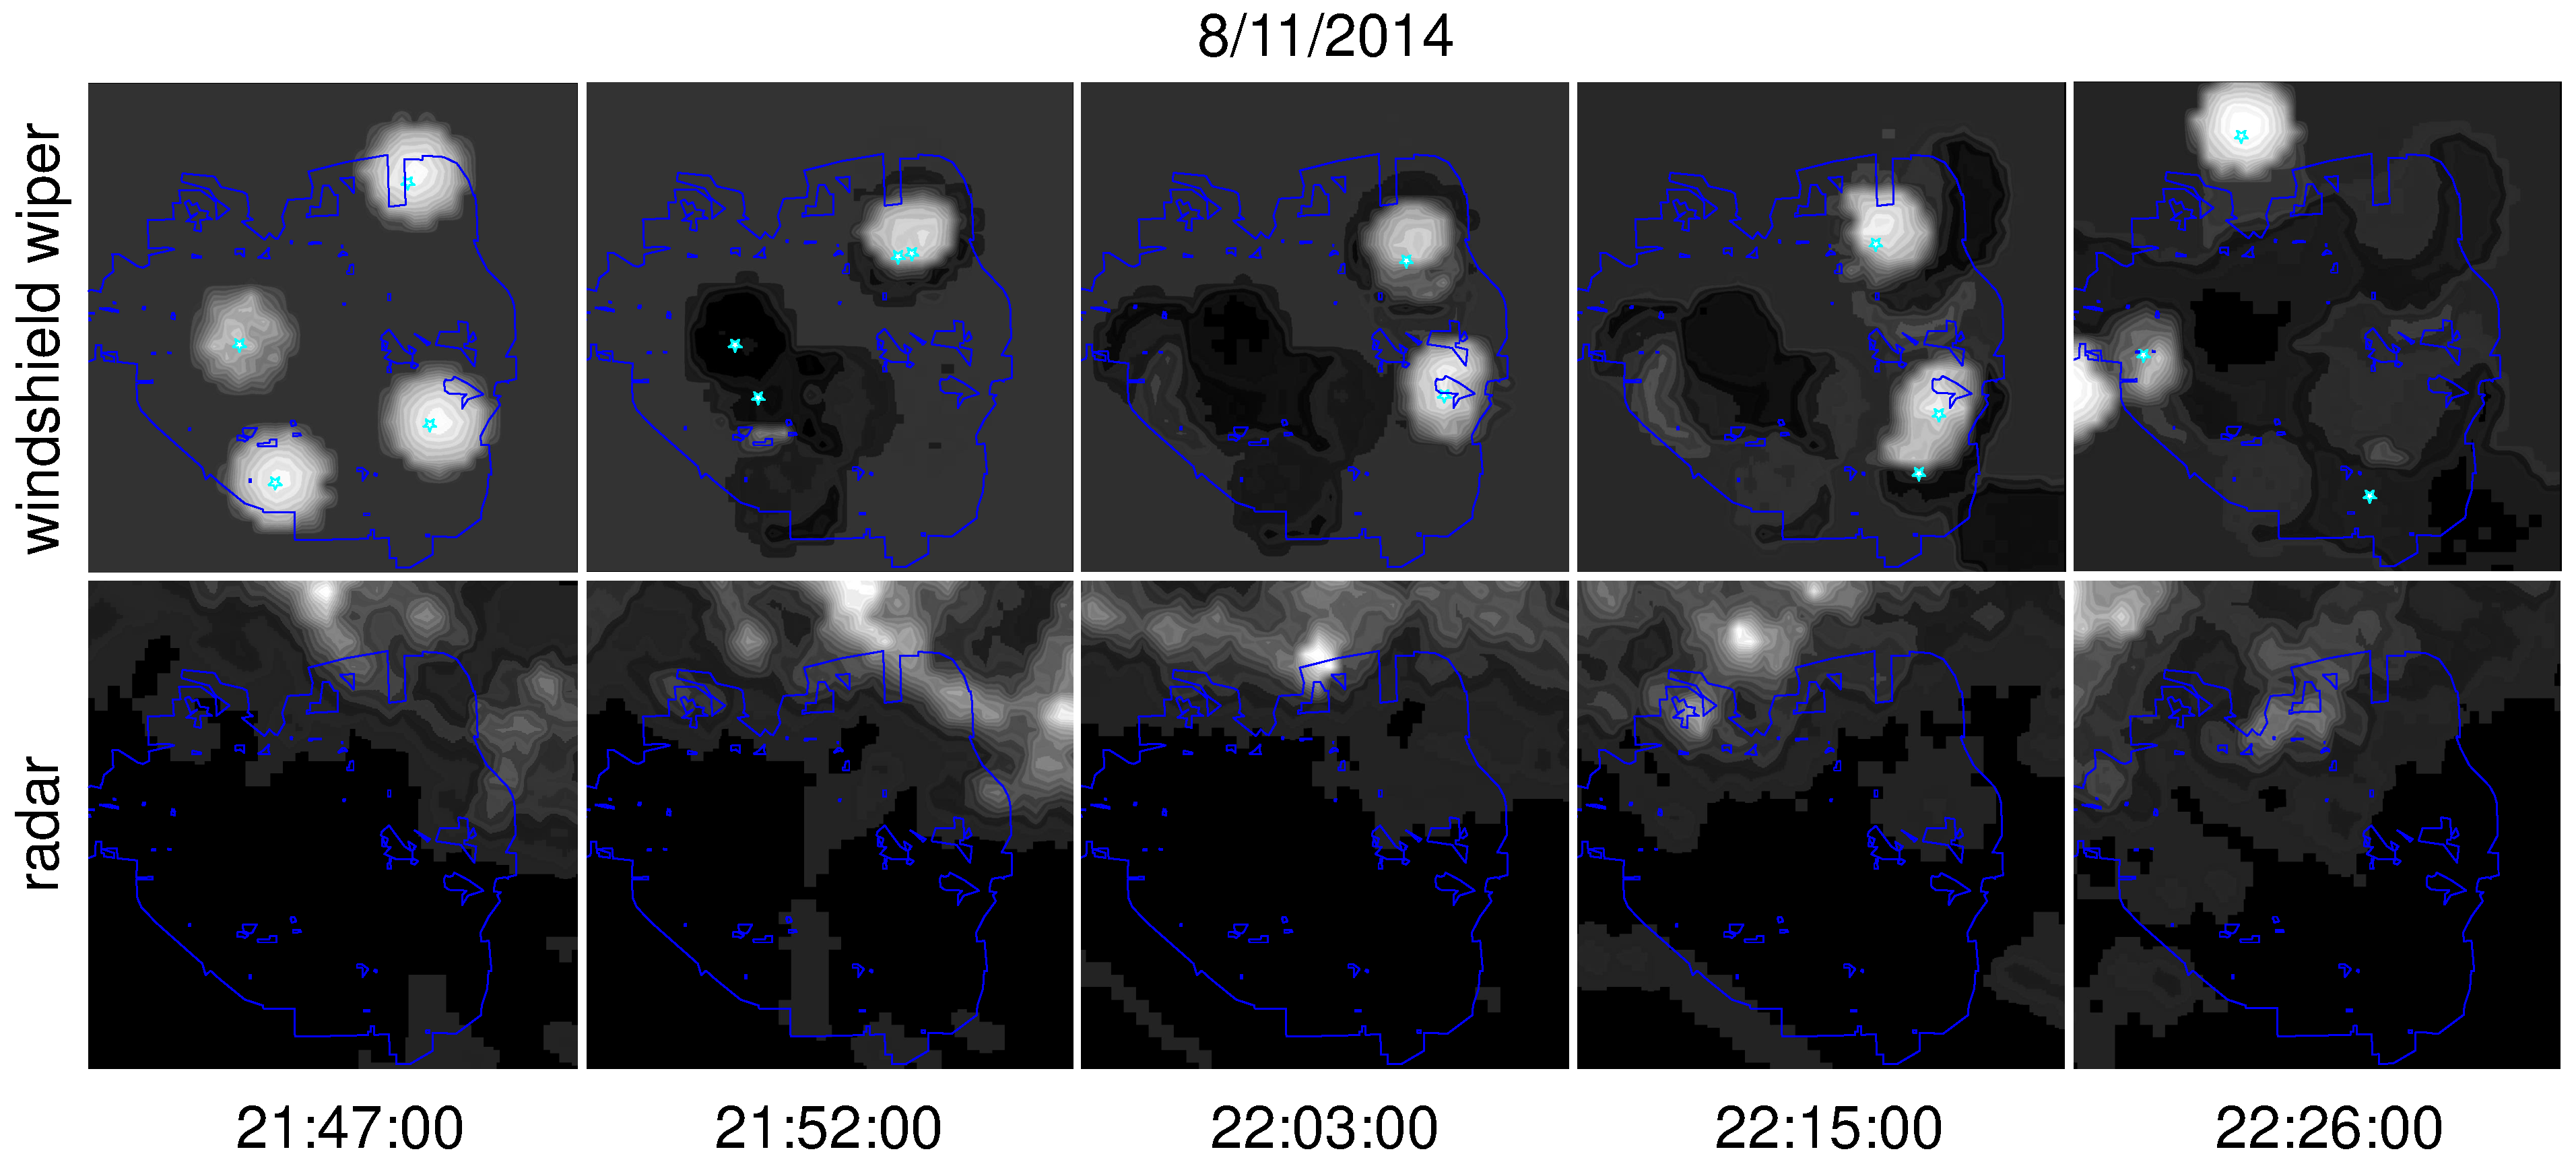
\includegraphics[width=3.5in]{figure/wind_wiper_data3}
%	\caption{A time series of precipitation map build by windshield wiper data collected from up to 4 vehicles using our Bayesian estimator (top row) vs a time series of map built by instantaneous precipitation rate measurements from NEXRAD-III (bottom row). Both maps are generated over the city of Ann Arbor, MI, USA (lines: boundary of the city, stars: vehicles' locations, color intensity: relative precipitation rate where the maximum precipitation rate by the radar is 2in/hr)}
%	\label{fig:fig8}
%\end{figure}


\section{Conclusions and Future Work}
\label{sec:sec9}
This paper presents a general deployment strategy for autonomous fleet to maximize the recovery of environmental map over a bounded space, robots to sensor failures. 
It is expected that our method will fail if there is not enough number of mobile agents having sufficiently long effective sensing ranges compared to the workspace size. 
One of our future works is, therefore, to develop multi-agent patrolling algorithms (see e.g., \cite{portugal2011survey}) to resolve such problems where there may not be enough sensors to cover the whole target space.
Also, as reported in the literature \cite{anguelov2004detecting}, our combined sensor model has been adopted to emulate the real-world laser scanner's behavior, nevertheless, it is one of our future works to conduct extensive real world multi-robot experiments for further validation of our range sensor model.
Lastly, we assumed in this study that the beliefs are shared between robots such that both tasks of information gathering, propagating and approximating belief require a central entity. 
In the future, we will explore how to devise distributed communication protocol to enable distributed belief estimation. 
%\section{type of sensors}

\bibliographystyle{IEEEtran}
\bibliography{reference_park_17}

% that's all folks
\end{document}


